\documentclass[11pt,]{article}
\usepackage[left=1in,top=1in,right=1in,bottom=1in]{geometry}
\newcommand*{\authorfont}{\fontfamily{phv}\selectfont}
\usepackage[]{mathpazo}


  \usepackage[T1]{fontenc}
  \usepackage[utf8]{inputenc}



\usepackage{abstract}
\renewcommand{\abstractname}{}    % clear the title
\renewcommand{\absnamepos}{empty} % originally center

\renewenvironment{abstract}
 {{%
    \setlength{\leftmargin}{0mm}
    \setlength{\rightmargin}{\leftmargin}%
  }%
  \relax}
 {\endlist}

\makeatletter
\def\@maketitle{%
  \newpage
%  \null
%  \vskip 2em%
%  \begin{center}%
  \let \footnote \thanks
    {\fontsize{18}{20}\selectfont\raggedright  \setlength{\parindent}{0pt} \@title \par}%
}
%\fi
\makeatother




\setcounter{secnumdepth}{3}

\usepackage{longtable,booktabs}

\usepackage{graphicx,grffile}
\makeatletter
\def\maxwidth{\ifdim\Gin@nat@width>\linewidth\linewidth\else\Gin@nat@width\fi}
\def\maxheight{\ifdim\Gin@nat@height>\textheight\textheight\else\Gin@nat@height\fi}
\makeatother
% Scale images if necessary, so that they will not overflow the page
% margins by default, and it is still possible to overwrite the defaults
% using explicit options in \includegraphics[width, height, ...]{}
\setkeys{Gin}{width=\maxwidth,height=\maxheight,keepaspectratio}

\title{Estudio de la biodiversidad de Myrtaceae en la Isla de Barrio Colorado,
Panamá. Desde la Ecología Numérica.\\
\emph{Biodiversity study of Myrtaceae on the Island of Barrio Colorado,
Panama. From Numerical Ecology}.  }



\author{\Large Darihana Linares Laureano\vspace{0.05in} \newline\normalsize\emph{Estudiante de Licenciatura en Geografía mención recursos naturales y
ecoturismo, Universidad Autónoma de Santo Domingo (UASD)}  }


\date{}

\usepackage{titlesec}

\titleformat*{\section}{\normalsize\bfseries}
\titleformat*{\subsection}{\normalsize\itshape}
\titleformat*{\subsubsection}{\normalsize\itshape}
\titleformat*{\paragraph}{\normalsize\itshape}
\titleformat*{\subparagraph}{\normalsize\itshape}

\titlespacing{\section}
{0pt}{36pt}{0pt}
\titlespacing{\subsection}
{0pt}{36pt}{0pt}
\titlespacing{\subsubsection}
{0pt}{36pt}{0pt}





\newtheorem{hypothesis}{Hypothesis}
\usepackage{setspace}

\makeatletter
\@ifpackageloaded{hyperref}{}{%
\ifxetex
  \PassOptionsToPackage{hyphens}{url}\usepackage[setpagesize=false, % page size defined by xetex
              unicode=false, % unicode breaks when used with xetex
              xetex]{hyperref}
\else
  \PassOptionsToPackage{hyphens}{url}\usepackage[unicode=true]{hyperref}
\fi
}

\@ifpackageloaded{color}{
    \PassOptionsToPackage{usenames,dvipsnames}{color}
}{%
    \usepackage[usenames,dvipsnames]{color}
}
\makeatother
\hypersetup{breaklinks=true,
            bookmarks=true,
            pdfauthor={Darihana Linares Laureano (Estudiante de Licenciatura en Geografía mención recursos naturales y
ecoturismo, Universidad Autónoma de Santo Domingo (UASD))},
             pdfkeywords = {RStudio, Diversidad, Ecología numérica, BCI, Myrtaceae, coeficientes de
asociación, cluster análisis, ordenamiento, autocorrelación.},  
            pdftitle={Estudio de la biodiversidad de Myrtaceae en la Isla de Barrio Colorado,
Panamá. Desde la Ecología Numérica.\\
\emph{Biodiversity study of Myrtaceae on the Island of Barrio Colorado,
Panama. From Numerical Ecology}.},
            colorlinks=true,
            citecolor=blue,
            urlcolor=blue,
            linkcolor=magenta,
            pdfborder={0 0 0}}
\urlstyle{same}  % don't use monospace font for urls

% set default figure placement to htbp
\makeatletter
\def\fps@figure{htbp}
\makeatother

\usepackage{pdflscape} \newcommand{\blandscape}{\begin{landscape}}
\newcommand{\elandscape}{\end{landscape}} \usepackage{float}
\floatplacement{figure}{H}
\newcommand{\beginsupplement}{ \setcounter{table}{0} \renewcommand{\thetable}{S\arabic{table}} \setcounter{figure}{0} \renewcommand{\thefigure}{S\arabic{figure}} }


% add tightlist ----------
\providecommand{\tightlist}{%
\setlength{\itemsep}{0pt}\setlength{\parskip}{0pt}}

\begin{document}
	
% \pagenumbering{arabic}% resets `page` counter to 1 
%
% \maketitle

{% \usefont{T1}{pnc}{m}{n}
\setlength{\parindent}{0pt}
\thispagestyle{plain}
{\fontsize{18}{20}\selectfont\raggedright 
\maketitle  % title \par  

}

{
   \vskip 13.5pt\relax \normalsize\fontsize{11}{12} 
\textbf{\authorfont Darihana Linares Laureano} \hskip 15pt \emph{\small Estudiante de Licenciatura en Geografía mención recursos naturales y
ecoturismo, Universidad Autónoma de Santo Domingo (UASD)}   

}

}








\begin{abstract}

    \hbox{\vrule height .2pt width 39.14pc}

    \vskip 8.5pt % \small 

\noindent La ecología númerica resulta sumamente importante en el estudio de la
biodiversidad de las plantas, ya que se pueden emplear herramientas
diversas para los estudios multivariacos. El estudio de los conjunto de
datos ecológicos usando algoritmos, permite un aprovechamiento más
detallado y especifico de la familia arbórea, sobre su distribución, el
comportamiento con respecto a variables ambientales, la diversidad de
especies en sitios especificos o su autocorrelación espacial. El estudio
de la biodiversidad de las \emph{Myrtaceae} en las parcelas de medición
permanente en BCI, indican que las especies especies más raras como
\emph{Chamguava schippi} tienden a ser indicadoras de sitios (14 y 19),
influenciadas por variables de suelos como Aluminio Y pH ácido. Se
distinguen patrones de dispersión para variables ambientales com
heterogeneidad ambiental, pico, interfluvio, hombrera, entre otros.


\vskip 8.5pt \noindent \emph{Keywords}: RStudio, Diversidad, Ecología numérica, BCI, Myrtaceae, coeficientes de
asociación, cluster análisis, ordenamiento, autocorrelación. \par

    \hbox{\vrule height .2pt width 39.14pc}



\end{abstract}


\vskip 6.5pt


\noindent  \section{Introducción}\label{introducciuxf3n}

Desde mediados del siglo XVII es posible visualizar el interés del
hombre a estudiar la flora, la fauna y el medio en el que están en
conjunto con las interacciones que se producen entre ellos, pero no es
hasta mediados del siglo XIX cuando se introduce el término Ecología y
su definición, que se empieza a englobar en este tipo de estudios en una
categoría (De la Llata Loyola, 2003). A partir de este punto se
reconocieron distintos campos de estudios y se implementaron nuevos
métodos de análisis, entre los cuales destacan la ecología numérica y
métodos como el análisis multivariático. Según P. Legendre \& Legendre
(2012), la ecología numérica no es más que una de las disciplinas de la
ecología cuantitativa, la cual a la vez es una de las divisiones de la
ecología matemática.

La ecología numérica se concentra en el estudio y análisis de conjuntos
de datos ecológicos, a fin de poder detallar y comprender la
configuración de los conjuntos de datos, combinando diversas
perspectivas numéricas y disciplinas, procedentes de la Geografía, las
matemáticas físicas, taxonomía numérica, parámetros estadísticos y otros
más (P. Legendre \& Legendre, 2012). El análisis de conjuntos de datos
ecológicos, especialmente de la flora, resulta importante tanto para la
ciencia, como para la economía o el sector de salud, por eso se han
establecido distintas parcelas permanentes de medición y monitoreo
forestal donde se colectan datos sobre la diversidad forestal, su
estructura, el crecimiento y su productividad (Pineda, 2014). En el
estudio de las plantas a través de la Ecología Numérica se usan diversas
técnicas que permiten obtener información sobre el rango de asociación,
agrupamiento, ordenamiento, diversidad, autocorrelación, etcétera,
diferentes herramientas para usar las técnicas.

La medición de la asociación es un coeficiente que sirve para medir y
asociar los datos de variables cualitativos y cuantitativos. La medición
de estas variables se puede hacer por dos modos el \emph{Q} y el
\emph{R}, el primero consiste en hacer una comparación de un dúo de
objetos y el segundo consiste en realizar una descripción de un par de
objetos y luego compararlos. Para el modo \emph{Q} se miden la
asociación según la similitud o disimilitud de un par de objetos.
Mientras que para el modo R se mide el grado de dependencia existente
entre las variables, entre los cuales se puede mencionar la covarianza o
el coeficiente de correlación (Borcard, Gillet, Legendre, \& others,
2011).

En cambio, el análisis de agrupamiento o clúster análisis es una técnica
que consiste en separar un conjunto de datos y luego estructurarlos, sin
dejar uno fuera de lugar, como subconjuntos con distintas categorías o
jerarquías de acuerdo a sus características. La finalidad de hacer un
agrupamiento es identificar los pequeños grupos dispersos en un espacio
discreto pero constante, este agrupamiento divide en conjunto de objetos
a estudiar, por lo que es necesario e importante que cada objeto
agrupado en otros subgrupos no se encuentre en otros (Borcard et al.,
2011).

En el caso del análisis de ordenamiento, son técnicas que consisten en
simplificar la magnitud de los datos. Todas estas técnicas muestran las
predisposiciones esenciales de variabilidad de cada dato que se
encuentran en un campo de dimensiones simplificadas, organizando los
ejes con rangos decreciente de varianza explicada en cada uno de los
ejes sucesivo, de forma convencional. Estos tipos de análisis pueden ser
tanto no restringido o simple, como restringido o canónico. En donde
para el primero, las tendencias o predisposiciones del grupo que
interesa no está restringida por otro grupo. Entre sus técnicas
principales de análisis están los de componentes principales
(\emph{PCA}) basado en un vector propio y se utiliza en datos
cuantitativos sin tratamiento preservando la distancia euclídea, los de
correspondencia (\emph{CA}) que se usa en datos frecuentes con
dimensiones uniformes y positivos, y los de coordenadas principales
(\emph{PCoA}) que se concentra en organizar las matrices de
disimilaridad, usualmente, con el modo \emph{Q} en vez de tablas de
sitio por variables (Borcard et al., 2011).

Mientras que, para el segundo análisis de ordenamiento, restringido o
canónico, a diferencia de la simple, es una técnica que relaciona dos o
más conjunto de datos en el proceso de organización u ordenación.
Algunas de sus técnicas principales son análisis de redundancia
(\emph{RDA}) que consiste en la combinación de la regresión y \emph{PCA}
que funciona como una extensión de diversos análisis que muestran la
respuesta multivariante de datos, y el análisis de correspondencia
canónica (\emph{CCA}) que funciona como un aproximado de una regresión
Gaussiana multivariante, además, este se caracteriza por organizar las
especies en todos los ejes canónicos acore a su configuración ecológica
óptima (Borcard et al., 2011).

En cuanto a la diversidad, según Borcard et al. (2011) y Magurran
(1988), esto alude a la variedad y cantidad de especies en un espacio
determinado, esta variedad también se produce a nivel de comunidad. La
diversidad puede La diversidad va desde la diversidad local, hasta
heterogeneidad espacial de esta diversidad. La diversidad de especies
considerada como un número único puede ser medida por la riqueza o la
rarificación de especies usando la notación q o por la presencia o
ausencia de los datos de esta. Según Whittaker (1972), el entendimiento
de la diversidad y los cambios que conllevan, asociados a la
configuración del relieve los componentes \emph{alpha}, \emph{beta} y
\emph{gamma} serian de mucha utilidad. Donde la primera se refiere a la
riqueza de las especies existentes en una comunidad determinada,
considerada homogénea. La segunda, se trata del rango de cambios que se
producen en la estructura de especies que están en diferentes
comunidades en un espacio. Y la última, se refiere a la riqueza de
especies de forma conjuntiva que hay en una comunidad y que integra un
espacio determinado.

La autocorrelación, según Borcard et al. (2011), forma parte de los
análisis espaciales aplicados a datos ecológicos, que se produce por
distintos procesos y que mide puntos cercanos para afirmar si estos
poseen valores similares o distintos, por lo que la correlación puede
ser una correlación positiva o negativa.

La \emph{Myrtaceae} son una familia de plantas de árboles y arbustos
bastante numerosas compuestas caracterizadas por ser leñosas. Esta
familia de plantas pertenece al orden de los \emph{Myrtales}, teniendo a
nivel mundial 129 géneros y aproximadamente 5330 especies; en Panamá 17
géneros y 72 especies; y en Barro Colorado 6 géneros y 15 especies, de
las cuales hay 4 géneros y 7 (ver tabla \ref{tab:genero}) especies en la
parcela de medición permanente (Perez \& R, s.f.; Smithsonian Tropical
Research, 2021). De sus características físicas se destacan sus hojas
simples y opuestas, tienden a ser perennes por lo que resulta poco común
ver individuos caducifolios, sus flores son hermafroditas y comúnmente
son de color blanco con simetría radial, según la especie de esta
familia los frutos tienen forma de bayas o cápsulas secas. De esta
familia el género más conocido es el \emph{Eucalypto Eucalyptus} por sus
propiedades medicinales y su madera dura. Esta familia está distribuida
en todos los continentes, pero predominan en América, África y Oceanía,
en climas templados, tropicales y subtropicales. Muchos consideran que
la importancia de esta familia está en lo económico, como la producción
de frutas para venta de zumos y mermeladas, producción de madera,
producción de papel, de carbón, además de ser usadas en la industria
farmacéutica, se usa en la cosmetología y en la producción de especias
(Almeida, 2019; Britannica, 2016; Lorenzo-Cáceres, s.f.).

El estudio de la biodiversidad de la flora en especial de una especie
vegetal es importante, debido a que permite conocer sus características
propias, ecosistémicas, su distribución, su capacidad productiva, su
potencial de uso y aportes a los humanos como a su ecosistema. Por todo
lo anterior, es importante saber: si los grupos de mi familia,
\emph{Myrtaceae}, se organizan de forma discontinua y acorde a la
composición de las especies; también, si existe algún tipo de patrón que
sea o no sea consistente con alguna variable ambiental o atributo; del
mismo modo, cuántas especies indicadoras hay o si hay alguna con
preferencia por ciertas condiciones ambientales o atributos; de igual
manera y en un espacio bidimensional, si hay una tendencia de ordenación
visible de las especies de Myrtaceae; luego, determinar si las
tendencias de ordenación se asocian con las variables ambientales o
atributos; determinar, de acuerdo a la estimación de riqueza, si mi
familia está bien representada, tomando como buena representación un
85\%; asi mismo, si existe una alguna asociación entre la diversidad
Alpha y las variables ambientales o atributos y cuales son estas;
también, ver si hay algún tipo de contribución local o de alguna especie
a la diversidad Beta; así también, saber si hay alguna especie que
presente algún patrón aglomerado, cuál es y si presenta alguna
asociación con las variables ambientales; y determinar si los modelos de
distribución de especies (\emph{SDM}) predicen adecuadamente las
ocurrencias de las especies.

\section{Área de estudio}\label{uxe1rea-de-estudio}

El área usada para este estudio se encuentra en \emph{BCI} (Isla de
Barrio Colorado), que es una isla perteneciente a Panamá, la cual se
formó cuando las aguas del río Chagres fueron represadas para construir
el Canal de Panamá. Es considerada como una colina con una superficie de
1,500 hectáreas sobresaliente a 137 m en el lago Gatún, y que está
localizada entre los 9\(^\circ\) 09' N y 79\(^\circ\) 51' W. Esta isla
se caracteriza por sus suelos arcillosos con profundidades entre los 50
cm y 1 m, y su clima es común de las tierras bajas tropicales con
temperatura promedio anual de 27\(^\circ\) C, y variación diurna de
9\(^\circ\) C. También tiene unas precipitaciones anuales de 2,600 mm,
con su estación lluviosa (mayo a diciembre), y su estación seca para el
resto de los meses (Pérez et al., 2005; Sugasti, Eng, \& Pinzón, 2018).
Según la clasificación de zonas de vida de Holdridge, BCI se encuentra
ubicada en la zona de vida de bosque húmedo tropical; Claver Farías \&
others (1984), dice que conforme a la clasificación de climática de
Köppen esta tiene un clima tropical húmedo con precipitaciones
abundantes; y de acuerdo con el mapa de la ANAM (2000) su vegetación se
caracteriza por tener bosques semicaducifolio tropical de tierras bajas
(Rodríguez-Castro \& Flores, 2021).

El área de estudio, específicamente, es una parcela permanente forestal
para su medición y monitoreo de 50 hectáreas, establecida en 1980 por
Stephen Hubbell y Robin Foster, en el bosque húmedo tropical de
\emph{BCI}. Esta parcela se caracteriza por su forma rectangular con
1000 m de largo y 400 m de ancho, además, esta se ubica en la parte
central de una meseta en la isla (Hubbell, Foster, \& Condit, 2005;
Pérez et al., 2005). Los datos extraídos de las especies forestales de
la parcela se obtuvieron a través de múltiples censos desde 1982 hasta
2015 (un total de 8 censos), en los cuales se hicieron identificación,
marcado y monitoreo de los tallos leñosos individuales de más de 10 mm
de diámetro a altura del pecho. Durante los 35 años se censaron más de
350,000 árboles individuales (Hubbell et al., 2005). Ver figura
\ref{fig:bci_map}.

\begin{figure}
\centering
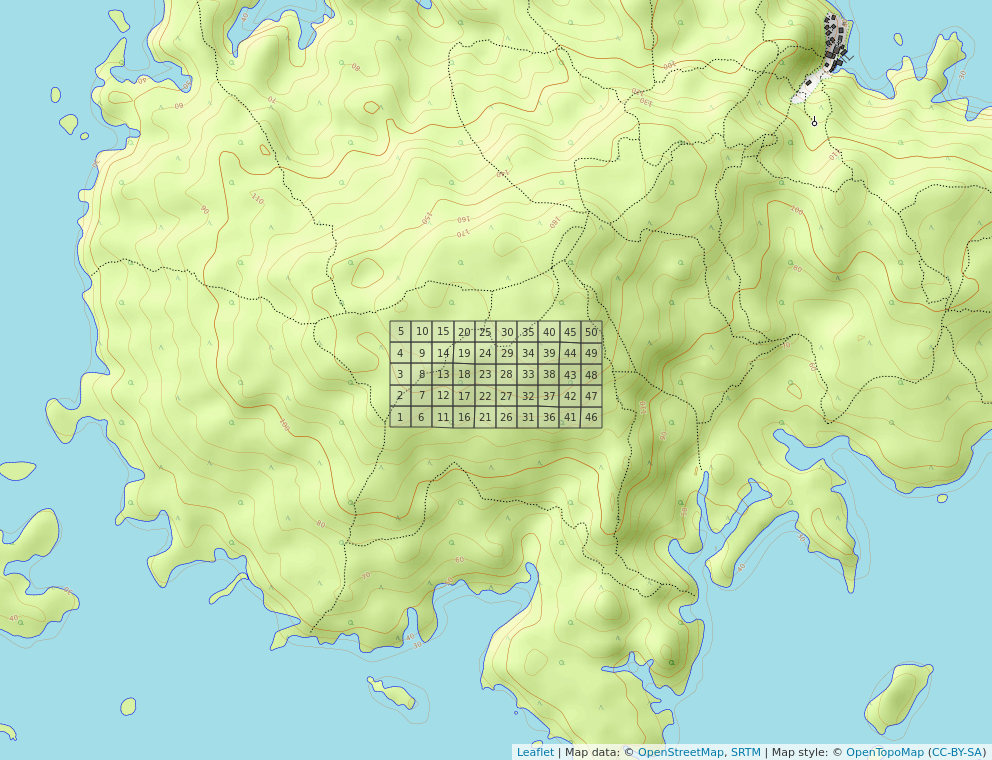
\includegraphics[width=1.00000\textwidth]{mapa_cuadros2.png}
\caption{Mapa de la Isla Barro Colorado y la parcela
permante.\label{fig:bci_map}}
\end{figure}

\section{Metodología y materiales}\label{metodologuxeda-y-materiales}

Para el estudio de la biodiversidad de la familia \emph{Myrtaceae} se
usaron los datos censales de las 50 parcelas forestales de \emph{BCI}
que están presentes en el repositorio \texttt{scripts-de-analisis-BCI}
(Batlle, 2020), de los cuales fueron tratados y procesados con distintos
algoritmos y técnicas de medición, cálculo, análisis e interpretación
por medio del entorno de desarrollo integrado y libre, \emph{RStudio} (R
Core Team, 2020). En cuanto a los gráficos presentes se obtuvieron por
medio \emph{R}, usando paquetes y funciones (ver tabla
\ref{tab:materiales}).

Para iniciar los análisis estadísticos de datos con dimensiones
diversas, Buzai \& Baxendale (2009) y Borcard et al. (2011), recomiendan
realizar un análisis exploratorio de datos (EDA), debido a que es una
herramienta imprescindible para conseguir una primera inmediación,
información genérica de los datos, realizar transformaciones a variables
de ser necesarias, y poder conducir más análisis. Se usaron los paquetes
\texttt{vegan}, \texttt{tidyverse}, \texttt{sf}, \texttt{mapview} y
\texttt{RColorBrewer} para cargar los datos censales, matriz de
comunidad y matriz ambiental, y así poder extraer los datos de la
familia \emph{Myrtaceae}, de las variables ambientales y transformarlos
en tablas, matrices, e incluso generar gráficos de mapas. También, se
usaron las librerías \texttt{psych} y \texttt{ez}, en conjunto con las
anteriores para ver correlaciones de la \emph{Myrtaceae} con distintas
variables ambientales con la función \texttt{cor}, y generar mapas de
variables ambientales por cada cuadro con \texttt{ggplot2}.

La medida de los coeficientes de asociación de la familia
\emph{Myrtaceae} con los modos \emph{Q} y \emph{R} (Borcard et al.,
2011; Salazar, 2000) se realizó mediante funciones pertenecientes a las
librerias \texttt{vegan}, \texttt{adespatial}, \texttt{broom},
\texttt{tidyverse}, \texttt{sf}, \texttt{cluster} y \texttt{gclus}. En
el modo \emph{Q} se mide la abundancia de las especies de
\emph{Myrtaceae} con la función \texttt{dist.ldc} que calcula la
distancia euclídea entre dos sitios y se usa también el método de
transformación Hellinger y así obtener el grado de disimilitud entre
sitios. También, se calculó la distancia de \emph{Jaccard} \emph{Dj}
(Jaccard, 1908; Salazar, 2000) utilizando la función \texttt{vegdist}
que convierte la matriz de comunidad en una de presencia/ausencia para
calcular la matriz de distancia. En cuanto a la asociación de las
variables ambientales, se hizo un nuevo ambiente con la función
\texttt{env} para las variables transformadas con la función
\texttt{scale}. De igual manera, se usó la función \texttt{env\_mix}
para asociar las variables ambientales heterogeneidad ambiental, hábitat
y quebrada, generando una matriz de disimilitud.

Con el modo \emph{R} de medición de asociación, se mensuró el grado de
asociación entre especies haciendo una transformación de la matriz de
comunidad usando la estandarización \emph{Chi} con la función
\texttt{decostand}, luego se calcula la distancia con la función
\texttt{dist} y se representa la matriz en un mapa de calor con la
función \texttt{coldiss}. Se calculó la distancia de \emph{Jaccard}
(Jaccard, 1908; Salazar, 2000) entre especies usando la matriz de
comunidad transpuesta convertida a una de presencia/ausencia con la
función \texttt{vegdist}. En cuanto a la asociación de variables
ambientales numéricas, usando el índice de \emph{rho} de Spearman con
los verbos \texttt{select}, \texttt{mutate} y \texttt{matches} de la
herramienta \texttt{dplyr} y también la función \texttt{cor} para
correlación.

Los análisis de agrupamiento o clúster análisis aplicados a la familia
\emph{Myrtaceae} fueron realizados usando las librerías
\texttt{magrittr}, \texttt{broom}, \texttt{tidyverse}, \texttt{mapview}
y \texttt{indicspecies}. Para el estudio se usó el agrupamiento
jerárquico (\emph{AJ}) con un enfoque aglomerativo por enlace simple,
completo, promedio y el método de \emph{Ward} de varianza mínima
(Borcard et al., 2011). Se agruparon pares de objetos según la mayor
similaridad (vecino más próximo o mínima distancia), partiendo del
agrupamiento por enlace simple, utilizando la matriz de comunidad
transformada por medio del método de normalización con la función
\texttt{decostand} y la distancia euclídea con la función
\texttt{vegdist}. El agrupamiento jerárquico se hizo con la función
\texttt{hclust} para método simple y se generó un dendrograma (gráfico)
con la función \texttt{plot} del resultado de este AJ. Para el
agrupamiento completo usando la menor similaridad (máxima distancia o
vecino más lejano) se empleó la función \texttt{hclust} y la matriz de
distancia de cuerdas o \emph{chord} (Borcard et al., 2011), con tal de
generar un dendrograma con la función \texttt{plot}. En cuanto al
agrupamiento por enlace promedio (UPGMA, WPGMA, UPGMC, WPGMC), se usó el
UPGMA (Romesburg, 2004), para maximizar la correlación entre las
distancias cofenética (coeficiente de correlación de Pearson), para esto
se usó la función \texttt{hclust} y para obtener el gráfico la función
\texttt{plot}. Finalmente, el agrupamiento por Ward (Romero Domínguez,
2021), que define los grupos de una forma donde la suma de cuadrados se
minimice en cada uno de ellos usando las funciones \texttt{hclust} y
\texttt{plot}.

De todos los métodos anteriores de agrupamiento, se han seleccionado
ideal para la familia \emph{Myrtaceae} se usó la función \texttt{map} y
así comparar sus valores. Además, para la elección del número de
clústeres se usó la función \texttt{calcular\_anchuras\_siluetas} en
base a la matriz de comunidad original, la matriz de distancias y objeto
de clúster usando UPGMA y Ward, luego, se hizo un nuevo dendrograma con
la función \texttt{reorder.hclust} y un mapa de calor con la función
\texttt{heatmap}. Finalmente, se hizo una evaluación para ver si el
número de clústeres obtenidos por los métodos anteriores son los ideales
usando el método \emph{bootstrap} (Efron, 1992; Tibshirani \& Efron,
1993), usando el paquete \texttt{pvclust} para generar dendogramas con
trazos en rectángulos y líneas que dividen el gráfico acorde al número
de grupos.

En cuanto al agrupamiento de variables se usaron los grupos obtenidos
por UPGMA para evaluar la homogeneidad por medio de pruebas \emph{t},
basadas en la distribución \emph{t} de \emph{Student} (Hurtado \&
Silvente, 2012) y la suma de rangos de Wilcoxon (Wilcoxon \& Wilcox,
1964), a partir de esto se generaron gráficos de caja y mapas
presentando la ubicación por cuadrado de cada grupo en la parcela
permanente. Y para la homogeneidad de los grupos Ward se usó el método
ANOVA o análisis de varianza (Hurtado \& Silvente, 2012) y
Kruskal/Wallis (Kruskal \& Wallis, 1952).

Cerrando con el clúster análisis, se obtuvieron las especies indicadoras
y las especies con preferencias por hábitats; la primera mediante
\texttt{IndVal} con las funciones \texttt{multipatt} y \texttt{strassoc}
y su significancia o valor p con la función \texttt{p.adjust}; las
especies con preferencias por hábitats se obtuvieron mediante el
coeficiente de correlación biserial puntual (Palmer, Jiménez, \&
Montaño, 2000) con las funciones \texttt{multipatt} y \texttt{strassoc}.

Las técnicas de ordenación aplicas a las \emph{Myrtaceae} usaron las
librerías \texttt{vegan}, \texttt{tidyverse}, \texttt{sf} y
\texttt{mapview}. Para la ordenación simple o no restringida se usaron
las técnicas PCA, CA y PCoA. Con la función \texttt{rda} para escalar
las variables, calcular la matriz de correlación y obtener vectores para
PCA con datos ambientales, la función \texttt{screeplot} para graficar
lo anterior y \texttt{cleanplot.pca} para el escalamiento; también, se
hizo un mapa con puntuaciones de los sitios para tomarlas como
coordenadas con las funciones \texttt{scores} y \texttt{plot}; para
datos de comunidad transformada con \emph{hellinger} se usaron las
funciones \texttt{decostand}, \texttt{rda}, \texttt{screeplot} y
\texttt{scores}, también, se evaluaron los datos de comunidad a datos
ambientales con la función \texttt{envfit}. Para el análisis CA se usó
las funciones \texttt{cca}, \texttt{screeplot} y \texttt{par}. Para el
análisis PCoA se usaron la función \texttt{cmdscale} y una matriz de
distancias, también la función \texttt{ordiplot}.

En la ordenación canónica o restringida se usaron las técnicas RDA y CCA
para presentar las relaciones entre los objetos (entre dos matrices) sin
restricción. En la primera técnica, usando la matriz ambiental, se
utilizaron la función \texttt{decostand}, \texttt{rda} para ajustar las
variables de respuesta por regresión, haciendo prueba estadística para
ver la relación de las variables de la matriz ambiental según el valor
de \emph{p}, también se calculó R2 insesgado con la función
\texttt{RsquareAdj}, además de explorar la multicolinealidad entre
variables. En cuanto a CCA, se usaron las mismas funciones, se
excluyeron especies con abundancias mínimas al 100 por individuo.

En cuanto a la diversidad de la \emph{Myrtaceae}, alpha y beta, para su
cálculo se usaron las librerías \texttt{vegan}, \texttt{adespatial},
\texttt{plyr}, \texttt{RColorBrewer}, \texttt{tidyverse}, \texttt{sf},
\texttt{SpadeR}, \texttt{iNEXT}, \texttt{vegetarian} y \texttt{mapview}.
Para calcular la diversidad especies, alpha, como un número único, se
usó la función \texttt{alpha\_div} y así obtener los índices alpha;
tambien se usó la función \texttt{pairs} para hacer una matriz de
correlación de Pearson con todos los índices, luego con la función
\texttt{bind\_cols} se unen en una matriz estos índices con variables
ambientales. Para calcular el rango de abundancia de especies se usó la
función \texttt{radfit}. Para la rarefacción por sitios se usó la
función \texttt{specnumber}. Para el cálculo de abundancia por sitio se
usó \texttt{rowSums}; se generó con una curva de rarefacción con los
datos obtenidos anteriormente. De la misma manera, se calculó la riqueza
de especies mediante estimaciones y comparaciones y evaluar la
completitud de muestra; para esto se usaron los enfoques asintóticos y
no asintóticos (el primero para estimar riquezas de especies y el
segundo para rarefacción y extrapolar), se calculó y se extrapoló la
riqueza de especies con la función \texttt{specpool}; con la función
\texttt{colSums} se hizo una matriz de comunidad combinando, con medias
númericas, todos los sitios en uno, para estimar, con esta matriz, la
riqueza con el índice \emph{chao} (Chao \& Chiu, 2016), la rarefacción y
extrapolación de especies.

También se aplicaron los enfoques asintóticos y no asintóticos para
generar una matriz de comunidad agrupada según Ward usando los verbos
\texttt{mutate} y \texttt{select}de \texttt{dplyr}; se estimó la riqueza
y los porcentajes bajos y altos con la función
\texttt{estimación\_riqueza\_chao}, también se obtuvo los porcentajes de
rarefacción y se extrapoló. Y para calcular la diversidad beta con único
número se usó la función \texttt{calcular\_beta\_multiplicativa};
también se determinó la contribución de especies y la contribución local
a la diversidad beta con la función
\texttt{determinar\_contrib\_local\_y\_especie} con el método
\texttt{hellinger} y un indicador alpha de 0.05.

Finalmente, se realizó la autocorrelación o análisis espacial ecológico
usando las herramientas de las librerias \texttt{ape}, \texttt{spdep},
\texttt{ade4}, \texttt{adegraphics}, \texttt{adespatial},
\texttt{vegan}, \texttt{tidyverse}, \texttt{sf}, \texttt{gridEstra},
\texttt{grid}, y \texttt{gtable}. Se generó una matriz Hellinger con la
función \texttt{decostand} y se transformó la matriz ambiental con el
objeto \texttt{sp} para generar vecindad, del mismo modo se usó la
función \texttt{nb2listw} para crear una lista de vecinos con pesos
espaciales. También, se hizo una autocorrelación espacial por medio de
correlograma de una sola variable ambiental con la función
\texttt{sp.correlogram}; del mismo modo, se hizo una con múltiples
variables con la matriz de Hellinger para conocer la abundancia de
especies con la función \texttt{calcular\_autocorrelacion} con el método
de Moran's I.

Además, se hizo una versión reversa de la matriz Hellinger con
\texttt{rev} y luego se generaron gráficos con la función \texttt{par}.
De igual manera, se hizo la autocorrelación para las variables
ambientales con la función \texttt{calcular\_autocorrelacion} y el
método de Moran's I. Se hizo, también, una autocorrelación espacial por
medio de la prueba de Mantel (Borcard \& Legendre, 2012) o matrices de
distancias a datos de comunidad con las funciones \texttt{resid},
\texttt{dist} y \texttt{mantel.correlog}. Se realizó una autocorrelación
espacial mediante pruebas de permutación para el I de Moran aplicado a
abundancia de especies transformadas sin tendencia con \texttt{sapply}
usando la función \texttt{mi\_fam\_sin\_tendencia}; aplicado a variables
ambientales, se usó \texttt{sapply} con las funciones \texttt{var},
\texttt{gtable\_filter} y \texttt{grid.arrange} para filtrar celdas por
nombre de las variables ambientales; se usó el mismo procedimiento
aplicado a abundancias de especies transformadas y aplicado a
abundancias de especies transformadas sin tendencias.

\section{Resultados}\label{resultados}

\subsection{Análisis Exploratorio de Datos
(EDA)}\label{anuxe1lisis-exploratorio-de-datos-eda}

La aplicación de los EDA en el estudio produjo informaciones generales
sobre la familia \emph{Myrtaceae}, sus especies, su abundancia, las
variables ambientales, y datos generales de correlación con las
variables ambientales. La parcela de muestreo permanente (de ahora en
adelante \emph{pmp}) de 50 hectáreas en BCI tiene 5579 individuos
(abundancia) pertenecientes a la familia \emph{Myrtaceae} y una riqueza
de 7 especies. Las especies que más destacan por su abundancia son las
\emph{Eugenia galalonensis} (1975 individuos) y \emph{Eugenia
oerstediana} (1838 individuos), en cambio, las especies con menor número
de individuos en la parcela son \emph{Myrcia gatunensis} (56 individuos)
y \emph{Psidium friedrichsthalianum} (50 individuos), ver tabla
\ref{tab:specabu} y figuras \ref{fig:abumifam} y \ref{fig:riqmifam}.

\begin{longtable}[]{@{}cc@{}}
\caption{\label{tab:specabu} Abundancia por especies de la familia
\emph{Myrtaceae}}\tabularnewline
\toprule
Especies & Número\tabularnewline
\midrule
\endfirsthead
\toprule
Especies & Número\tabularnewline
\midrule
\endhead
Eugenia galalonensis & 1975\tabularnewline
Eugenia oerstediana & 1838\tabularnewline
Eugenia coloradoensis & 609\tabularnewline
Chamguava schippii & 541\tabularnewline
Eugenia nesiotica & 502\tabularnewline
Psidium friedrichsthalianum & 58\tabularnewline
Myrcia gatunensis & 56\tabularnewline
\bottomrule
\end{longtable}

De acuerdo con los resúmenes estadístico el 50\% de la abundancia de
especies, según la mediana, es mayor de 541 individuos (\emph{Chamguava
schippii}) y la abundancia de especie promedio en \emph{pmp} es de 797
individuos. En cuanto a la riqueza de la familia \emph{Myrtaceae},
indica que el 50\% de la riqueza, según la mediana, es de 6 especies y
una riqueza promedio de 5.5, también hay que agregar que la riqueza
mínima es de 4 especies en \emph{pmp}. De igual manera, hay que
mencionar que la riqueza y la abundancia varía por cuadro de 1h en
\emph{pmp}, arroja que los sitios con mayor riqueza son los cuadros 13,
14, 17, 22 y 40 (7), en cambio los de menor riqueza son los cuadros 2,
5, 11, 36, 46 y 47 (4); y los sitios con mayor abundancia fueron los
cuadros 19, 20, 15, 40 y 38, y los de menor abundancia fueron los
cuadros 1, 36, 30, 2 y 9; donde coinciden el sitio 40 con mayor riqueza
y abundancia por cuadro, y los sitios 2 y 36 con menor riqueza y
abundancia, lo que indica que existe una distribución aleatoria y
desigual de las riquezas y abundancias en los sitios de \emph{pmp} (ver
figura \ref{fig:abuxcua}). De las especies de \emph{Myrtaceae} que
presentan una correlación simple (de Pearson) positiva significativa, en
comparación a las demás, están \emph{Chamguava schippii} y \emph{Eugenia
galalonensis} con un índice de correlación de 0.30, también
\emph{Chamguava schippii} con \emph{Eugenia nesiotica} con un índice de
correlación de 0.29, por lo que estas especies tiene una relación con la
otra (ver figura \ref{fig:corresp}).

En cuanto a las variables ambientales que se destacan en \emph{pmp}
están: la geológica, que de acuerdo con el Mapa geológico del canal de
Panamá y sus alrededores (R. Stewart, Stewart, \& Woodring, 1980) y los
resultados de EDA la \emph{pmp} se caracteriza, por sus rocas basalto,
tipo intrusiva y extrusiva, del Mioceno medio y superior (Tb). También
se caracteriza por tener hábitats de bosque viejo en relieve bajo en su
mayoría al oeste de la parcela, en algunas partes del centro y al este
de \emph{pmp}; por sus hábitat de bosque viejo en relieve alto al centro
y este de \emph{pmp}; se agregan los bosques jóvenes de los sitios 30 y
35; y los bosques de pendiente baja concentradas al este y con algunos
sitios aleatorios en \emph{pmp}; al final, está el bosque de pantano en
el centro de \emph{pmp} (ver figura \ref{fig:ambvar}).

Por último, se destacan las variables de terreno como elevación media
que predomina la mitad hacía el norte de la parcela en un 50\% en
adelante. También se destaca la forma vertiente del terreno donde en una
escala de o a 1, esta predomina en casi toda la parcela sobre el 50\%.
En cuanto a minerales, el aluminio se manifiesta al oeste de las
parcelas, superior al 50\% y en uno que otro lugar entre la parte este
de la parcela. El hierro se manifiesta en un porcentaje superior al 75\%
al este de la parcela. Finalmente, el pH se manifiesta desde la mitad de
los sitios de la parcela hacia el este como menos acidos y el resto como
ácido (ver figura \ref{fig:varnum}).

\subsection{Asociación de especies y variables
ambientales}\label{asociaciuxf3n-de-especies-y-variables-ambientales}

La asociación presente entre sitios de la parcela, obtenida al calcular
la distancia euclídea usando la matriz de comunidad transformada con el
método de \emph{Hellinger}, señala varios grupos de sitios
extremadamente semejantes, según la matriz de disimilitud ordenada hay
un grupo limitado por los cuadros 20-25; un segundo grupo, cuadros
12-32; un tercer grupo, los cuadros 32-42; un cuarto grupo, los cuadros
34-46; un quinto grupo, los cuadros 43-49; y un último grupo, el sexto,
limitado por los cuadros 16-29; estos lugares comparte una similitud
superior de 70\% (ver figura \ref{fig:matrizdisimord}).

La distancia de \emph{Jaccard} y la distancia de \emph{Bray-Curtis}
presentan un comportamiento distinto en cuanto a los grupos que se
forman por la similaridad, al de distancia euclídea con el método
\emph{Hellinger}. Con el método de \emph{Jaccard} se produjeron 7 grupos
que comparten similitudes mayores al 70\%: el primero limitado por los
cuadros 47-46, el segundo por los cuadros 43-39, el tercero por los
cuadros 24-30, el cuarto grupo por los cuadros 32-22, el quinto por los
cuadros 22-26, el sexto por 48-49, el séptimo y último 45-50. También,
la distancia de \emph{Jaccard} señala la existencia de sitios con
exclusividad considerable, como los sitios 1 y 2 con una exclusividad de
especies del 20\% por lo que tienen similaridad visible de especies del
80\% (ver figura \ref{fig:matrizjacc}). Según la fórmula de similaridad
de \emph{Jaccard} ambos sitios comparten 4 especies, pero el sitio 2 no
tiene especies exclusivas, en cambio, el sitio 1 tiene una especie
exclusiva; según el porcentaje de especies compartida o similaridad, se
confirma que comparten el 80\% de sus especies (ver figura
\ref{fig:riqmifam}).

En cuanto a las variables ambientales, los resultados del análisis de
correlación para las variables de suelo o edáficas indican que hay
similaridades importantes para los sitios limitados por los cuadros
12-16 de la matriz de disimilaridad ordenada (ver figura
\ref{fig:suelodis}), creando lo que es un gran cluster de variables
edáficas muy similares. Mientras que, las variables mixtas
(\texttt{heterogeneidad\ ambiental}, \texttt{habitat} y
\texttt{quebrada}) se aprecia en la matriz de disimilaridad ordenada
(ver figura \ref{fig:mixtadis}) un gigantesco grupo de sitios que
comparten similitudes, estos sitios están limitados por los cuadros
25-27; en este conjunto se puede apreciar la similitud, en específico,
de el cuadro 2 y el 7 con un hábitat de bosque viejo y relieve bajo, en
ambos cuadros hay quebrada y además, poseen unos valores moderados de
heterogeneidad ambiental; si se observan los mapas de riqueza y
abundancia de la familia \emph{Myrtaceae} (ver figuras
\ref{fig:riqmifam} y \ref{fig:abuxcua}), el sitio 2 presenta la riqueza
más baja y una abundancia baja a diferencia del sitio 7 que tiene una
riqueza alta y una abundancia media, por lo que no se considera que
tengan relación con la riqueza y la abundancia de la especie, pero si
tienen una similaridad.

En el caso de los grados de asociación entre las especies, en función de
abundancia, según señala el mapa de calor ordenado (ver figura
\ref{fig:asoespec}) obtenido con el método de transfromación \emph{Chi},
existe un patrón de dependencia alto entre las especies que se
relacionan en la diagonal desde \emph{Eugenia oerstediana} hasta
\emph{Eugenia coloradoensis} (cuadros de color rosa intenso centrales),
y una dependencia moderada entre la especie \emph{Psidium
friedrichsthalianum} y el resto, a excepción de las especies
\emph{Myrcia gatunensis} y \emph{Chamguava schippii} que no presentan
ningún patrón de dependencia con ninguna de las especies de la familia
\emph{Myrtaceae} presente en la parcela de BCI (cuadros de color azul).
Conforme al mapa de calor obtenido por la distancia de \emph{Jaccard},
se confirma la existencia del patrón de dependencia alto entre las
especies relacionadas en la diagonal desde \emph{Eugenia oerstediana}
hasta \emph{Eugenia neosiotica}, dejando a las especies \emph{Psidium
friedrichsthalianum}, \emph{Myrcia gatunensis} y \emph{Chamguava
schippi} como especies sin dependencia alguna según su abundancia (ver
figura \ref{fig:dependenciajacc}).

Para las variables edáficas, los índices de correlación obtenidos por el
método Pearson, indican que existe una relación significativa positiva
de 0.32 entre la abundancia de \emph{Myrtaceae} y el aluminio; del mismo
modo, señala que existen relaciones dependientes positiva entre la
riqueza de \emph{Myrtaceae} y el fósforo (0.36), y el aluminio (0.36),
por lo que el resto de variables edáficas no tienen una asociación
significativa positiva con la distribución de las especies y su
abundancia (ver figura \ref{fig:chivardep}). Lo mismo sucede, usar el
método de \emph{Spearman}, confirmando que existe una relación positiva
significativa entre aluminio y la abundancia de \emph{Myrtaceae},
también, que existe una relación positiva la riqueza de \emph{Myrtaceae}
con el aluminio y con el fósforo; hay que destacar que se obtuvo un
índice correlación negativo significativo entre la riqueza de la familia
y el calcio, por lo que esta variable edáfica y la riqueza de la familia
no tienen ninguna asociación (ver figura \ref{fig:mspearman}).

La correlación de \emph{Pearson} presenta 6 asociaciones significativas
entre las variables geomorfológicas y la abundancia de la familia, una
relación positiva con la geomorfología de \texttt{llanura} (0.51) y con
\texttt{elevación\ media} (0.29), indicando que tienen existe una
dependencia significativa. También se obtuvieron asociaciones negativas
significativas entre la abundancia de la familia y las variables
\texttt{pendiente\ media}, \texttt{vaguada}, \texttt{vertiente} y
\texttt{heterogeneidad\ ambiental} (ver figura \ref{fig:pearson_geom}).
En cambio, la correlación de \emph{Spearman} señala 3 asociaciones
significativas con la abundancia de \emph{Myrtaceae}, de las cuales
coinciden las negativas con las variables de \texttt{vaguada} y
\texttt{heterogeneidad\ ambiental} y una positiva con
\texttt{elevación\ media} (ver figura \ref{fig:spearm_geom}). En el caso
de la riqueza, no existe ninguna correlación significativa con las
variables geomorfológicas en ambos métodos usados, por lo que la riqueza
de la familia no tiene una dependencia considerable con la
geomorfología.

\subsection{Cluster análisis
(Agrupamiento)}\label{cluster-anuxe1lisis-agrupamiento}

El agrupamiento jerárquico de los 50 sitios o cuadros de 1 Ha en BCI,
usando criterios de enlaces aglomerativos simple, completo y por
promedio (UPGMA) y calculados a partir de matriz de distancia de cuerdas
, presentan las mismas tendencias aglomerativas que indican la
existencia de dos grupos de sitios, uno compuesto por dos sitios que se
distinguen del resto (14 y 19 ) como únicos y uno mas grande; en cuanto
al método por Ward, existen dos grupos con más sitios a diferencia del
resto de métodos, aunque los sitios 14 y 19 siguen apareciendo como
grupos únicos, pero están dentro de otro grupo más grande. El enlace
completo presenta, exceptuando el grupo de los sitios 14 y 19, dos
grupos definidos entre los sitios 8-20 y 41-44; con el enlace UPGMA se
aprecia que el sitio 50 es único, lo cual se cumple en los otros enlaces
aglomerativos (ver figura \ref{fig:enlaces}).

En cuanto al número optimo o idóneo de grupos, calculado con el
\texttt{ancho\ de\ silueta}, para el método UPGMA es 2
(\ref{fig:gruposU}); uno pequeño representado por 19 y 14, y uno grande
con el resto, pero que si al observarse se puede ver que este se divide
e dos grupos, entre los sitios 1 y 20 y el otro entre 15 y 49, además se
identifica, como se mencionó anteriormente, la existencia de un lugar
único, el sitio 50 (ver figura \ref{fig:upgmaden}), por lo que el primer
grupo tiene 48 sitios y el segundo solo 2. Y según el criterio de Ward,
el número optimo de grupos es de 3 (\ref{fig:gruposW}), dos grupos
grandes y uno pequeño; el primer grupo esta entre los sitios 20 y 50, el
segundo entre 1 y 18, y el tercer grupo conformado por los sitios 14 y
19 (como en UPGMA), por lo que el primer grupo tiene 20 sitios, el
segundo tiene 28 y el tercer grupo solo 2 sitios (ver figura
\ref{fig:wardden}).

Al evaluar la homogeneidad de promedios de las variables para los grupos
de UPGMA con la prueba \emph{t} de \emph{Student} (medias) indican que
la media de las variables geomorfológicas
\texttt{espolón/gajo,\ vaguada,\ valle,\ interfluvio,\ orientación\ media}
y \texttt{elevación\ media}, y las de suelo
\texttt{zinc,\ boro,\ nitrógeno} y \texttt{calcio}, de ambos grupos
presentan un valor p significativamente diferentes. En el caso de la
suma de rangos de \emph{Wilcoxon} (medianas), no existe ningún valor p
significativo para las variables ambientales (ver figura
\ref{fig:upgma_caja}). Tomando de ejemplo la variable Zinc podemos
observar como sus valores son muy bajos para el grupo dos de UPGMA y
para los sitios del grupo uno se observa que al este del centro los
valores de zinc aumentan de manera significativa, muy distinto a los
sitios del oeste de la parcela (ver figuras \ref{fig:gruposU} y
\ref{fig:zinc}).

Acorde a la evaluación de homogeneidad de variables para los 3 grupos de
Ward, usando la prueba ANOVA (medias), la media de las variables
ambientales
(\texttt{pH,\ zinc,\ boro,\ nitrógeno,\ pendiente\ media,\ espolón/gajo,\ elevación\ media,\ calcio,\ orientación\ media})
de los tres grupos es significativa por lo que son muy diferentes.
Mientras que, para la prueba de Kruskal-Wallis (medianas), solo hay una
variable ambiental con \emph{valor p} significativo y que vuelve a los
tres grupos distintos, la variable \texttt{pH} (ver figura
\ref{fig:ward_caja}). Al observar los mapas de pH (con valor p
significativo) se puede identificar que para los sitios del grupo uno
son altos, para los sitios del grupo dos los valores de pH son de bajos
a moderados y para los sitios del grupo 3 son altos (ver figuras
\ref{fig:gruposW} y \ref{fig:ph}).

En cuanto a las especies indicadoras de cada grupo de los métodos UPGMA
y Ward se calcularon con el indice IndVal. Para los grupos de UPGMA
denota, acorde a su valor de significancia, que solo el grupo dos tiene
una especie indicadora, \emph{Chamguava schippii}, la cual representa a
este grupo al 97.2\%; y se puede confirmar al observar el
\texttt{mapa\ de\ abundancia\ por\ especies\ por\ cuadros}
\ref{fig:abuxcua}, mostrando que efectivamente la abundancia de esta
especie en los sitios del grupo 2 supera por muchísimo a la de otras
especies; hay que agregar que este grupo presenta asociaciones con
algunas variables ambientales que corresponden con su característica
única. Al observar los intervalos de confianza de todas las especies por
grupos, se denota que para el grupo uno no se obtuvieron especies
indicadoras con IndVal,indicando que las especies presentes en este
sitio no tienen una preferencia por el grupo, pero con los intervalos de
confianza, obtenidos con \texttt{strassoc}, se puede concluir que la
especie indicadora para este grupo pueden ser \emph{Eugenia
galalonensis} y \emph{Eugenia oesterdiana} con un valor de confianza de
64\% y 71\%, respectivamente.

Así mismo, el índice IndVal muestra para los grupos de Ward, que solo el
grupo tres tiene una especie indicadora, siendo la misma del grupo dos
de UPGMA, \emph{Chamguava schippii} con un valor de confianza del
97.2\%. Pero, de acuerdo con los intervalos de confianza, obtenidos con
\texttt{strassoc}, podemos concluir que para el grupo uno las especies
indicadoras serían \emph{Eugenia galalonensis} y \emph{Eugenia
coloradoensis}, con valores de confianza de 59\% y 58\%,
respectivamente.

De las especies con preferencias por hábitat, calculado mediante el
coeficiente de correlación biserial puntual para los grupos de UPGMA, se
denota que para el grupo 2 la especie \emph{Chamguava schippii} con
valor p de 0.001 y una confianza de 74\%; esta especie prefiere, acorde
a las matrices de variables ambientales, un hábitat donde el pH del
suelo es ácido, donde abunda el alumino, con elevaciones medias, en
relieves llanos, y concentraciones de nitrógeno, hierro, zinc y boro
bajas; al observar los valores de los intervalos de confianza para el
grupo 2, se confirma lo mencionado anteriormente; en el caso del grupo
uno, se puede concluir, a pesar de que no hubo una especie obtenida por
\texttt{multipatt}, que la especie \emph{Eugenia coloradoensis} es una
especie con preferencia moderaba por el hábitat de este grupo. En el
caso de los grupos del método Ward solo hay una especie entre todos los
grupos y es la \emph{Chamguava schippii} con preferencia al grupo tres
en un 78\%. Hay que destacar que esta especie presenta valores negativos
en los otros grupos, indicando que no tienen preferencia por los
hábitats de esos grupos.

La familia \emph{Myrtacea} se organiza de forma continua y acorde a la
composición de las especies, se distingues dos grupos con el método
UPGMA muy distintos entre sí, uno grande y con más grupos dentro y otro
más pequeño y disperso del grupo más grande. Aunque con el método Ward
se distinguen tres grupos, de los cuales uno coincide con el de UPGMA
(el más pequeño), lo que lo ratifica la peculiaridad de este grupo
(sitios 14 y 19).

No existe un patrón consistente entre los grupos de UPGMA con respecto a
las variables ambientales geomorfológicas, exceptuando a la curvatura de
perfil media, donde presentan patrones de relación entre ambos grupos. Y
los grupos Ward no presentan asociaciones consistentes entre si según
las variables ambientales, al menos no con el grupo tres, los otros dos
grupos parecen compartir similitudes acordes a variables ambientales
como heterogeneidad ambiental o aluminio.

De acuerdo con los grupos formados el grupo dos de UPGMA y el tres de
Ward (sitios 14 y 19), según IndVal, tienen como especie indicadora a
\emph{Chamguava Schipppii} que lo representa al 97\%. También, se
identificó para el grupo 2 UPGMA (sitios 14 y 19), que la especie
\emph{Chamguava schippi} tiene una preferencia por los suelos con pH
ácido, donde abunda el aluminio, con elevaciones medias, en relieves
llanos, y concentraciones de nitrógeno, hierro, zinc y boro bajas. El
resto de grupos UPGMA y Ward no presentan especies con preferencia de
hábitat, de acuerdo al coeficiente de correlación biserial puntual.

\subsection{Ordenación simple (no restringida) o canónica
(restringida)}\label{ordenaciuxf3n-simple-no-restringida-o-canuxf3nica-restringida}

La ordenación simple por escalamiento muestra una distribución de
sitios, del grupo Ward, por asociamiento entre sitios (escalamiento 2) y
entre los sitios con las variables ambientales (escalamiento 1); en el
escalamiento uno se observan la relación positiva entre los sitios 15,
20, 18 y otros más, con el aluminio, y una relación negativa con el pH,
boro e incluso zinc (ver figuras \ref{fig:escalamientobi} y
\ref{fig:puntuaciones}). Comparando estos datos de variables de suelos
con los resultados obtenidos del agrupamiento por UPGMA, nos muestra la
distribución de los tres grupos de sitios según las puntuaciones (ver
figura \ref{fig:upgmabip}) que muestran un consistencia con la
distribución por cuadro de los grupos UPGMA.

Al aplicar PCA (análisis del componente principal) a los datos de mi
comunidad transformado por \emph{Hellinger}, interesantes productos de
como se distribuyen las especies (los nombres de las especies han sido
acortados, ver equivalencias en tabla \ref{tab:equivalencias}), de
\emph{Myrtaceae} por los sitios, se observa en el escalamiento
\ref{fig:paccont} como la especies \emph{Eugenia oerstediana (Eugeoers)}
a sitios como el 29, 28, 40 y otros más; en el caso de \emph{Chamguava
schippii (Chamschi)} contribuye bastante a sitios como el 19, 14, 20 y
15; y para \emph{Eugenia galalonensis (Eugegala)} que contribuye a los
sitios 6, 17, 26 y 4 (ver figura \ref {fig:paccont}). Al hacer un
escalamiento ajustado a variables ambientales con las especies, se puede
apreciar la asociación de \emph{Chamschi} con el aluminio, la llanura,
elevación media y coordenadas UTM.NS (ver figura \ref{fig:amb_esp_esc}),
que se corrobora con la matriz de variables ambientales
\ref {fig:varnum}.

Por otra parte, los productos generados por al aplicar CA (análisis de
correspondencia), al hacer el escalamiento sobre las especies de
\emph{Myrtacea} fue posible denotar los patrones de asociación entre
sitios (escalamiento 1) y las especies (escalamiento) en los ejes del
CA, la distribución de sitios se ve afectada por dos especies
(\emph{Chamschi} y \emph{Myrcgatu}, especialmente la última) que,
aparentemente (ver figura \ref{fig:escal_sin_myrcia}), la mayoría de los
sitios presentan una distribución continua, quedando disperso del resto,
al menos 6 sitios ;pero para el escalamiento 2, sobre la asociación de
especies, se observan patrones de distribución continua para las
especies \emph{Eugegala, Eugecolo} y \emph{Eugenesi}, y entre las
especies \emph{Psidfrie} y \emph{Eugeoers}, las cuales tienen una
distancia corta, al contrario de \emph{Chamschi} que se encuentra
dispersa del resto.

Mientras que, la aplicación de PCoA (análisis de coordenadas
principales) usando promedios ponderados de especies, señala en el
diagrama de ordenación, de acuerdo a la posición de las especies, que
\emph{Eugenesi} y \emph{Eugecolo} contribuyen a tos los sitios (están en
el centro); mientras que, las especies \emph{Chamschi} y \emph{Myrcgatu}
contribuyen a sitios más específicos, por eso se alejan del centro del
eje; y las otras especies (\emph{Eugeoers, Psidfrie} y \emph{Eugegala}),
contribuyen a la riqueza de los sitios moderadamente, y en gran medida a
los cercanos a ellas como 32 y 24 (ver figura \ref{fig:pcoa esc}). Y,
para las variables ambientales, \texttt{pendiente\ media} y
\texttt{vaguada} se puede apreciar que solo están asociadas a ellas las
especies que están mas al centro, de manera moderada (ver figura
\ref{fig:ambiental PCoA spec}).

La técnica de ordenamiento restringida o canónica permitió detectar
tendencias en conjunto de datos que se asocian a otro conjunto, usando
RDA (análisis de redundancia) y CCA (análisis de correspondencia
canónica). Tras aplicar RDA a la matriz de comunidad de \emph{Myrtaceae}
y a la matriz ambiental de variables de suelo, fue posible determinar
con \texttt{RsquareAdj}, con un valor R2 insesgado, que el suelo explica
la composición de las especies en la \emph{pmp} en un 27.8\%, implicando
que su relación es baja.

Tras hacer varios escalamientos y extracción de variables que provocaban
la multicolinealidad, se confirma que la composición de \emph{Chamschi}
es influenciada por el Aluminio, en pequeña proporción por el fósforo;
\emph{Myrcgatu}, \emph{Eugegala} en pequeña proporción por hierro y
heterogeneidad ambiental; el hierro y la heterogeneidad ambiental poseen
una asociación con las especies \emph{Eugecolo} y \emph{Eugenesi} y
contribuyen mucho a su composición en los sitios 48 en insluco 43; el
nitrógeno tiene una alta contribución en la composición de las especies
\emph{Psidfrie} y \emph{Eugeoers} en sitios como el 26, 37, 41 y 21, en
tanto el pH y el nitrógeno mineralizado contribuyen a su composición de
manera moderada (ver figura \ref{fig:varesc2 tripo RDA}).

Al aplicar CCA explica el comportamiento de las variables ambientales
sobre las especies un 54\% de forma canónica, en la matriz ambiental, de
acuerdo con el índice R ajustado las variables de suelo explican la
composición de las especies en los sitios con datos insesgados en un
41\%. En el escalamiento uno se apiñan las especies en el centro, debido
a la presencia de especies raras como \emph{Myrcgatu} y \emph{Psidfrie},
que al ser tan raras se alejan por mucho del resto (ver figura
\ref{fig:esc1cca}).

\subsection{\texorpdfstring{Diversidad de
\emph{Myrtaceae}}{Diversidad de Myrtaceae}}\label{diversidad-de-myrtaceae}

De acuerdo con la matriz de correlación entre índices de diversidad y
algunas variables ambientales, se puede deducir que las variables
aluminio, calcio, hierro, fósforo y llanura, pueden ayudar a explicar la
diversidad, debido a que reaccionan de forma significativa y positiva a
algunos índices (ver figura
\ref{fig:matriz de correlación de índices _con var amb}).

La rarefacción de los sitios con menor riqueza de especies son 2, 5, 11,
36, 46, 47 (riq 4) con una abundancia de individuos de 56, 75, 111, 49,
119, respectivamente, lo cual se puede considerar como abundancias
medianas; mientras que, los sitios con mayor riqueza de especies son 13,
14, 17, 22 y 40, con una riqueza de 7 y abundancias considerables como
medianas (no tan altas o bajas); el rango de riqueza de \emph{Myrtaceae}
está entre 4 y 7 especies.

Según la curva de rareza de especies de \emph{Myrtaceae} comparada con
la abundancia por sitio de \emph{pmp} en \emph{BCI} demuestra que las
especies más raras (7) tienden a tener números de abundancias reducidos
en algunos sitios como 13 y 17, y abundancias moderadas como los sitios
22 y 40; las especies con una riqueza moderada (6) suelen tener más
individuos por sitios, a diferencia del sitio 19 que tiene una
abundancia de especies muy grande y una riqueza moderada (6); mientras
que los sitios de menor riqueza se puede apreciar bajos valores de
abundancia, sitios 36, 2 y 5 (ver figura \ref{fig:curva de rareza}).

La riqueza de especie estimada (ver estimadores en tabla
\ref{tab:estimadores}) se corresponde con la real, indicando que la
muestra poseída representa completamente la riqueza. Todos los modelos
estimadores de riqueza concluyen que el número de especies de
\emph{Myrtaceae} es 7. Al usar el estimadores de \emph{chao} sobre mi
matriz la matriz de comunidad de la familia \emph{Myrtaceae}
transformada y combinando todos los sitios en uno, indica que hay muy
baja probabilidad de encontrar especies nuevas. Al aplicar los
estimadores cobre una matriz de comunidad agrupada según el método de
Ward, se concluye que la riqueza de especie para los sitios de los tres
grupos está bien representada, no se espera un crecimiento en la riqueza
de las especies pero si su abundancia para los grupos 1 y 2, en cambio,
en el grupo 3 se espera aumente (ver figura \ref{fig:riq_est}).

Por otra parte, según la diversidad beta multiplicativa se le da
importancia a la abundancia, y no a la riqueza de la familia
\emph{Myrtaceae} por lo que su dominancia va en aumento, haciendo que
esta sea más importante para marca la diversidad beta y no la riqueza;
entonces se puede afirmar que a mayor abundancia, más diverso es en
términos de diversidad beta por lo que hay una mayor cantidad de
reemplazos, logrando que una especie empiece a dominar en algunos sitios
más que en otros (ver figura \ref{fig:beta}).

Finalmente, la contribución local y la contribución de especias a la
diversidad beta calculada con la función
\texttt{determinar\_contrib\_local\_y\_especie} transformando la matriz
de comunidad por el método de \emph{Hellinger}, indica que las especies
\emph{Chamguava schippii} y \emph{Eugenia oersteniada} contribuyen a la
diversidad beta, más que las otras especies; y que los sitios que
contribuyen, más que otros sitios, a esta diversidad son el 14 y 19; hay
que destacar, también, que después de hacer un ajuste a los valores de
sitios y especies contribuyentes el resultado es cero, pero las especies
y lugares mencionados anteriormente contribuyen, aunque no de forma
significativa, más a la diversidad beta que el resto.

\subsection{Correlación espacial}\label{correlaciuxf3n-espacial}

La autocorrelación espacial, mediante correlograma del I de Moran
aplicado a la matriz de comunidad transformada por \emph{Hellinger},
denota que algunas de las especies de la familia \emph{Myrtaceae}
presente en la \emph{pmp} de BCI presentan grados de autocorrelación
espacial significativos para algunos sitios: en los órdenes 1 y 2
\emph{Chamguava schippii} esta autocorrelacionada espacialmente de forma
positiva con respecto a la abundancia de esta; esto implica que la
abundancia de \emph{Chamschi} en el sitio uno esta autocorrelacionada
con otros sitios de valores similares (en este caso 0); para los órdenes
4, 5 y 6 se observan valores de autocorrelación espacial negativos
significativos, indicando que en estos sitios la abundancia de la
especie son diferentes pero están cerca.

En ese mismo orden, se presentan valores significativos de
autocorrelación espacial para las especies \emph{Eugenia coloradoensis,
Psidium friedrichsthalianum} y \emph{Eugenia galalonensis} existe una
autocorrelación significativa (alta para la primera especie, mediana
para segunda y baja para la tercera) positiva en los sitios de orden 1
para cada una, por lo que la abundancia presente en esos sitios es
similares en otros sitios de \emph{pmp}.

En el caso de las especies \emph{Eugenia nesiotica} y \emph{Eugenia
oerstediana}, presentan índices de autocorrelación espacial
significativa positiva para sus sitios de orden 1, por lo que existe un
patrón de agrupamiento en cuanto a la abundancia (similar) con otros
sitios; y presentaron valores de autocorrelación significativos
negativos en los sitios de orden 4, indicando que su abundancia con
respecto a los demás sitios es diferente. Para la primera especie hay
valores negativos significativos de autocorrelación en el sitio 3 y para
la segunda especie en el sitio 5, por lo que la abundancia de estos
lugares es distinta al resto. Por el contrario, en la especie
\emph{Myrcia gatunensis} no existe un patrón de autocorrelación espacial
negativo o positiva lo que indica que esta especie tiene una
distribución espacial aleatoria (ver figura \ref{fig:correlog_espc}).

En el caso de las variables ambientales, en algunas
(\texttt{heterogeneidad\ ambiental,\ pico},
\texttt{interfluvio,\ hombrera,\ pie\ de\ monte,\ valle,\ sima,\ curvatura\ tangencial\ media,\ y\ abundancia\ global}),
no se produjo ninguna autocorrelación ambiental significativa en los
sitios, indicando que presentan un patrón de distribución dispersa.
Contrario, las variables
\texttt{llanura,\ espolón/gajo,\ vertiente,\ vaguada},
\texttt{pendiente\ media\ y\ orientación\ media}, si se presenta un
patrón de correlación espacial en los sitios de orden 1, presentan
valores significativos por lo que son muy similares a otros sitios. El
aluminio que presenta autocorrelación positiva en el sitio uno, siendo
similar en otros sitios, excepto el sitio 7, con un valor significativo
negativo contrario al 1. Finalmente, variables como
\texttt{calcio,\ boro,\ cobre,\ hierro,\ potasio,\ magnesio,\ fósforo,\ zinc,\ nitrógeno,\ nitrógeno\ mineralizado,\ pH\ y\ elevación\ media}
presentan autocorrelaciones muy significativas tanto positivas (sitios 1
y 2), por lo que están distribuidos de manera similar en otros sitios,
excepto los que presentaron los valores negativos que se diferencian del
resto (sitios 5, 6 y 7). Ver figura \ref{fig:amb_correl}.

La autocorrelación especial de Mantel (matrices de distancia sin
tendencias espaciales), de dos matrices (transformada con
\emph{Hellinger} y de posiciones XY), indica que existen
autocorrelaciones muy significativas en la primera distancia, baja en la
tercera y moderada en la distancias calculada, por lo que probablemente
sea por variables ambientales, la cual explique la estructura espacial
de las especies, como aluminio o pH (ver figura
\ref{fig:mantel_distancia}).

Finalmente, los modelos de \texttt{lisamaps} generados al aplicar la
autocorrelación espacial por medio de pruebas de permutación para el I
de Moran, muestran la existencia de estructuras espaciales que podrían
explicar la dependencia espacial inducida por algunas variables
ambientales. Las variables geomorfológicas presentan, presentan patrones
de autocorrelación espacial, en los cluster LISA, con valores pequeños
(azul) y altos (rojo); se en variables con autocorrelación que no
presentaban valores significativos anteriormente como heterogeneidad
ambiental, pero con valores bajos. En cuanto, a las variables de suelo
los cluster LISA se corresponden con los valores de autocorrelación
espacial obtenidas con el método de correlograma. Y para las especies se
cumple también en todos los casos la autoccorelación, excepto
\emph{Myrcia gatunensis} que no presentaba patrón de autocorrelación por
correlograma, pero en el cluster LISA se aprecia un pequeño agrupamiento
con valores pequeños, que se presentan aun en clusters LISA con valores
sin tendencias (ver figuras \ref{fig:amb_perm} , \ref{fig:perm_suelo},
\ref{fig:suelo2}, \ref{fig:espc_perm}, \ref{fig:sinten}).

\section{Discusión}\label{discusiuxf3n}

Con los hallazgos obtenidos sobre la familia arbórea \emph{Myrtaceae},
es posible responder las preguntas planteadas sobre la organización de
los grupos de la familia \emph{Myrtacea}, los patrones consistentes con
variables ambientales, las especies indicadoras y sus preferencias de
hábitats, las tendencias de ordenación de las especies, las tendencias
de ordenación asociadas a variables ambientales, la representatividad
(85\%) de la familia según la riqueza estimada, la asociación de entre
diversidad Alpha y variables ambientales, la contribución local o de
alguna especie a la diversidad beta, los patrones de las especies y su
asociación con variables ambientales, y la correcta predicción de
ocurrencias de las especies con los modelos \emph{SDM}. Se corresponden
y complementan con informaciones disponibles de la familia
\emph{Myrtaceae}.

La familia \emph{Myrtaceae} presenta patrones de asociación de más de
70\% entre las especies \emph{Chamguava schippii, Eugenia galalonensis}
y \emph{Eugenia nesiotica}. De estas especies solo \emph{Eugenia
galalonensis} es muy abundante y se encuentra ampliamente distribuida en
la \emph{pmp} y las otras dos se encuentran por debajo de la media (797)
por lo que se consideran raras, la primera tiene una distribución
reducida y la tercera se distribuye en proporciones minoriatarias por
toda la parcela.

Según la disimilaridad de Hellinger , los sitios de la \emph{pmp} se
aglomeran en seis grupos distintivos entre sí, los cuales comparten
similitudes superiores al 70\%. Sin embargo, la distancia de Jaccard y
Bray-Curtis, habla de la existencia de 7 grupos de sitios que comparten
similaridad superior al 75\%, estos grupos no son muy distintos a los
obtenidos por el método de Hellinger, pero si son más semejantes.

En cuanto a la asociación con las variables de suelos y mixtas se
aprecian patrones de aglomeramiento que conforman hasta 5 grupos, de los
cuales cuatro son pequeños y uno es gigantesco. En el caso de la especie
se genera un grupo gigante muy similar con 5 de las 7 especies
presentes, las otras dos son extremadamente raras y no presentan
asociación. Las variables del suelo, según Pearson y Spearman, en gran
medida sobre la distribución de la riqueza y no tanto sobre la
abundancia de esta. Este no es el caso para las variables
geomorfológicas, que señala una distribución de abundancias de hasta un
50\% en las llanuras, pero no abundan en zonas de pendientes.

La familia \emph{Myrtacea} se organiza de forma continua y acorde a la
composición de las especies, se distingues dos grupos con el método
UPGMA muy distintos entre sí, uno grande y con más grupos dentro y otro
más pequeño y disperso del grupo más grande. Aunque con el método Ward
se distinguen tres grupos, de los cuales uno coincide con el de UPGMA
(el más pequeño), lo que lo ratifica la peculiaridad de este grupo
(sitios 14 y 19).

No existe un patrón consistente entre los grupos de UPGMA con respecto a
las variables ambientales geomorfológicas, exceptuando a la curvatura de
perfil media, donde presentan patrones de relación entre ambos grupos. Y
los grupos Ward no presentan asociaciones consistentes entre si según
las variables ambientales, al menos no con el grupo tres, los otros dos
grupos parecen compartir similitudes acordes a variables ambientales
como heterogeneidad ambiental o aluminio.

De acuerdo con los grupos formados el grupo dos de UPGMA y el tres de
Ward (sitios 14 y 19), según IndVal, tienen como especie indicadora a
\emph{Chamguava Schipppii} que lo representa al 97\%. También, se
identificó para el grupo 2 UPGMA (sitios 14 y 19), que la especie
\emph{Chamguava schippi} tiene una preferencia por los suelos con pH
ácido, donde abunda el aluminio, con elevaciones medias, en relieves
llanos, y concentraciones de nitrógeno, hierro, zinc y boro bajas. El
resto de los grupos UPGMA y Ward no presentan especies con preferencia
de hábitat, de acuerdo con el coeficiente de correlación biserial
puntual.

Según el escalamiento, las especies \emph{Eugecolo, Myrcgatu} y
\emph{Eugenesi} tienden a agruparse, la \emph{Eugegala, Chamschi} y
\emph{Eugeoers} tienden a dispersan del resto, según su contribución a
los sitios. También, se identificaron varias tendencias de especies que
se distribuyen según variables ambientales, como \emph{Chamschi} que
aumenta según la concentración de aluminio o el relieve de llanura;
también \emph{Psidfrie} que tiende a agruparse hacia el Este-Oeste con
predominancia de nitrógeno.

En tanto, la representación de la riqueza de la familia
\emph{Myrtaceae}, se encuentra bien representada, de acuerdo con los
estimadores de riqueza su representación es del 100\%, correspondiéndose
con la riqueza real, según el estimador chao no se espera ningún aumento
en la riqueza de las especies de los sitios, pero si aun aumento en la
abundancia.

También fue posible identificar la asociación entre la diversidad Alpha
y las variables ambientales aluminio, calcio, hierro, fósforo y llanura,
que, de acuerdo a los índices de diversidad, estas variables explican la
composición de la riqueza en los sitios. En ese mismo contexto, se
identificaron a las especies \emph{Chamguava schippii} y \emph{Eugenia
oersteniada} como las mayores contribuyentes a la diversidad beta, y que
los sitios 14 y 19 son los mayores contribuyentes a la misma.

La especie \emph{Chamguava schippii} presenta patrones aglomerativos
según la abundancia en los sitios 14 y 19, dejando al resto de sitios
con bajos valores de abundancia, pero no de riqueza. Pero las especies
\emph{Eugenia coloradoensis, Psidium friedrichsthalianum} y
\emph{Eugenia galalonensis} suelen distribuirse, cada una, de forma
similar en los sitios de orden 1, por lo que la abundancia de cada
especie en el orden uno es muy similar.

Finalmente, las variables ambientales presentaron patrones
aglometrativos, a excepción de
\texttt{heterogeneidad\ ambiental,\ pico,\ interfluvio,\ hombrera,\ pie\ de\ monte,\ valle},
\texttt{sima},
\texttt{curvatura\ tangencial\ media,\ y\ abundancia\ global} que se
dispersan. En cuanto a los modelos de distribución de especies
\emph{SDM} se corresponde con los correlogramas, siendo sus prediciones
muy certeras.

Debo destacar, que todo la información que se generó de la familia
Myrtaceae en la pmp de BCI, puese ser usada para hacer investigaciones
más profundas de la misma y que los limites de este estudios pueden ser
tachados como inexistente, debido a que son datos obtenidos de varios
censos y que se siguen midiendo actualmente. Los estudios de esta indole
son importantes para conocer el comportamiento de las especies en un
espacio determinado y unico ambientalemnte.

\section{Agradecimientos}\label{agradecimientos}

A \textbf{Dios}, por no dejarme caer en los días difíciles y darme salud
y fuerza.

A mi maestro, \textbf{Jose Martínez Batlle}, por su entusiasmo,
dedicación y disponibilidad para enseñar y asesorar durante todo el
trayecto.

A mi madre \textbf{Denny Laureano}, mis hermanos \textbf{Darleny
Linares}, \textbf{Diana Carolina Linares} y \textbf{Jose Daniel
Linares}, por apoyarme emocional y moralmente.

A mi compañero de carrera y amigo \textbf{Welifer Lebron} por su
asesoramiento y apoyo.

A mi hermoso perrito, \textbf{Snow}, que acompañó como un fiel compañero
y apoyo emocional, durante mis días y noches de trabajo.

Último, pero no menos importante, a mí misma, por tener el valor y la
fuerza de voluntad para embarcarme en este proyecto que supuso un gran
reto, por no rendirme y llegar hasta el final.

\section{Información de soporte}\label{informaciuxf3n-de-soporte}

\begin{longtable}[]{@{}cc@{}}
\caption{\label{tab:materiales} Materiales usados en el
estudio}\tabularnewline
\toprule
\begin{minipage}[b]{0.14\columnwidth}\centering\strut
Materiales\strut
\end{minipage} & \begin{minipage}[b]{0.80\columnwidth}\centering\strut
Uso\strut
\end{minipage}\tabularnewline
\midrule
\endfirsthead
\toprule
\begin{minipage}[b]{0.14\columnwidth}\centering\strut
Materiales\strut
\end{minipage} & \begin{minipage}[b]{0.80\columnwidth}\centering\strut
Uso\strut
\end{minipage}\tabularnewline
\midrule
\endhead
\begin{minipage}[t]{0.14\columnwidth}\centering\strut
RStudio\strut
\end{minipage} & \begin{minipage}[t]{0.80\columnwidth}\centering\strut
Redacción del manuscrito, procesamientos de datos censales de la familia
\emph{Myrtaceae} por medio de Scripts.\strut
\end{minipage}\tabularnewline
\begin{minipage}[t]{0.14\columnwidth}\centering\strut
library vegan\strut
\end{minipage} & \begin{minipage}[t]{0.80\columnwidth}\centering\strut
Conjunto de herramientas para hacer análisis de diversidad, ordenación
de comunidad y análisis de disimilitud.\strut
\end{minipage}\tabularnewline
\begin{minipage}[t]{0.14\columnwidth}\centering\strut
library tidiyverse\strut
\end{minipage} & \begin{minipage}[t]{0.80\columnwidth}\centering\strut
Colección de paquetes que permiten transformar, importar, visualizar,
modelar y presentar distintos datos.\strut
\end{minipage}\tabularnewline
\begin{minipage}[t]{0.14\columnwidth}\centering\strut
library sf\strut
\end{minipage} & \begin{minipage}[t]{0.80\columnwidth}\centering\strut
Creación de simple features, ampliando objetos tipo data.frame con una
columna de lista de características simples.\strut
\end{minipage}\tabularnewline
\begin{minipage}[t]{0.14\columnwidth}\centering\strut
library mapview\strut
\end{minipage} & \begin{minipage}[t]{0.80\columnwidth}\centering\strut
Para ver objetos espaciales de forma interactiva sobre un mapa
base.\strut
\end{minipage}\tabularnewline
\begin{minipage}[t]{0.14\columnwidth}\centering\strut
library RColorBrewer\strut
\end{minipage} & \begin{minipage}[t]{0.80\columnwidth}\centering\strut
Para crear paletas de colores para mapas temáticos.\strut
\end{minipage}\tabularnewline
\begin{minipage}[t]{0.14\columnwidth}\centering\strut
library ez\strut
\end{minipage} & \begin{minipage}[t]{0.80\columnwidth}\centering\strut
Permiten una visualización y análisis de datos simples y con
especificaciones consistentes.\strut
\end{minipage}\tabularnewline
\begin{minipage}[t]{0.14\columnwidth}\centering\strut
library psych\strut
\end{minipage} & \begin{minipage}[t]{0.80\columnwidth}\centering\strut
Conjunto de herramientas para hacer análisis de datos
multivariados.\strut
\end{minipage}\tabularnewline
\begin{minipage}[t]{0.14\columnwidth}\centering\strut
library tmap\strut
\end{minipage} & \begin{minipage}[t]{0.80\columnwidth}\centering\strut
Para visualizar, con mapas temáticos, la distribución de datos
espaciales.\strut
\end{minipage}\tabularnewline
\begin{minipage}[t]{0.14\columnwidth}\centering\strut
library adespatial\strut
\end{minipage} & \begin{minipage}[t]{0.80\columnwidth}\centering\strut
Herramienta para hacer análisis espaciales, a distintas escalas, de
datos multivariados.\strut
\end{minipage}\tabularnewline
\begin{minipage}[t]{0.14\columnwidth}\centering\strut
library broom\strut
\end{minipage} & \begin{minipage}[t]{0.80\columnwidth}\centering\strut
Para resumir información de objetos estadísticos en tablas.\strut
\end{minipage}\tabularnewline
\begin{minipage}[t]{0.14\columnwidth}\centering\strut
library cluster\strut
\end{minipage} & \begin{minipage}[t]{0.80\columnwidth}\centering\strut
Para el clúster análisis o de agrupamiento, que permiten encontrar
grupos de datos.\strut
\end{minipage}\tabularnewline
\begin{minipage}[t]{0.14\columnwidth}\centering\strut
library gclus\strut
\end{minipage} & \begin{minipage}[t]{0.80\columnwidth}\centering\strut
Ordena en matrices de diagramas, dispersión y coordenadas paralelas con
un índice, los paneles.\strut
\end{minipage}\tabularnewline
\begin{minipage}[t]{0.14\columnwidth}\centering\strut
library magittr\strut
\end{minipage} & \begin{minipage}[t]{0.80\columnwidth}\centering\strut
Paquete que permite, mediante mecanismos, cadenas de comandos con el
operador pipa.\strut
\end{minipage}\tabularnewline
\begin{minipage}[t]{0.14\columnwidth}\centering\strut
library pvclust\strut
\end{minipage} & \begin{minipage}[t]{0.80\columnwidth}\centering\strut
Paquete que permite implementar un remuestreo multiescala para evaluar
inconsistencia en análisis de agrupamiento jerárquico.\strut
\end{minipage}\tabularnewline
\begin{minipage}[t]{0.14\columnwidth}\centering\strut
library indicspecies\strut
\end{minipage} & \begin{minipage}[t]{0.80\columnwidth}\centering\strut
Estima el valor estadístico de la relación presencia-abundancia de
especies y sus sitios.\strut
\end{minipage}\tabularnewline
\begin{minipage}[t]{0.14\columnwidth}\centering\strut
library plyr\strut
\end{minipage} & \begin{minipage}[t]{0.80\columnwidth}\centering\strut
Conjunto de herramientas que permiten separar, aplicar y combinar datos
para generar resúmenes estadísticos de ellos.\strut
\end{minipage}\tabularnewline
\begin{minipage}[t]{0.14\columnwidth}\centering\strut
library SpadeR\strut
\end{minipage} & \begin{minipage}[t]{0.80\columnwidth}\centering\strut
Estima diversos índices de biodiversidad y medidas de similitud de datos
individuales tomados de diversas comunidades.\strut
\end{minipage}\tabularnewline
\begin{minipage}[t]{0.14\columnwidth}\centering\strut
library iNEXT\strut
\end{minipage} & \begin{minipage}[t]{0.80\columnwidth}\centering\strut
Paquete que permite calcular y trazar la rarefacción y extrapolación de
diversidad de especies.\strut
\end{minipage}\tabularnewline
\begin{minipage}[t]{0.14\columnwidth}\centering\strut
library vegetarian\strut
\end{minipage} & \begin{minipage}[t]{0.80\columnwidth}\centering\strut
Para calcular la diversidad por comunidad en un conjunto de datos.\strut
\end{minipage}\tabularnewline
\begin{minipage}[t]{0.14\columnwidth}\centering\strut
library ape\strut
\end{minipage} & \begin{minipage}[t]{0.80\columnwidth}\centering\strut
Paquete que permite hacer análisis filogenéticos y evolutivos de
árboles.\strut
\end{minipage}\tabularnewline
\begin{minipage}[t]{0.14\columnwidth}\centering\strut
library spdep\strut
\end{minipage} & \begin{minipage}[t]{0.80\columnwidth}\centering\strut
Conjunto de funciones para crear matrices de ponderaciones espaciales de
puntos de patrones polígonos, entre otros.\strut
\end{minipage}\tabularnewline
\begin{minipage}[t]{0.14\columnwidth}\centering\strut
library ade4\strut
\end{minipage} & \begin{minipage}[t]{0.80\columnwidth}\centering\strut
Herramientas para análisis de datos multivariados.\strut
\end{minipage}\tabularnewline
\begin{minipage}[t]{0.14\columnwidth}\centering\strut
library adegraphics\strut
\end{minipage} & \begin{minipage}[t]{0.80\columnwidth}\centering\strut
Sirve para hacer representaciones gráficas de datos multivariados.\strut
\end{minipage}\tabularnewline
\begin{minipage}[t]{0.14\columnwidth}\centering\strut
library gridExtra\strut
\end{minipage} & \begin{minipage}[t]{0.80\columnwidth}\centering\strut
Ofrece funciones para poder trabajar con gráficos en \emph{grid} y crear
diversos trazados en una página y dibujar tablas.\strut
\end{minipage}\tabularnewline
\begin{minipage}[t]{0.14\columnwidth}\centering\strut
library grid\strut
\end{minipage} & \begin{minipage}[t]{0.80\columnwidth}\centering\strut
Reescribe los gráficos, sus capacidades y da soporte a la
interacción.\strut
\end{minipage}\tabularnewline
\begin{minipage}[t]{0.14\columnwidth}\centering\strut
library gtable\strut
\end{minipage} & \begin{minipage}[t]{0.80\columnwidth}\centering\strut
Herramientas que permiten trabajar más fácil con tablas.\strut
\end{minipage}\tabularnewline
\bottomrule
\end{longtable}

\begin{longtable}[]{@{}cc@{}}
\caption{\label{tab:genero} Géneros y especies presentes en la parcela
de medición permanente en BCI.}\tabularnewline
\toprule
Género & Especies\tabularnewline
\midrule
\endfirsthead
\toprule
Género & Especies\tabularnewline
\midrule
\endhead
Eugenia & galalonensis\tabularnewline
Eugenia & oerstediana\tabularnewline
Eugenia & coloradoensis\tabularnewline
Chamguava & schippii\tabularnewline
Eugenia & nesiotica\tabularnewline
Psidium & friedrichsthalianum\tabularnewline
Myrcia & gatunensis\tabularnewline
\bottomrule
\end{longtable}

\begin{figure}
\centering
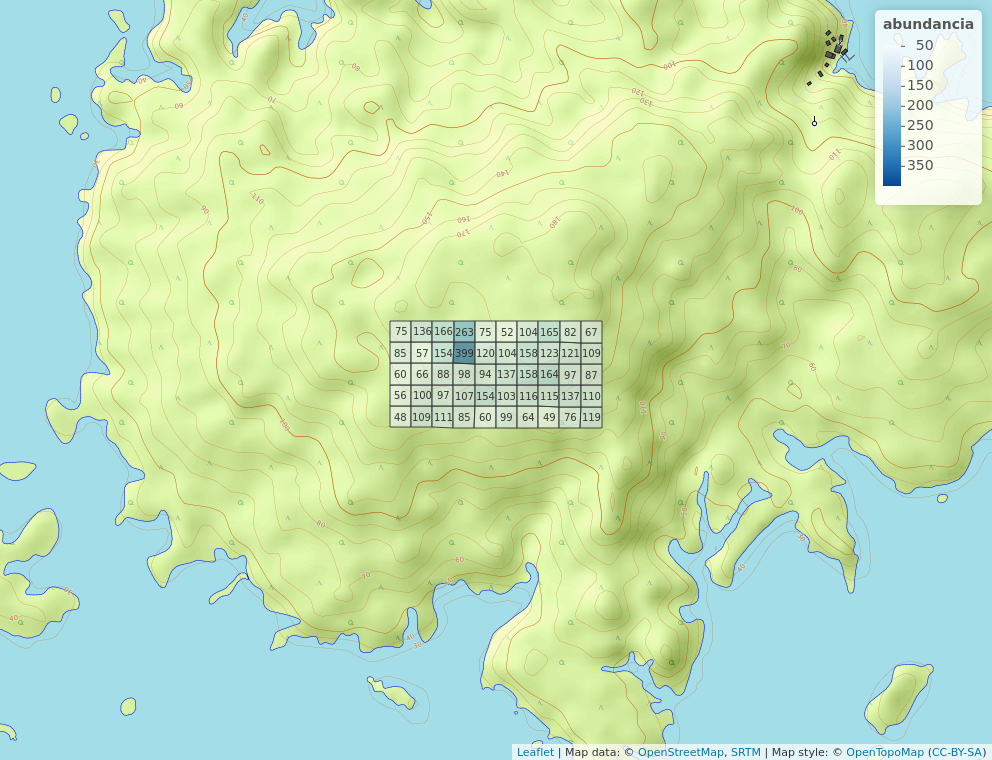
\includegraphics[width=0.80000\textwidth]{mapa_cuadros_abun_mi_familia.png}
\caption{Abundancia por cuadros de
\emph{Myrtaceae}.\label{fig:abumifam}}
\end{figure}

\begin{figure}
\centering
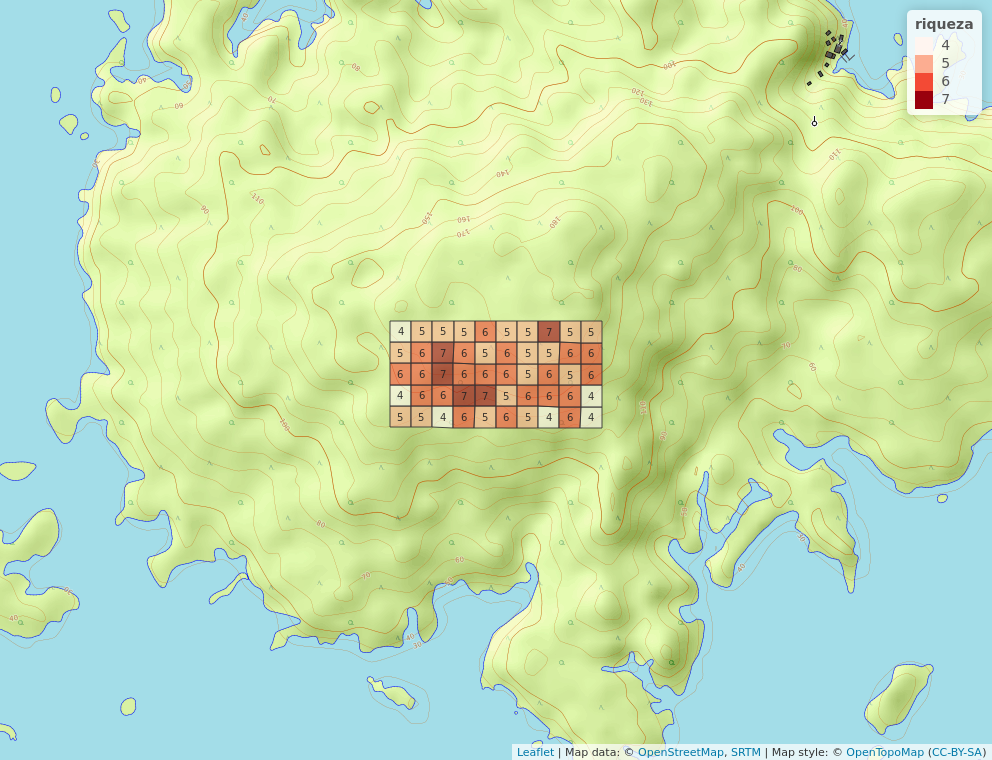
\includegraphics[width=0.80000\textwidth]{mapa_cuadros_riq_mi_familia.png}
\caption{Riqueza por cuadros de \emph{Myrtaceae}.\label{fig:riqmifam}}
\end{figure}

\begin{figure}
\centering
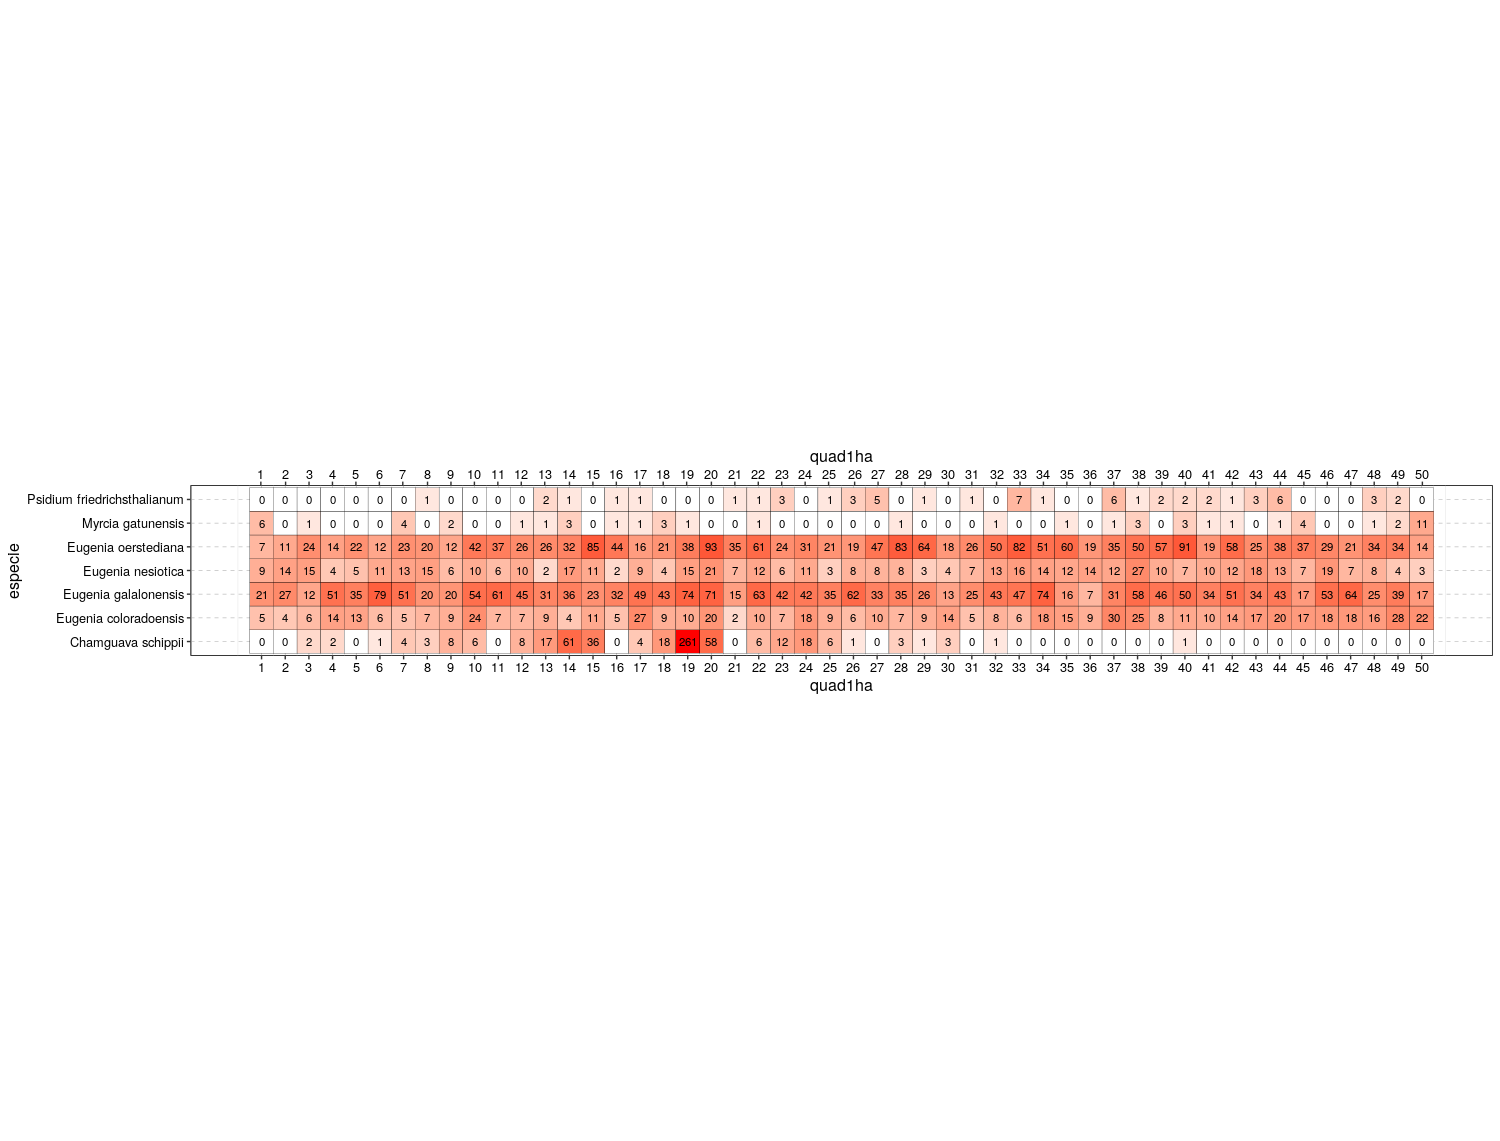
\includegraphics[width=1.00000\textwidth]{abuespecua.png}
\caption{Abundancia por especies por cuadros.\label{fig:abuxcua}}
\end{figure}

\begin{figure}
\centering
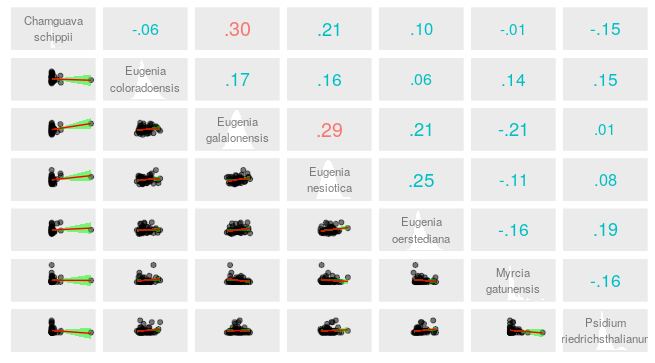
\includegraphics[width=0.70000\textwidth]{correlacion de pearson entre especies.png}
\caption{Matriz de correlación simple (Pearson) entre las especies de
\emph{Myrtaceae}.\label{fig:corresp}}
\end{figure}

\begin{figure}
\centering
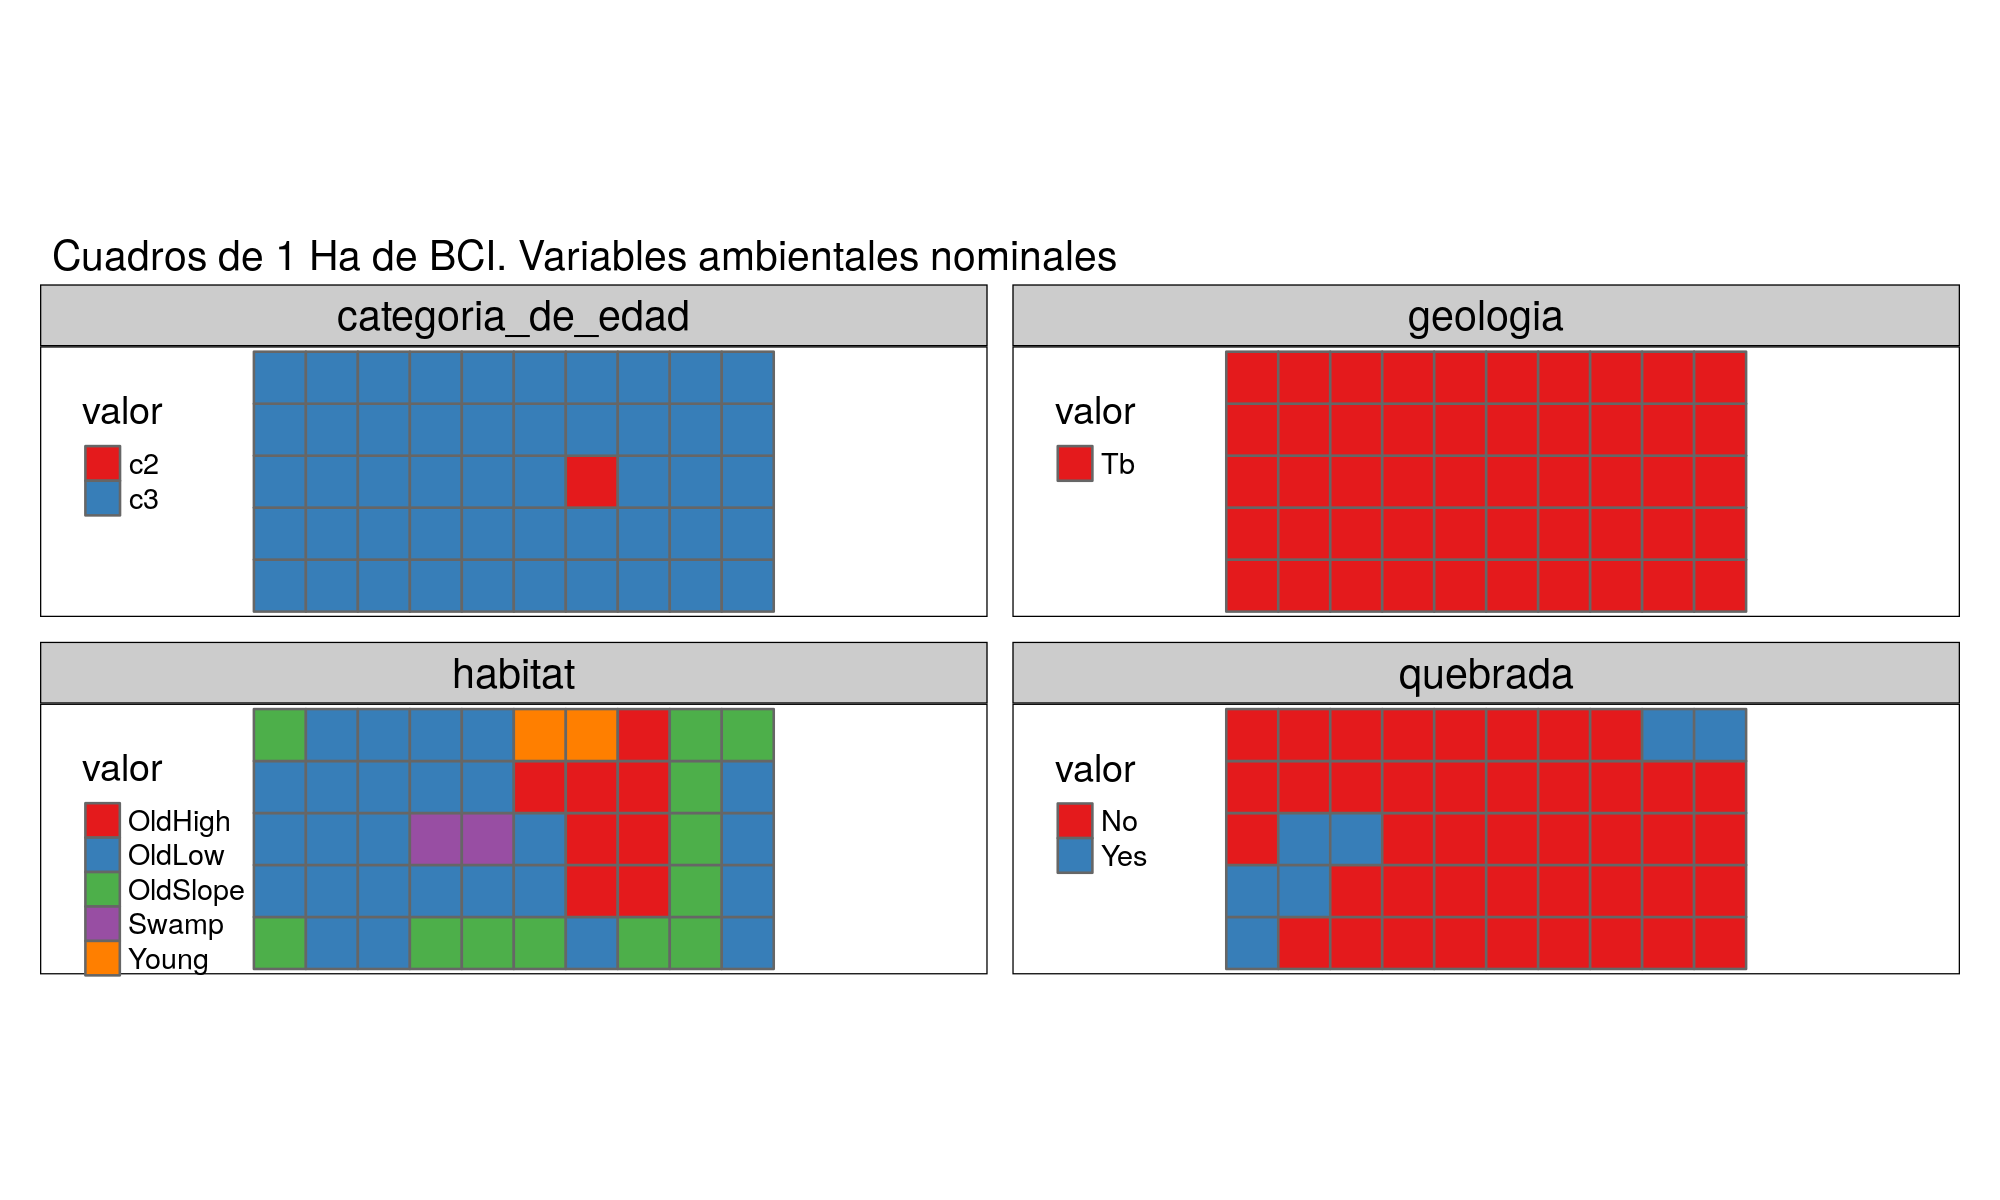
\includegraphics[width=0.90000\textwidth]{mapas_variables_ambientales_nominales_tmap.png}
\caption{Variables ambientales nominales.\label{fig:ambvar}}
\end{figure}

\begin{figure}
\centering
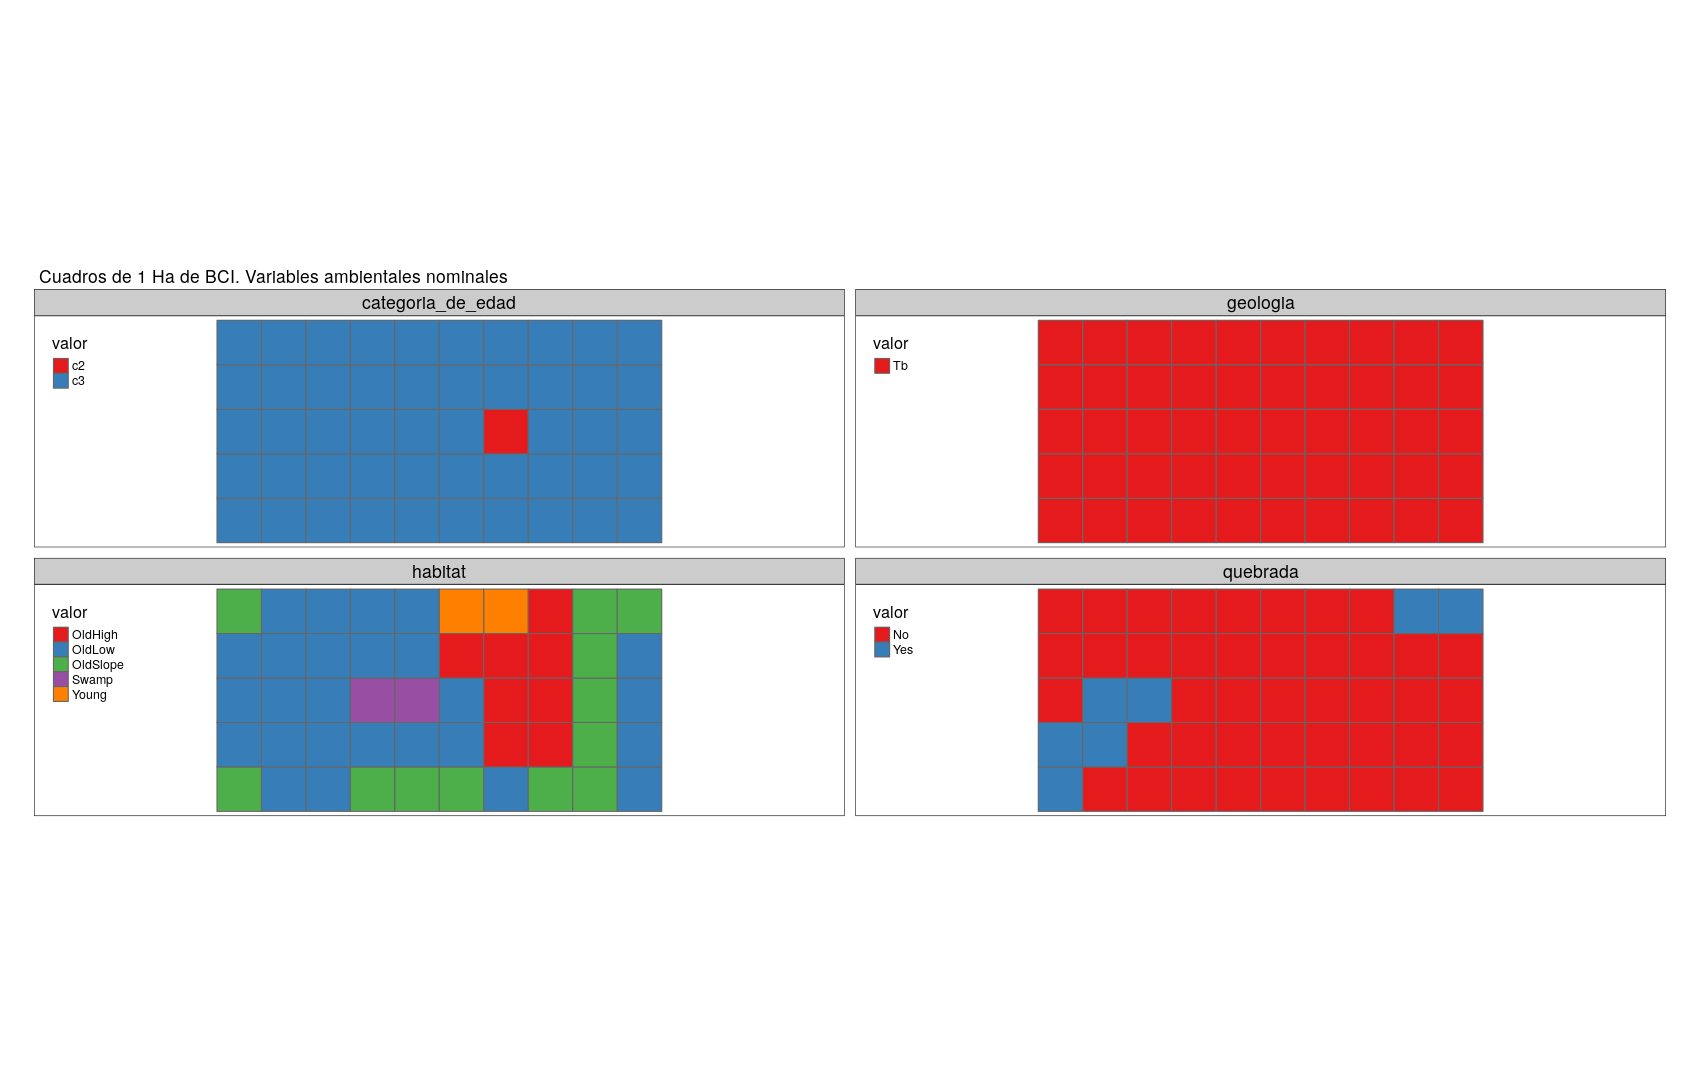
\includegraphics[width=1.00000\textwidth]{mapas_variables_ambientales_numericas.png}
\caption{Variables ambientales númericas.\label{fig:varnum}}
\end{figure}

\begin{figure}
\centering
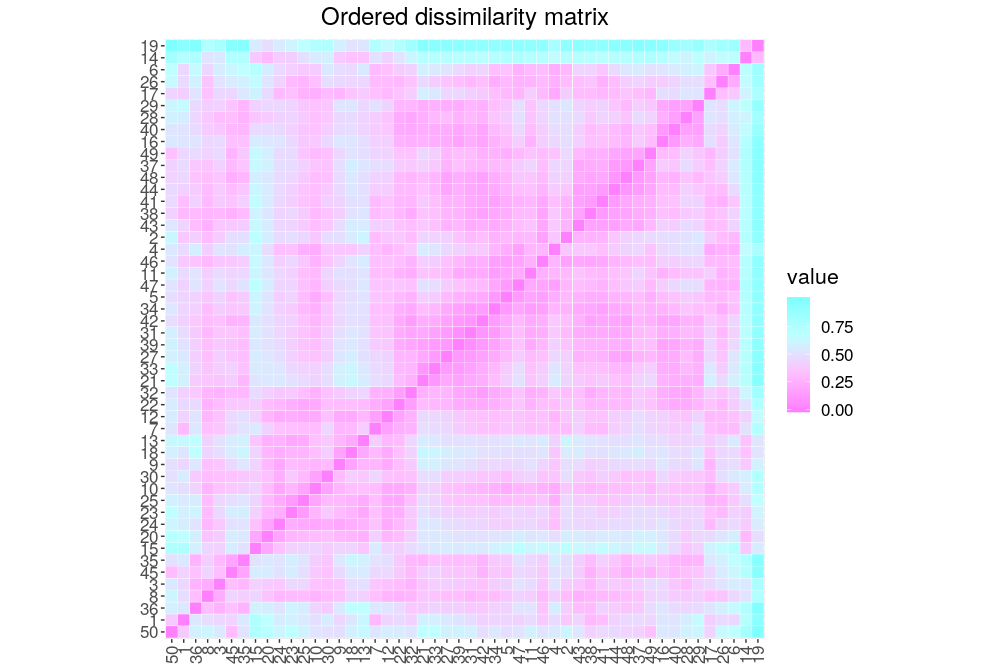
\includegraphics[width=1.00000\textwidth]{matriz de disimilaridad ordenada.png}
\caption{Matriz de asociación de sitios en la parcela de BCI. El color
fucsia o rosa indica una corta distancia o que son muy similares los
sitios, y el celeste indica una gran distancia o que los sitios son poco
similares.\label{fig:matrizdisimord}}
\end{figure}

\begin{figure}
\centering
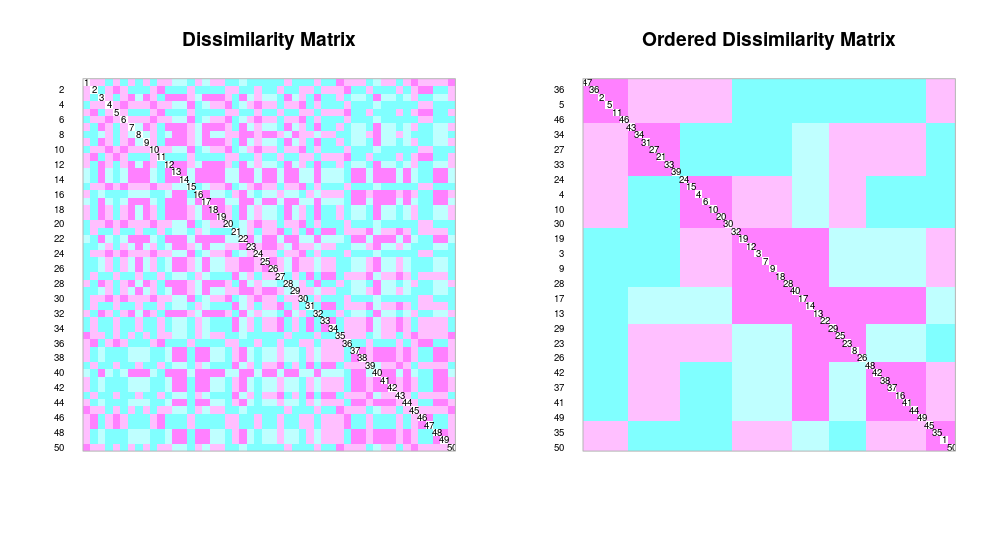
\includegraphics[width=1.00000\textwidth]{matriz de disimilaridad de jaccard.png}
\caption{Matriz de disimilaridad de Jaccard. El color fucsia o rosa
indica una corta distancia o que son muy similares los sitios, y el
celeste indica una gran distancia o que los sitios son poco
similares.\label{fig:matrizjacc}}
\end{figure}

\begin{figure}
\centering
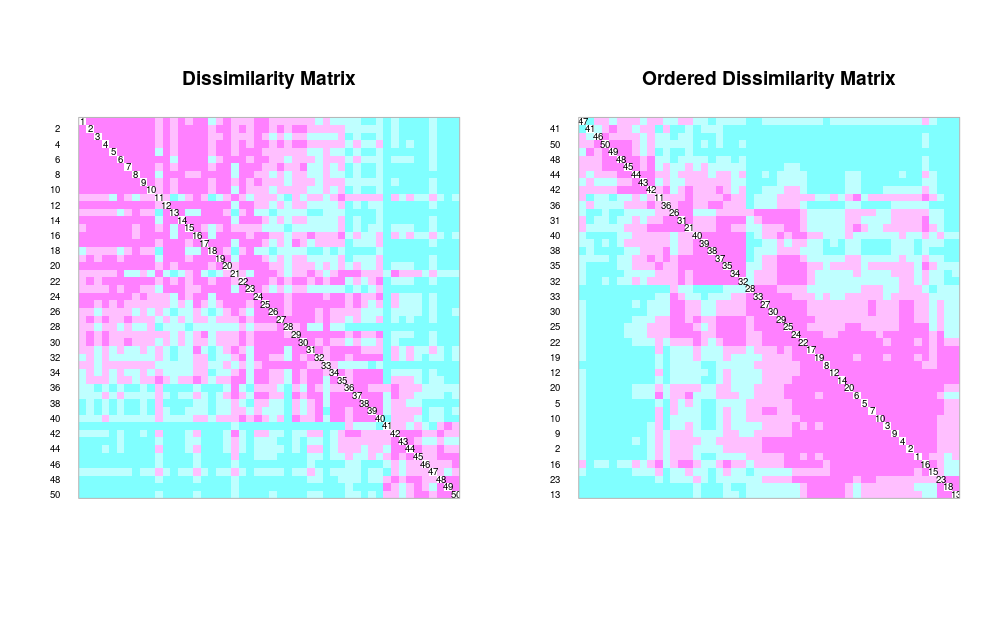
\includegraphics[width=1.00000\textwidth]{variables de suelo_disimilaridad.png}
\caption{Matriz de disimilaridad de las variables edáficas en la parcela
de BCI. El color fucsia o rosa indica una corta distancia o que son muy
similares los sitios, y el celeste indica una gran distancia o que los
sitios son poco similares.\label{fig:suelodis}}
\end{figure}

\begin{figure}
\centering
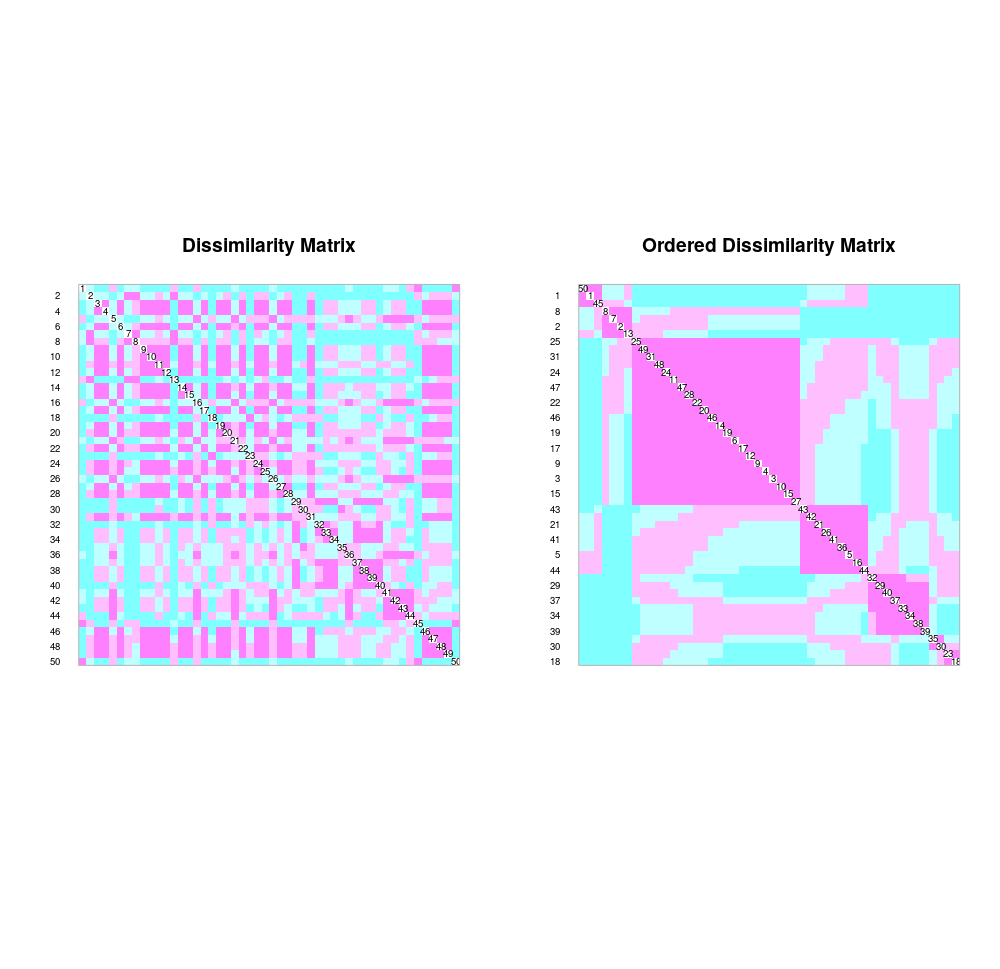
\includegraphics[width=1.00000\textwidth]{Variables mixtas.png}
\caption{Matriz de disimilaridad de variables mixtas
(\texttt{heterogeneidadambiental}, \texttt{hábitat} y
\texttt{quebrada}). El color fucsia o rosa indica una corta distancia o
que son muy similares los sitios, y el celeste indica una gran distancia
o que los sitios son poco similares.\label{fig:mixtadis}}
\end{figure}

\begin{figure}
\centering
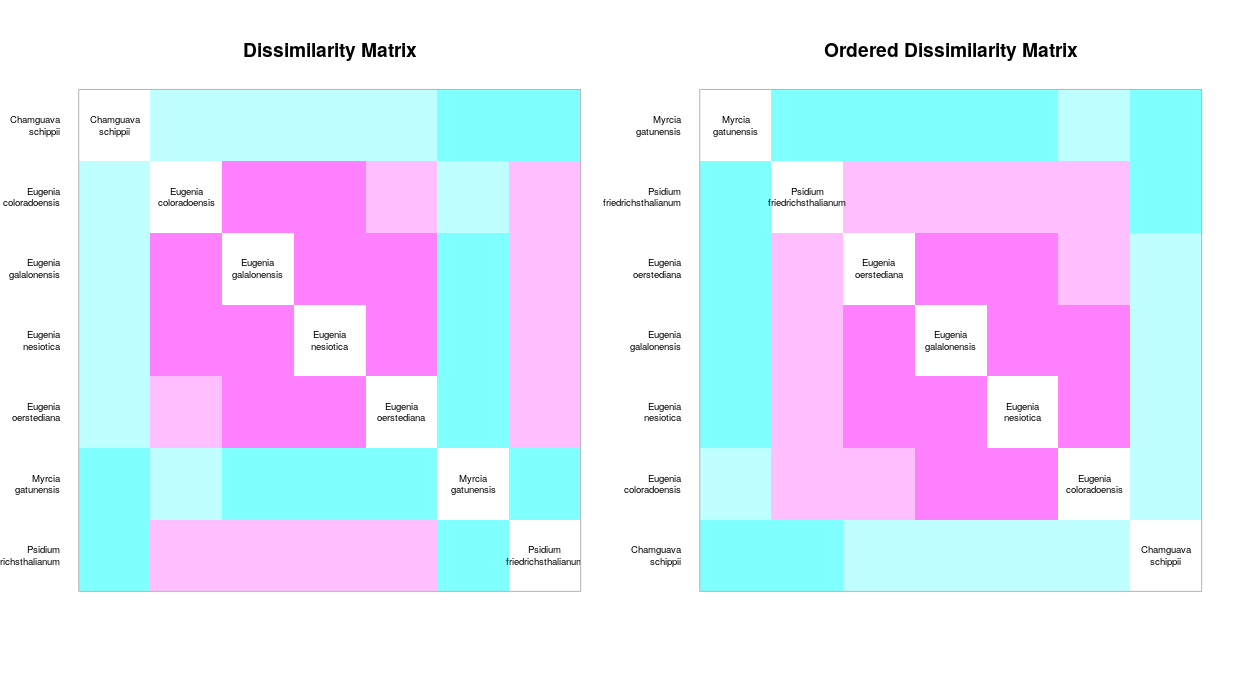
\includegraphics[width=1.00000\textwidth]{dependencia_especies.png}
\caption{Mapa de asociación entre especies según la abundancia. El color
rosa indica que existe dependencia y el azul que no existe de
dependencia.\label{fig:asoespec}}
\end{figure}

\begin{figure}
\centering
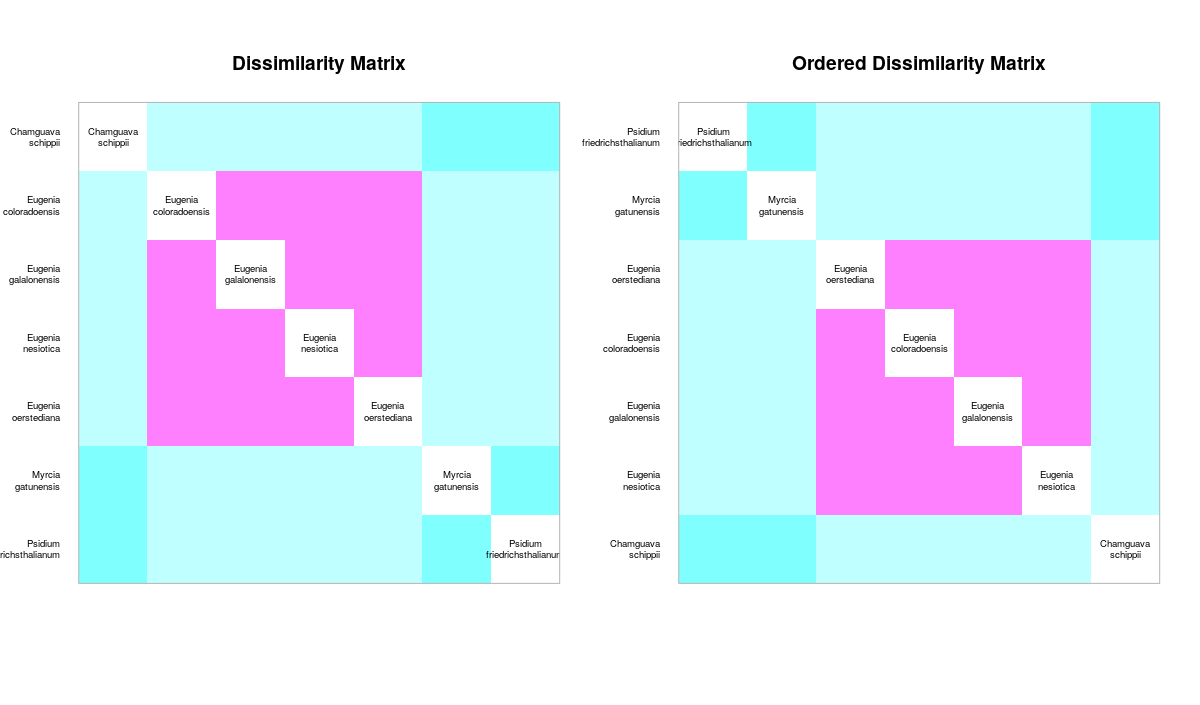
\includegraphics[width=1.00000\textwidth]{depn_espc_jacc.png}
\caption{Mapa de dependencia entre especies según datos de
presencia/ausencia. El color rosa indica que existe dependencia y el
azul que no existe de dependencia.\label{fig:dependenciajacc}}
\end{figure}

\begin{figure}
\centering
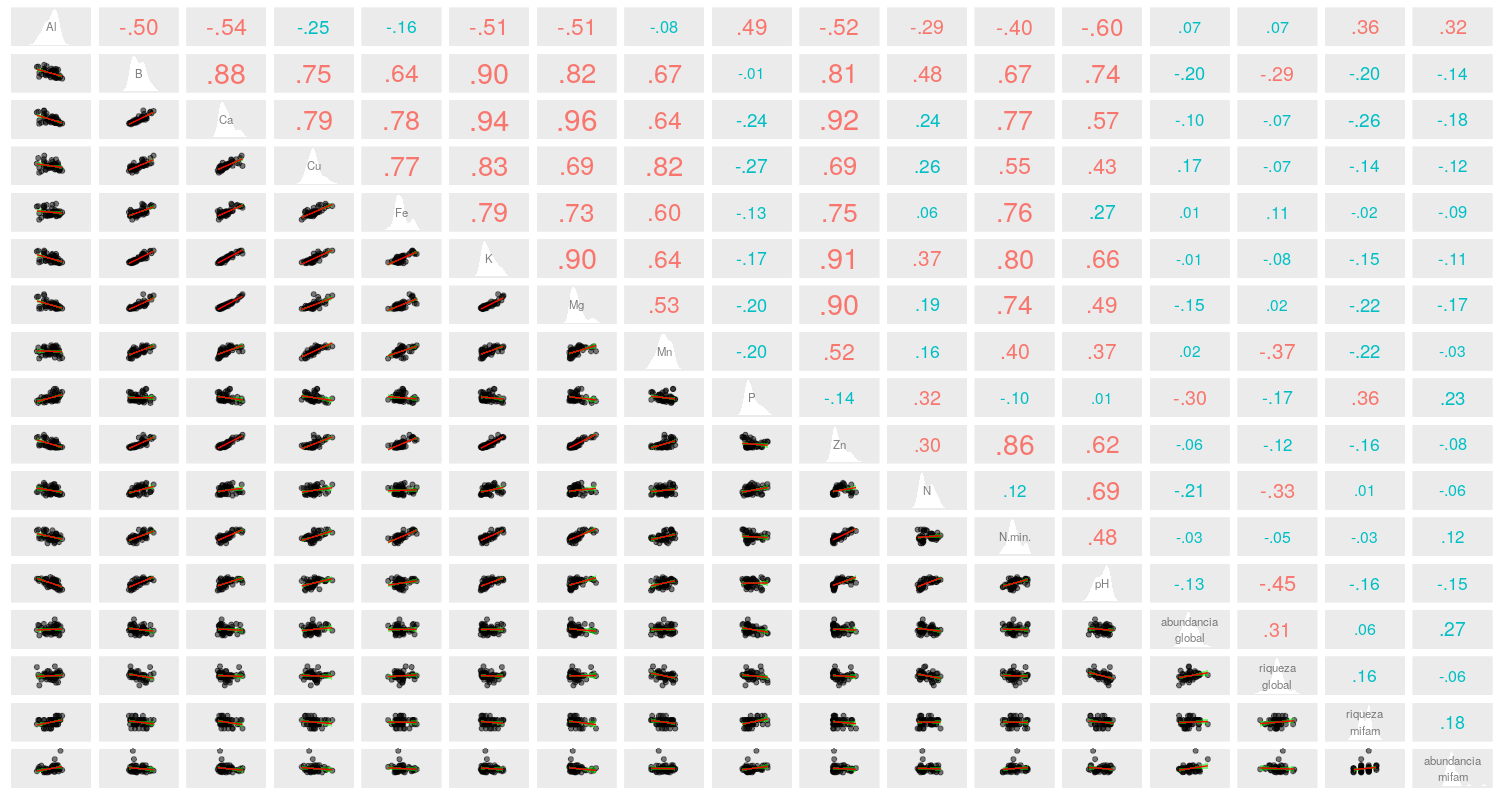
\includegraphics[width=1.00000\textwidth]{Chi_var_edaf_asoc_R.png}
\caption{Matriz de correlación de Pearson, asociación entre riqueza y
abundacia de \emph{Myrtaceae} y las variables
edáficas.\label{fig:chivardep}}
\end{figure}

\begin{figure}
\centering
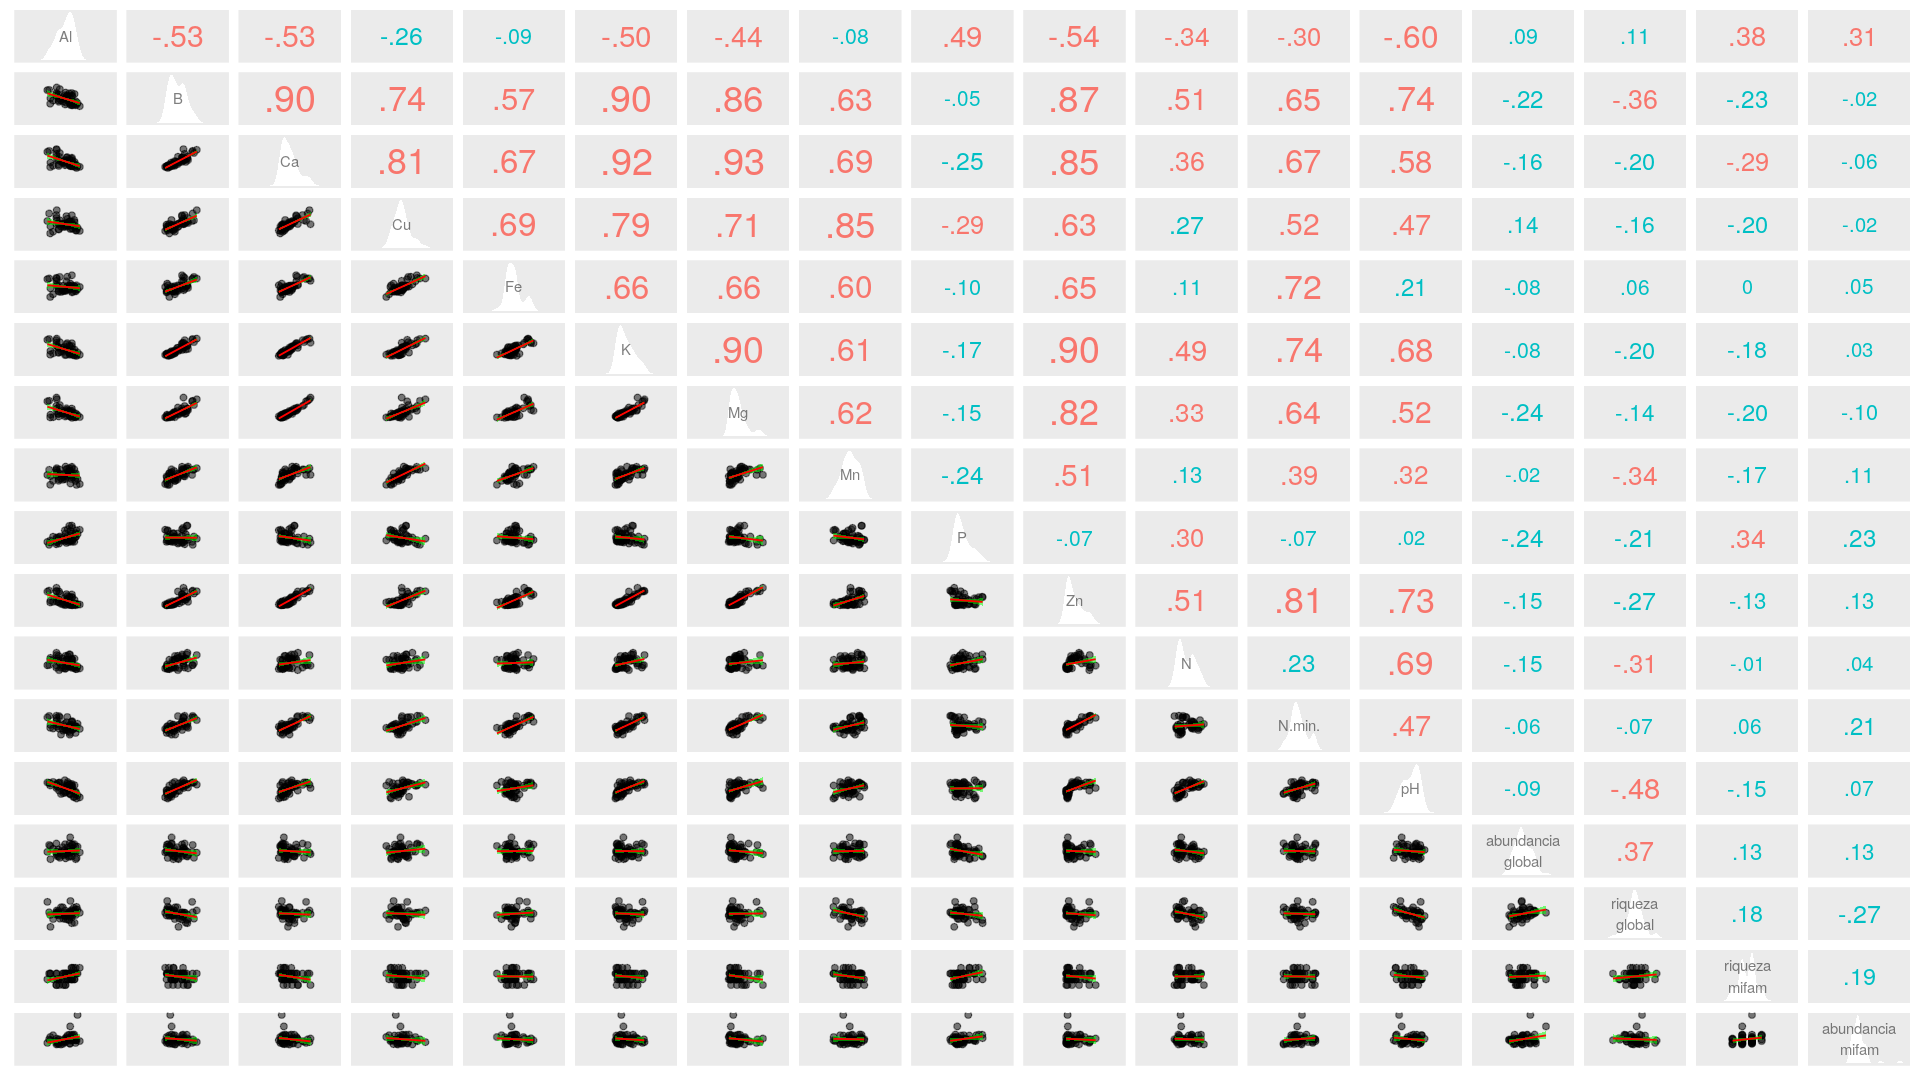
\includegraphics[width=1.00000\textwidth]{matriz_correlacion_suelo_abun_riq_spearman.png}
\caption{Matriz de Spearman, asociación entre riqueza y abundancia de
\emph{Myrtaceae} con las variables edáficas.\label{fig:mspearman}}
\end{figure}

\begin{figure}
\centering
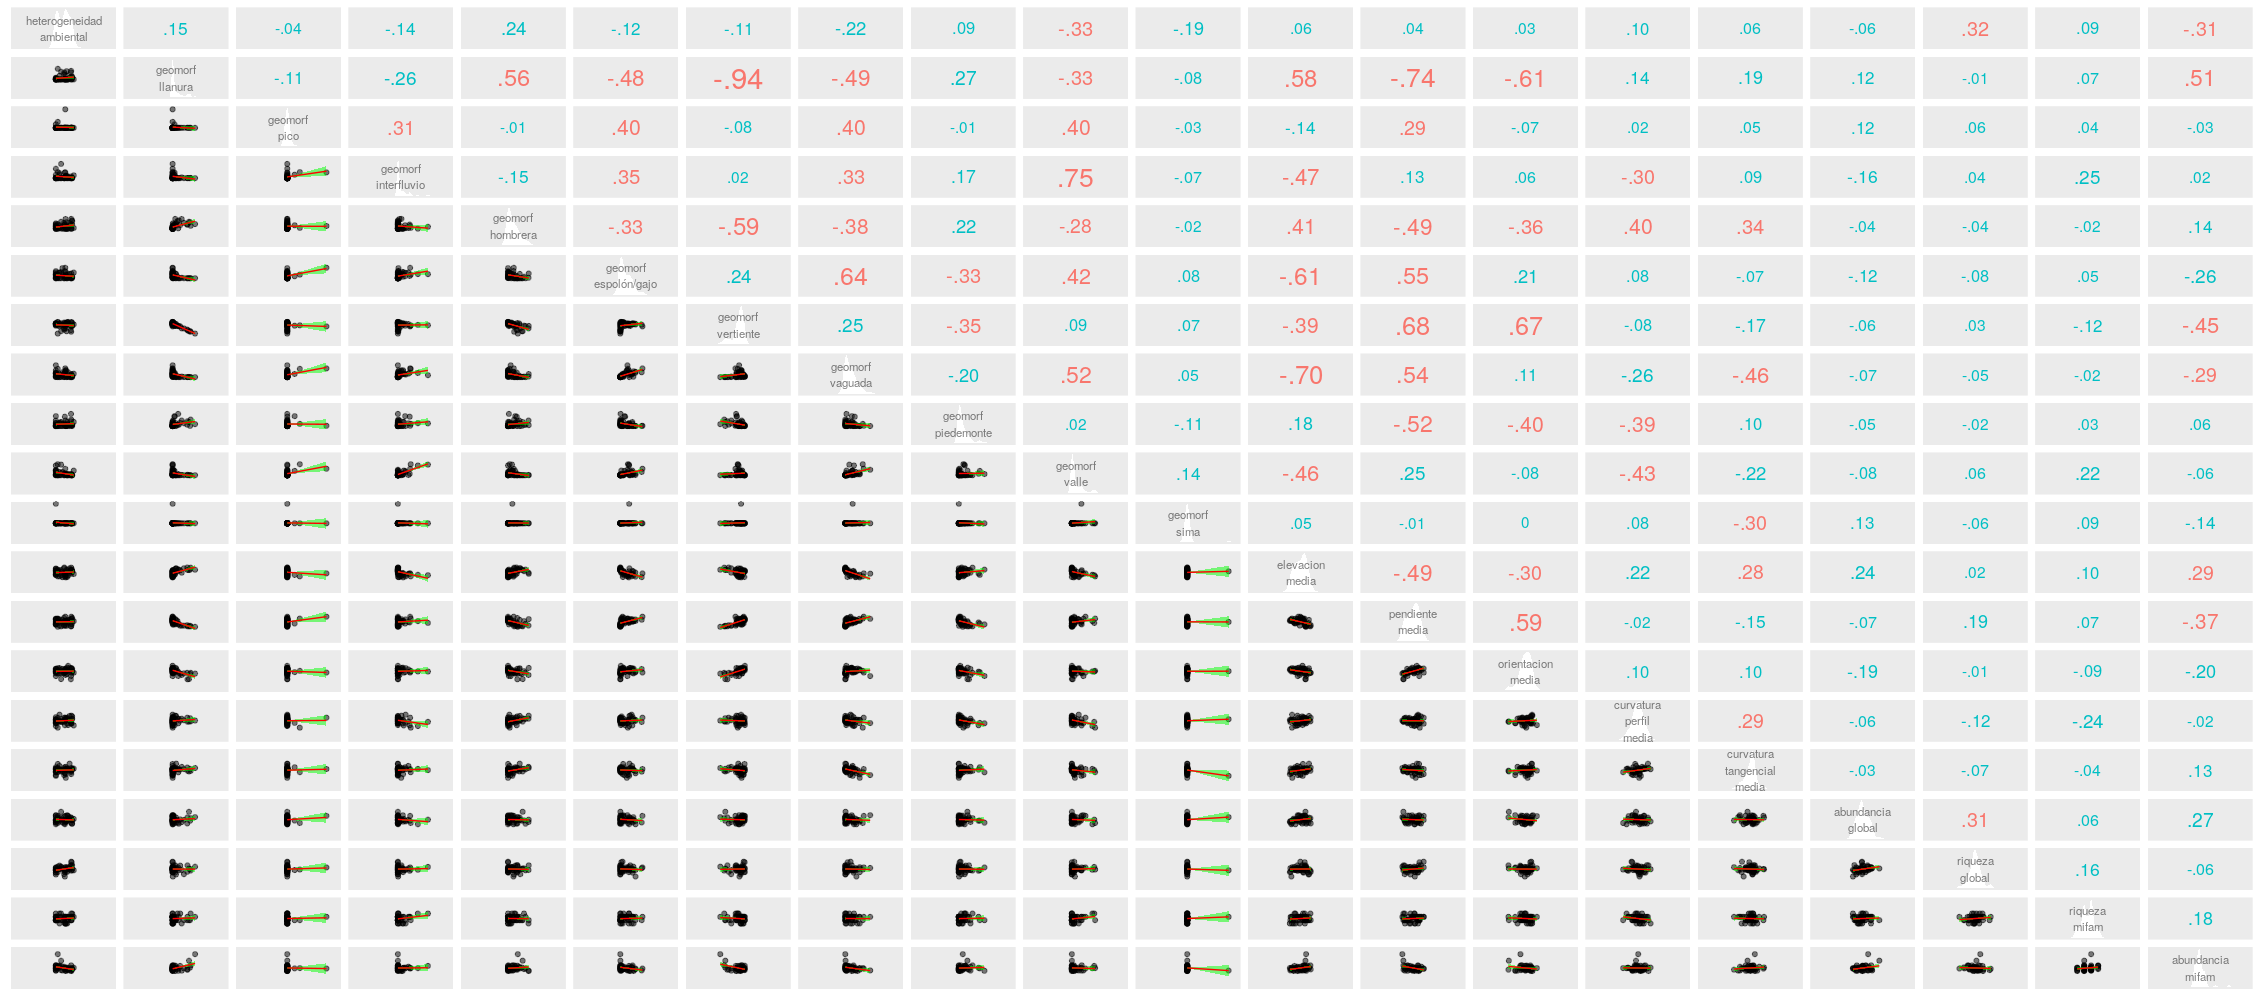
\includegraphics[width=1.00000\textwidth]{Matriz_correlacion_pearson.png}
\caption{Matriz de Pearson, asociación entre riqueza y abundancia de
\emph{Myrtaceae} y las variables
geomorfológicas.\label{fig:pearson_geom}}
\end{figure}

\begin{figure}
\centering
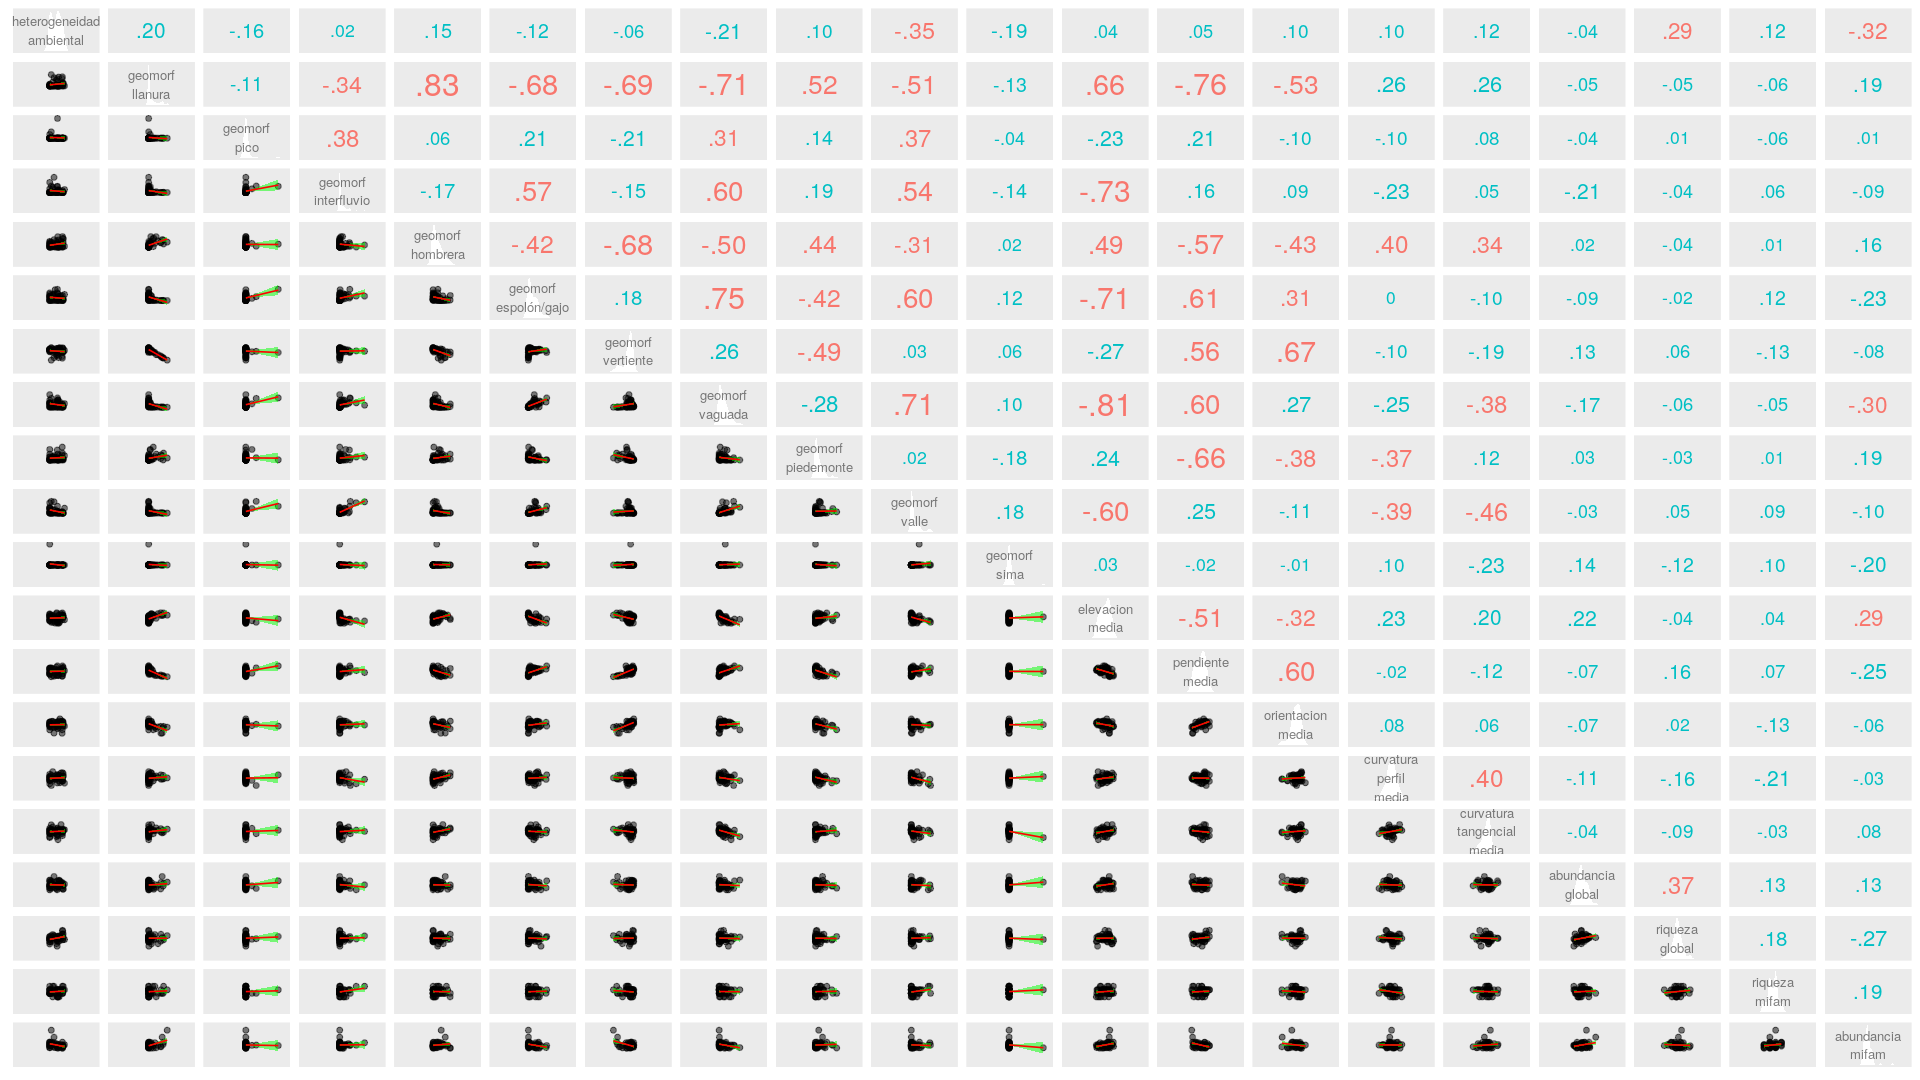
\includegraphics[width=1.00000\textwidth]{matriz_correlacion_geomorf_abun_riq_spearman.png}
\caption{Matriz de Spearman, asociación entre riqueza y abundancia de
\emph{Myrtaceae} y las variables
geomorfológicas.\label{fig:spearm_geom}}
\end{figure}

\begin{figure}
\centering
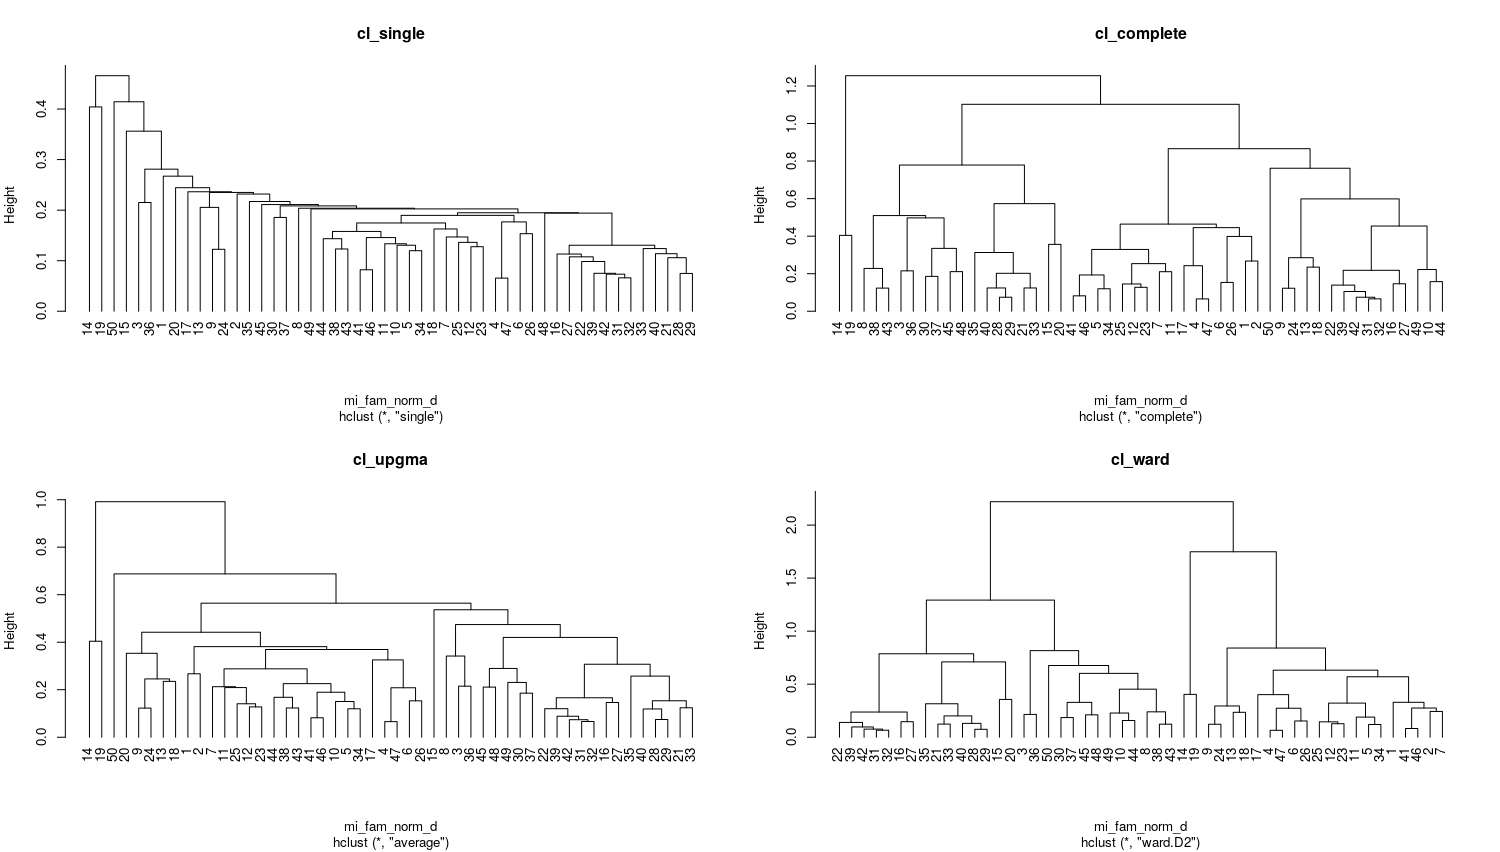
\includegraphics[width=1.00000\textwidth]{meth_enl.png}
\caption{Dendrogramas a partir criterios de enlaces simple, completo y
por promedio (UPGMA) y Ward o varianza mínima,\label{fig:enlaces}}
\end{figure}

\begin{figure}
\centering
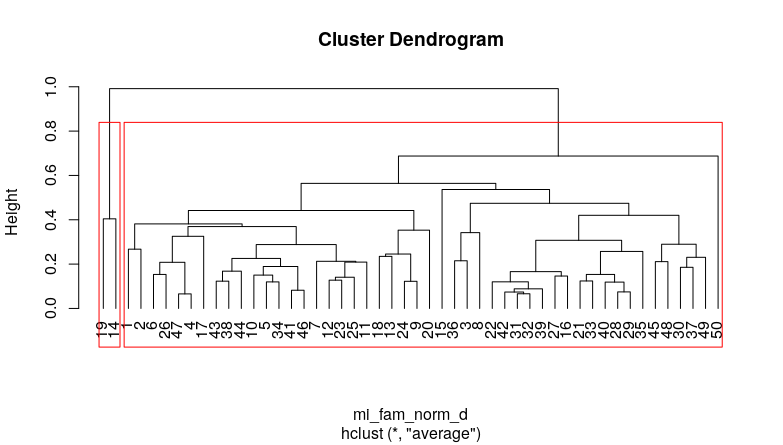
\includegraphics[width=0.50000\textwidth]{2UPGMA den.png}
\caption{Dendrograma de grupo optimo según el criterio de enlace
UPGMA.\label{fig:upgmaden}}
\end{figure}

\begin{figure}
\centering
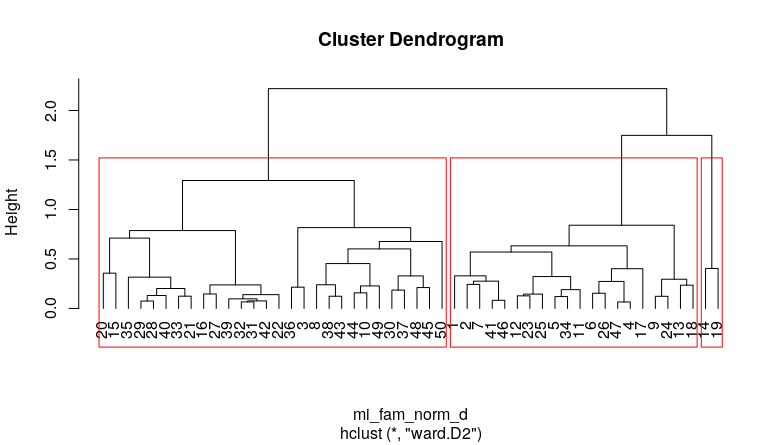
\includegraphics[width=0.50000\textwidth]{ward_den.png}
\caption{Dendrograma según criterio de enlace Ward.\label{fig:wardden}}
\end{figure}

\begin{figure}
\centering
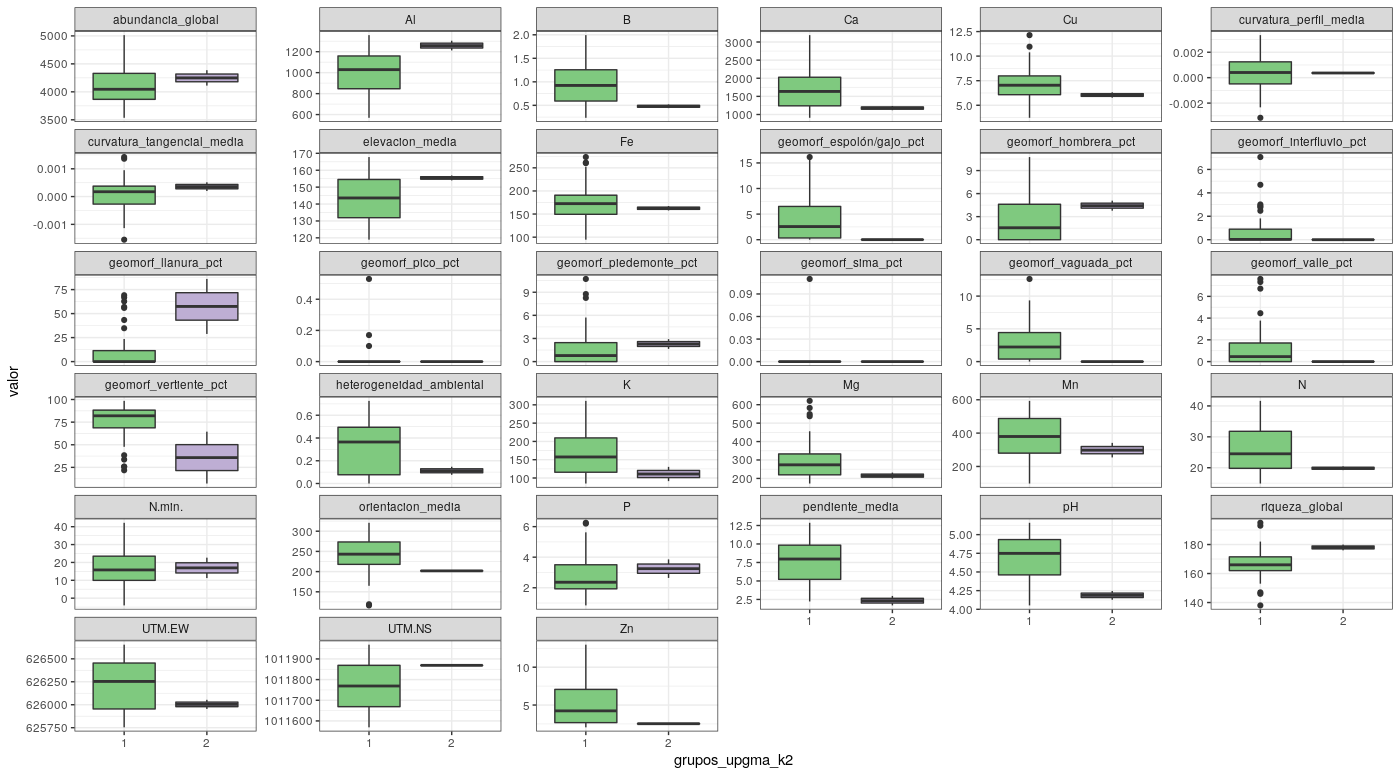
\includegraphics[width=0.70000\textwidth]{caja_upgma.png}
\caption{Diagramas de caja de las variables ambientales en los grupos de
UPGMA.\label{fig:upgma_caja}}
\end{figure}

\begin{figure}
\centering
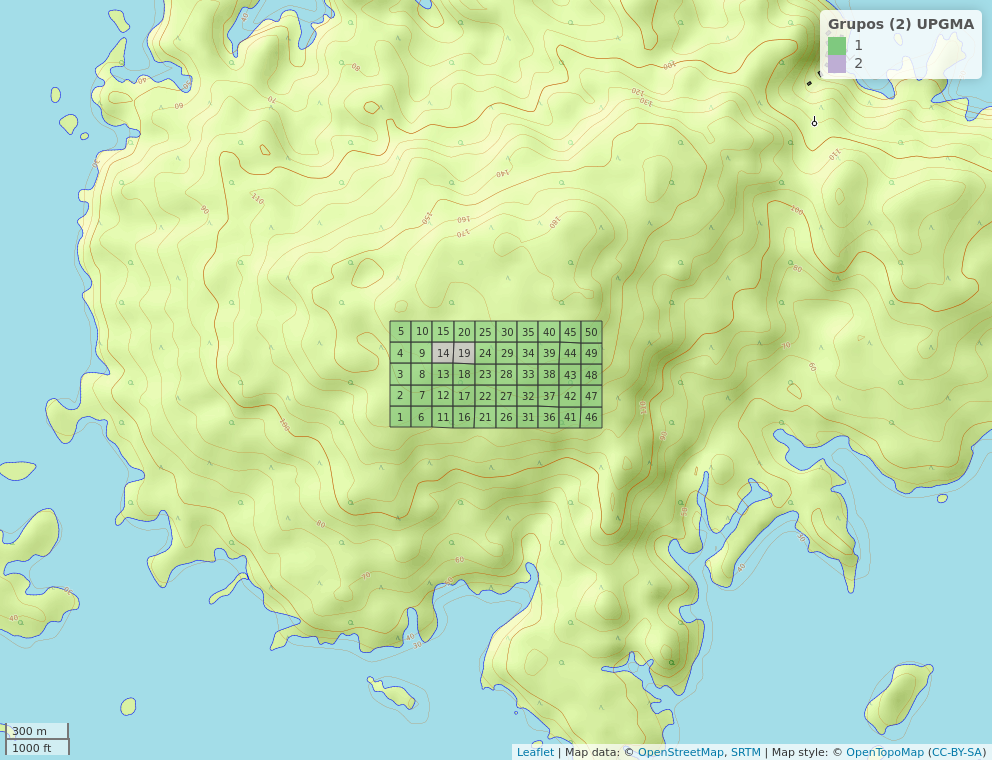
\includegraphics[width=0.60000\textwidth]{mapa_upgma_k2.png}
\caption{Mapa de los grupos formados por el criterio de enlace UPGMA.
\label{fig:gruposU}}
\end{figure}

\begin{figure}
\centering
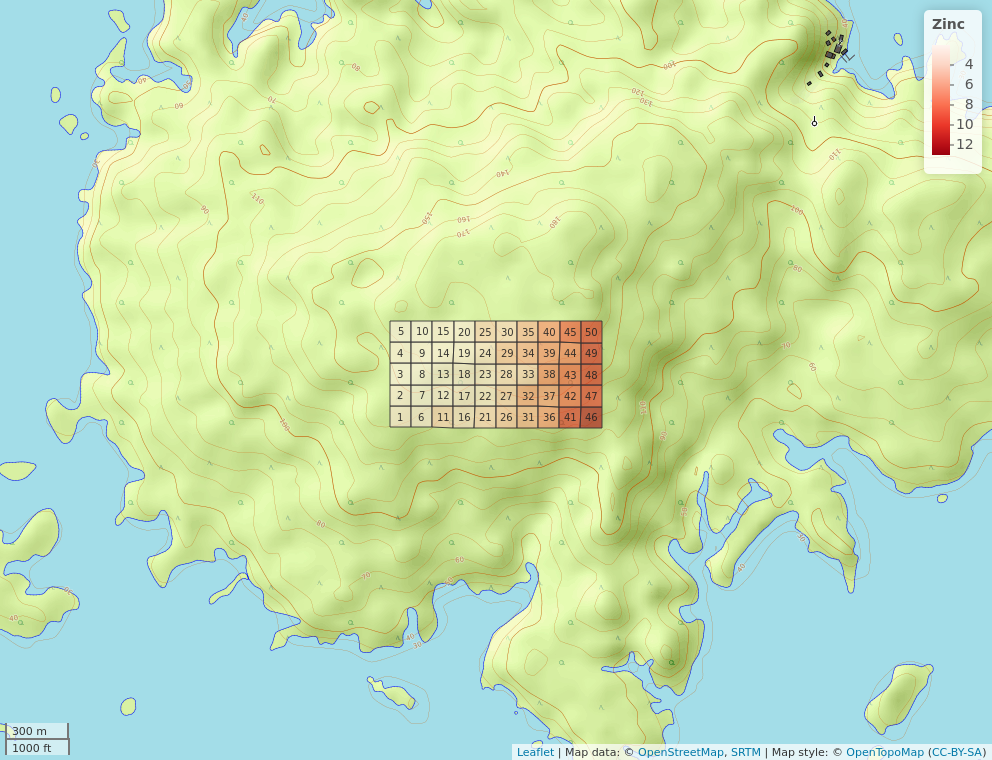
\includegraphics[width=0.60000\textwidth]{mapa_zinc.png}
\caption{Mapa de concentración de zinc en los sitios de la parcela de
BCI.\label{fig:zinc}}
\end{figure}

\begin{figure}
\centering
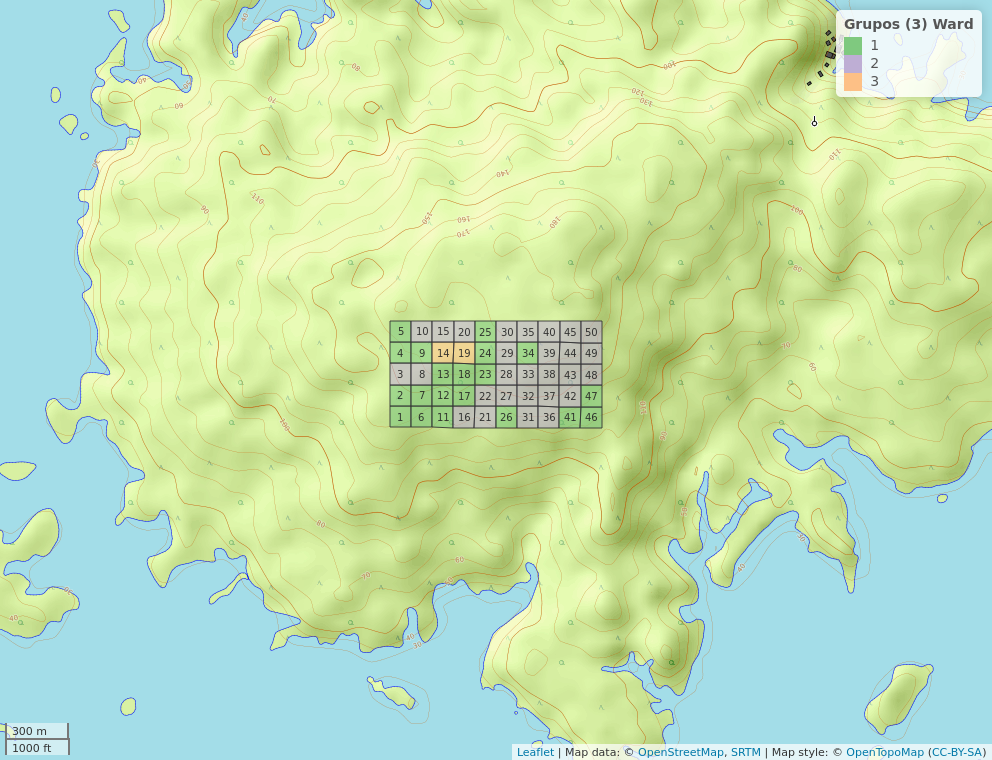
\includegraphics[width=0.60000\textwidth]{mapa_ward_k3.png}
\caption{Mapa de los grupos formados por el criterio de enlace Ward.
\label{fig:gruposW}}
\end{figure}

\begin{figure}
\centering
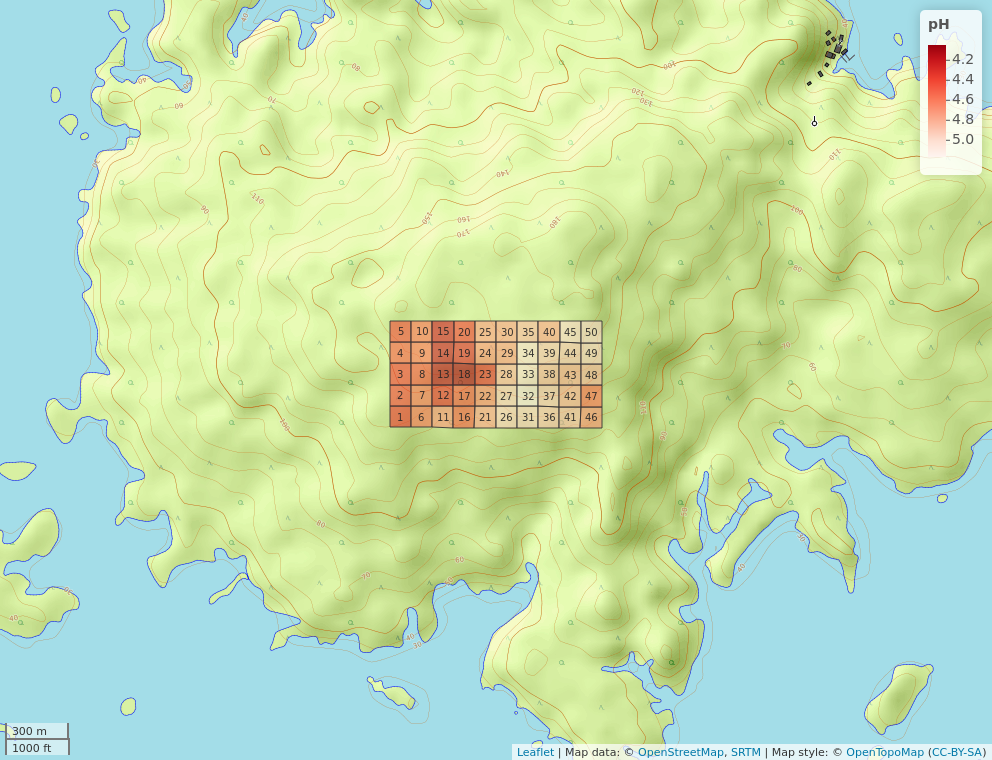
\includegraphics[width=0.60000\textwidth]{mapa_ph.png}
\caption{Mapa de concentración de pH en los sitios de la parcela de
BCI.\label{fig:ph}}
\end{figure}

\begin{figure}
\centering
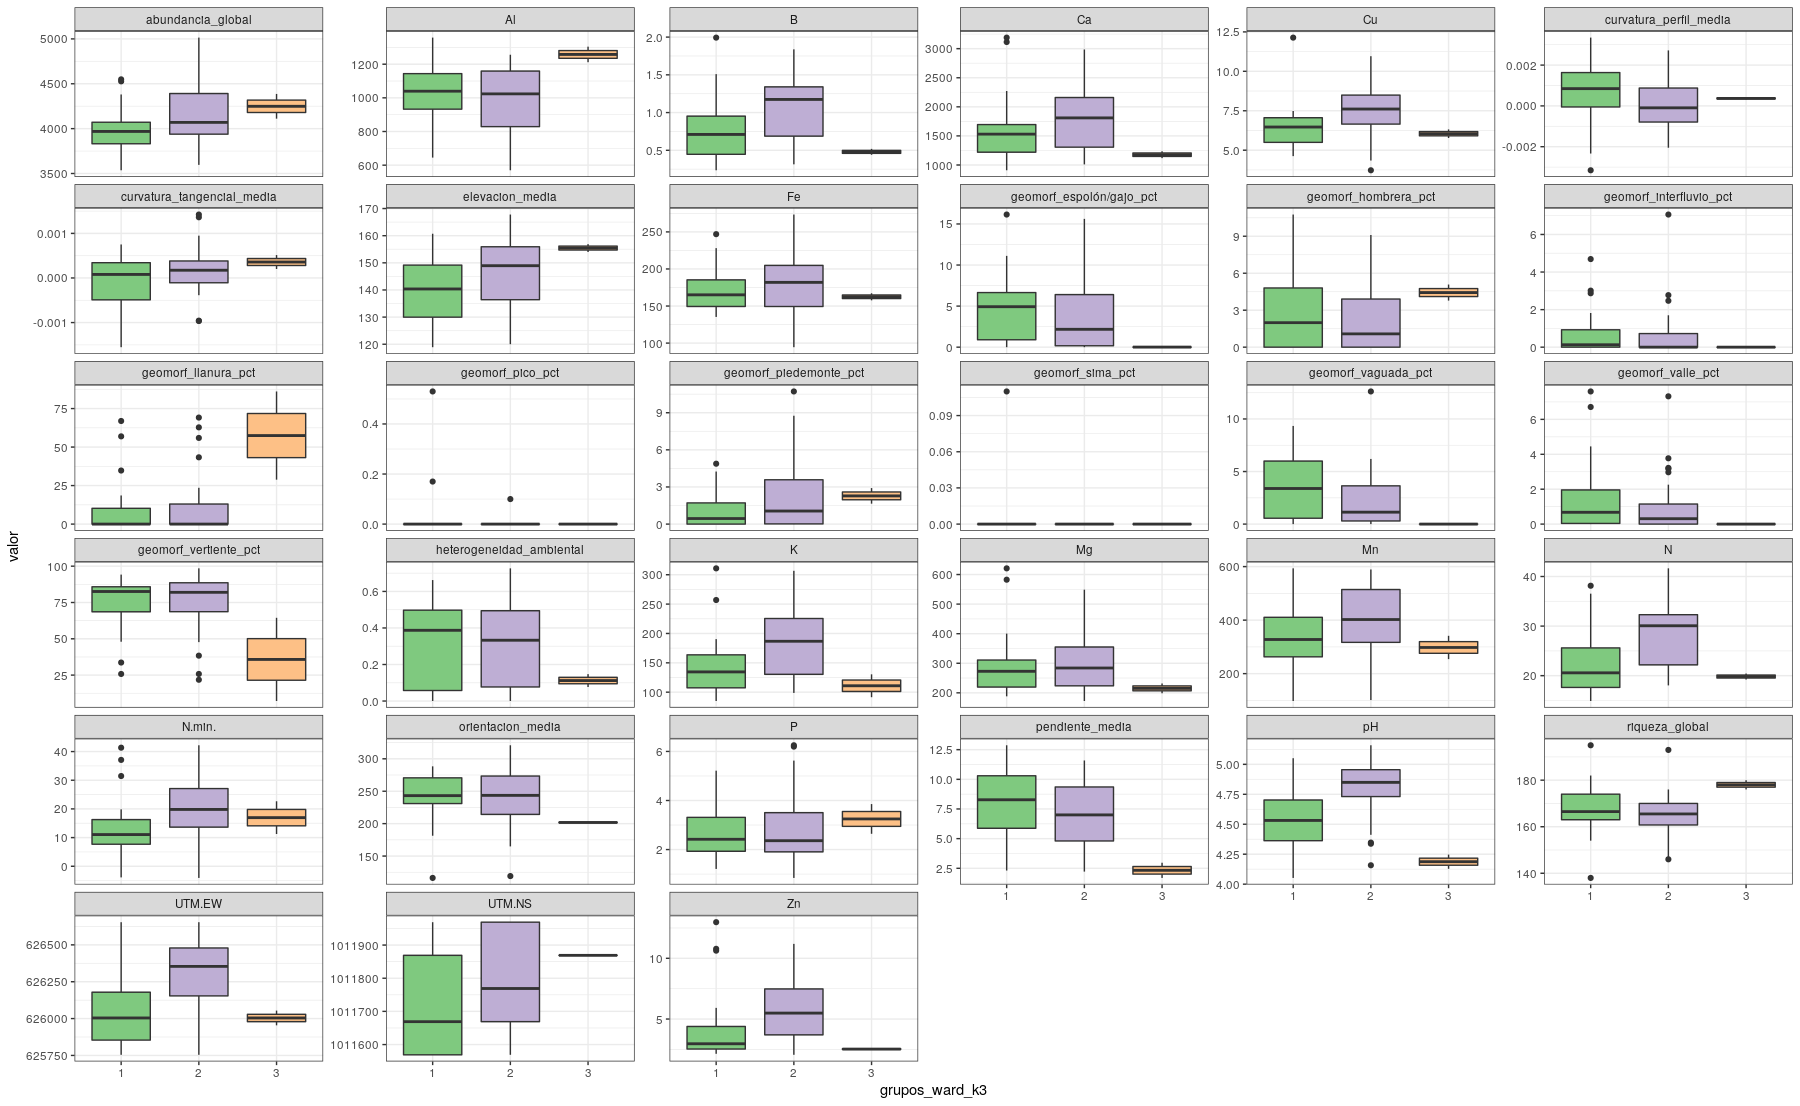
\includegraphics[width=0.70000\textwidth]{ward_caja.png}
\caption{Diagramas de caja de las variables ambientales en los grupos de
Ward.\label{fig:ward_caja}}
\end{figure}

\begin{figure}
\centering
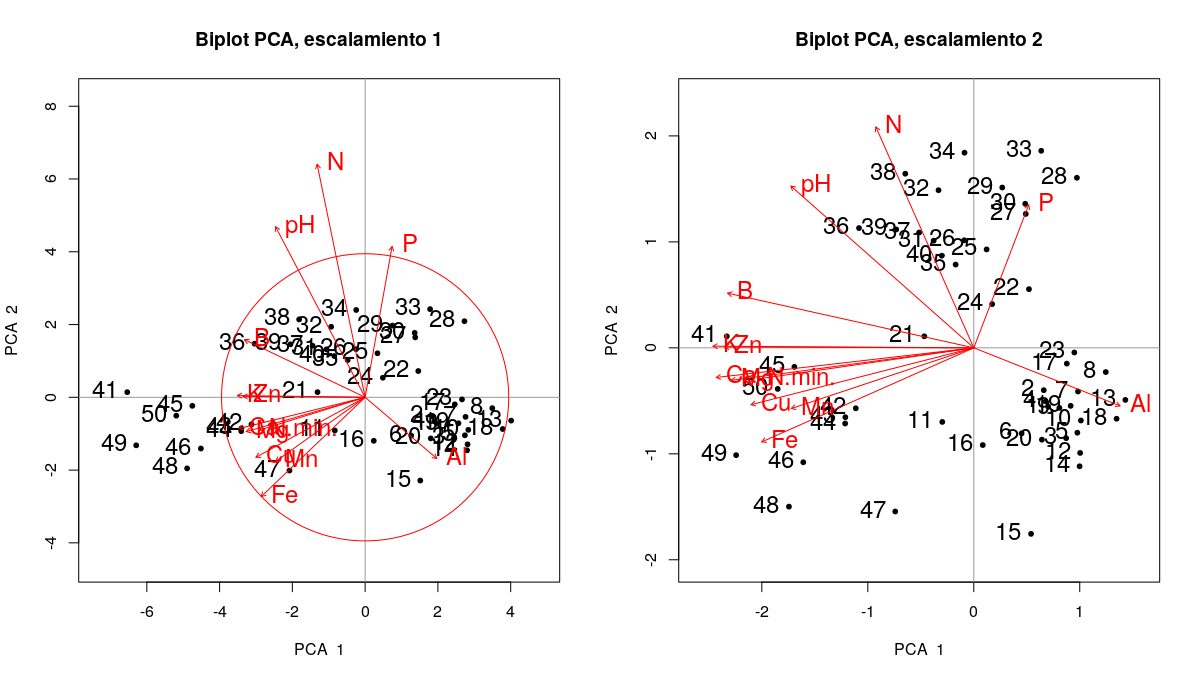
\includegraphics[width=0.80000\textwidth]{escalamiento_ward.png}
\caption{Distribución de sitios y variables de suelo en
Biplot.\label{fig:escalamientobi}}
\end{figure}

\begin{figure}
\centering
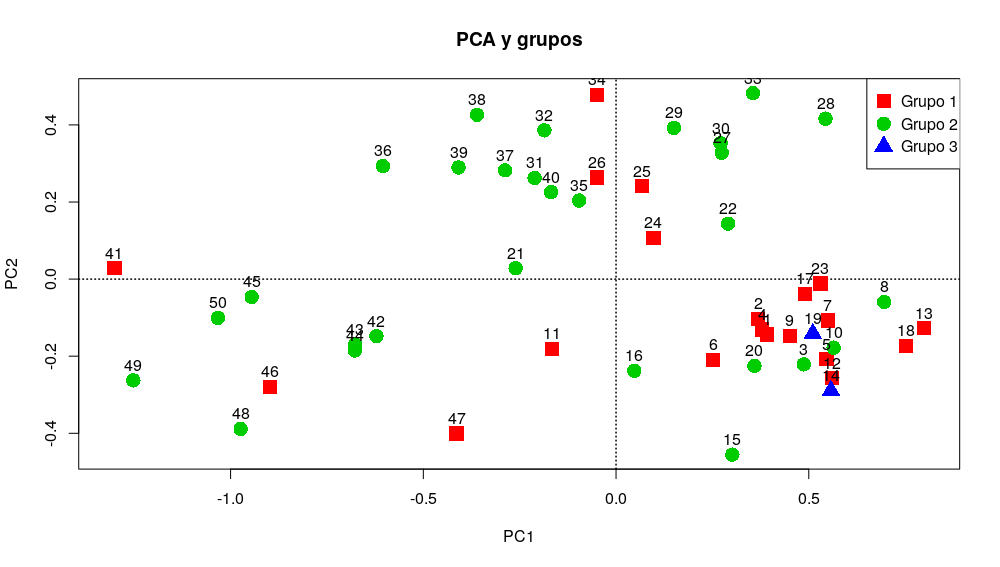
\includegraphics[width=0.60000\textwidth]{biplot upgma.png}
\caption{Distribución de sitios por grupos de
puntuaciones.\label{fig:upgmabip}}
\end{figure}

\begin{figure}
\centering
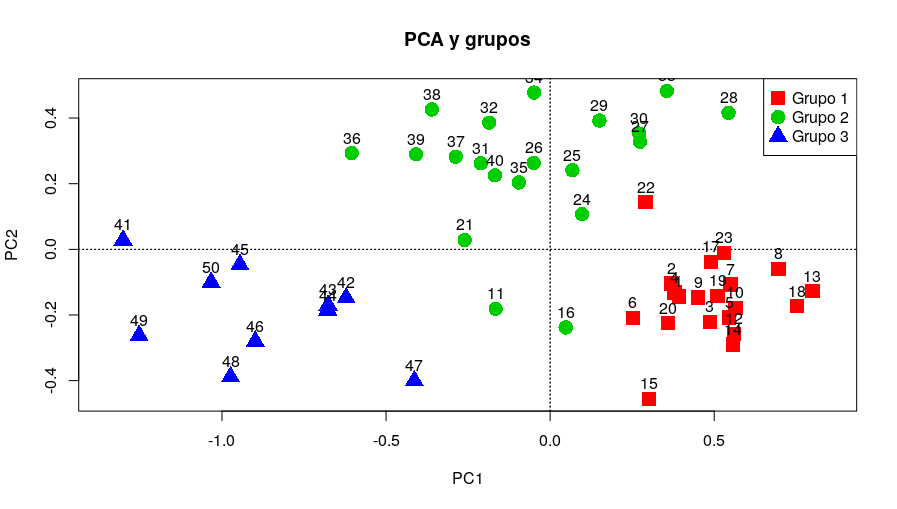
\includegraphics[width=0.50000\textwidth]{grafico de cluste PCA.png}
\caption{Distribución de sitios de los grupos UPGMA según puntuaciones
(PCA).\label{fig:puntuaciones}}
\end{figure}

\begin{figure}
\centering
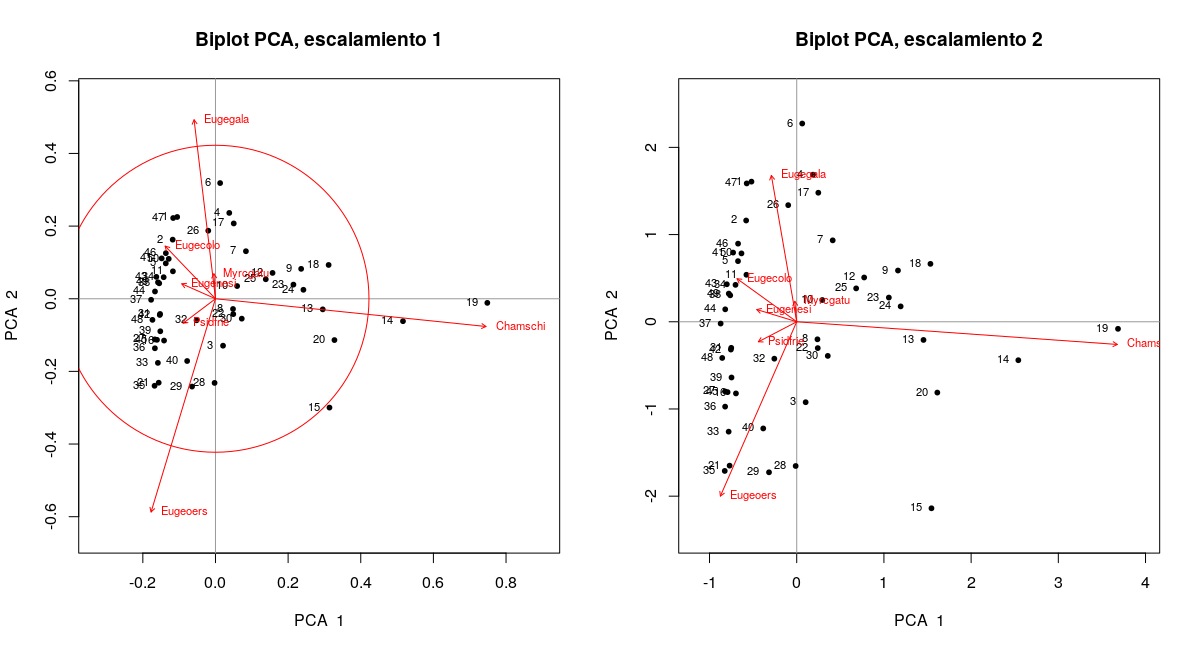
\includegraphics[width=0.50000\textwidth]{pca com amb.png}
\caption{Distribución de especies según su contribución a los sitio
(PCA).\label{fig:paccont}}
\end{figure}

\begin{figure}
\centering
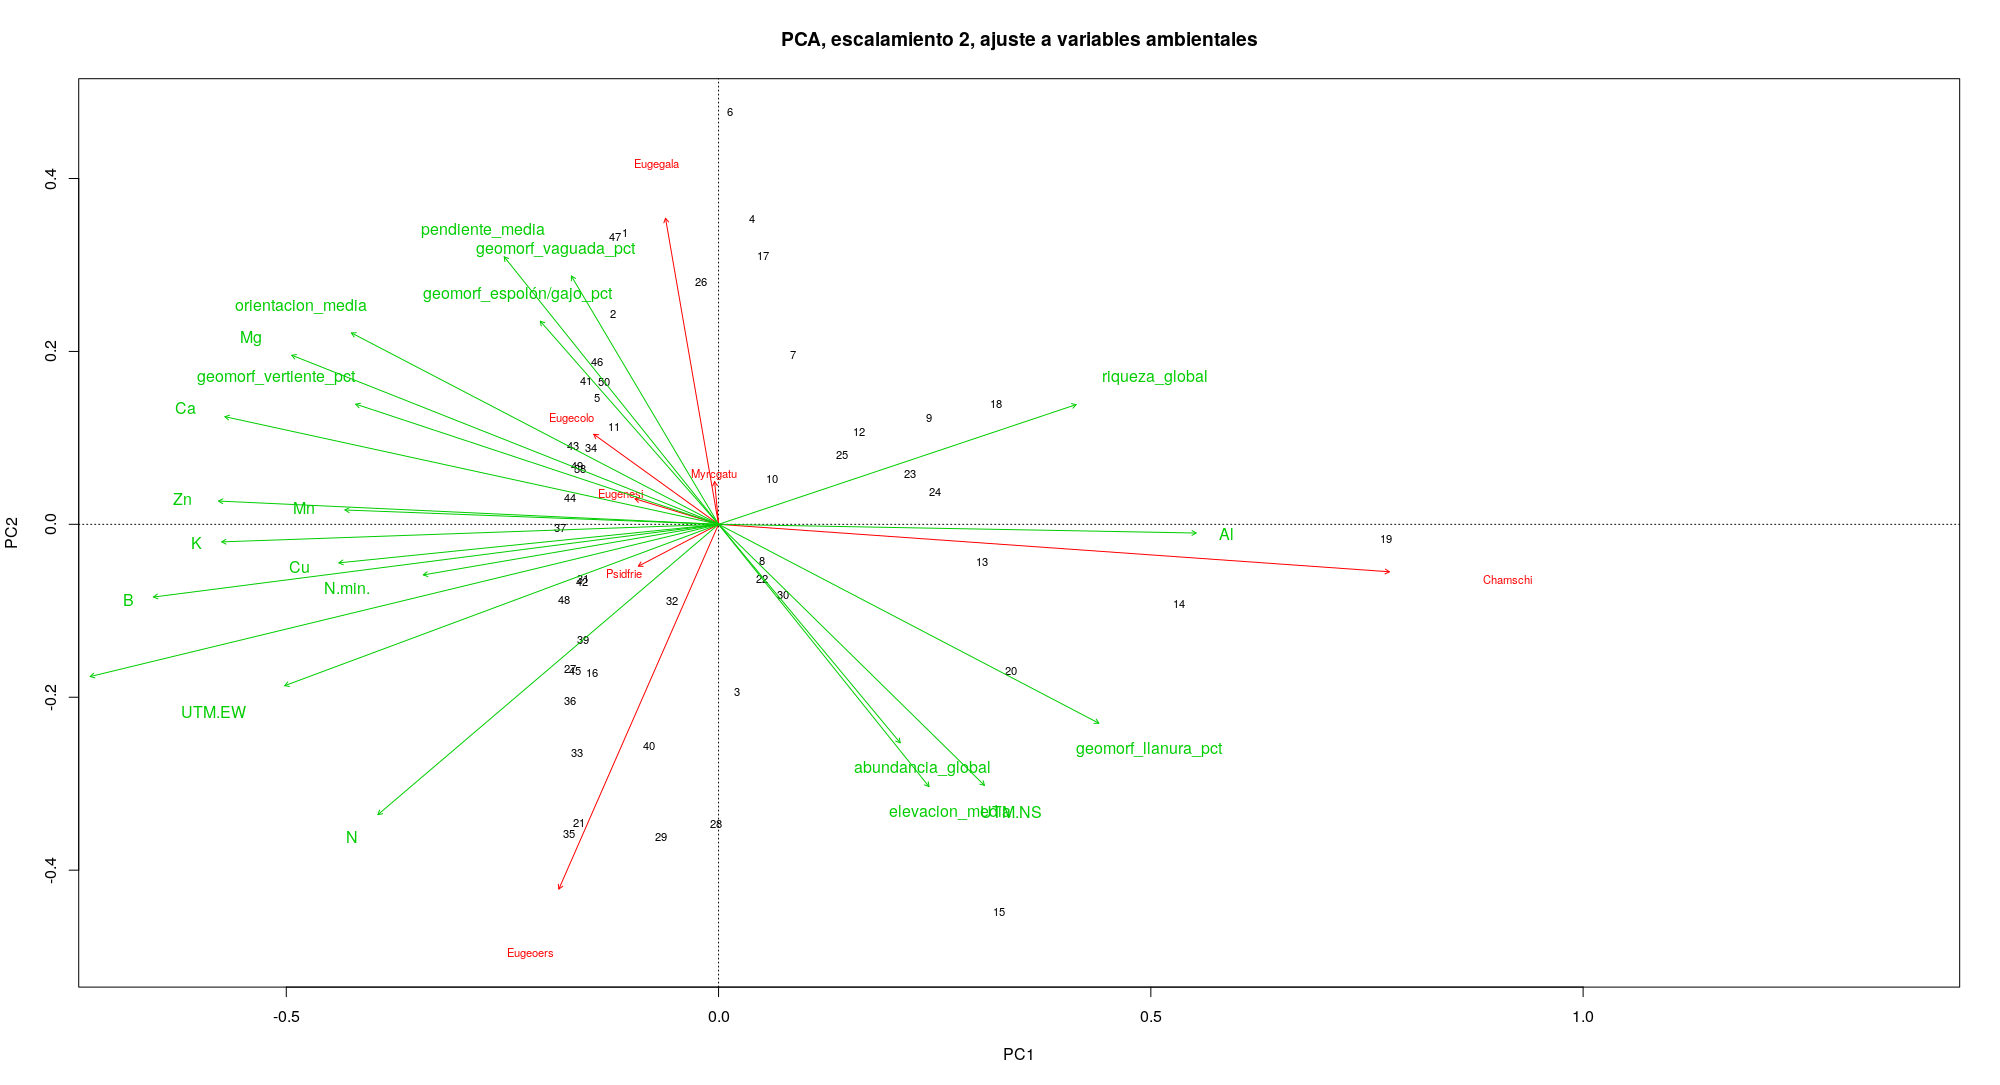
\includegraphics[width=0.50000\textwidth]{amb_spec_esc.png}
\caption{Distribución de especies asociadas a los sitios y a variables
ambientales (PCA).\label{fig:amb_esp_esc}}
\end{figure}

\begin{figure}
\centering
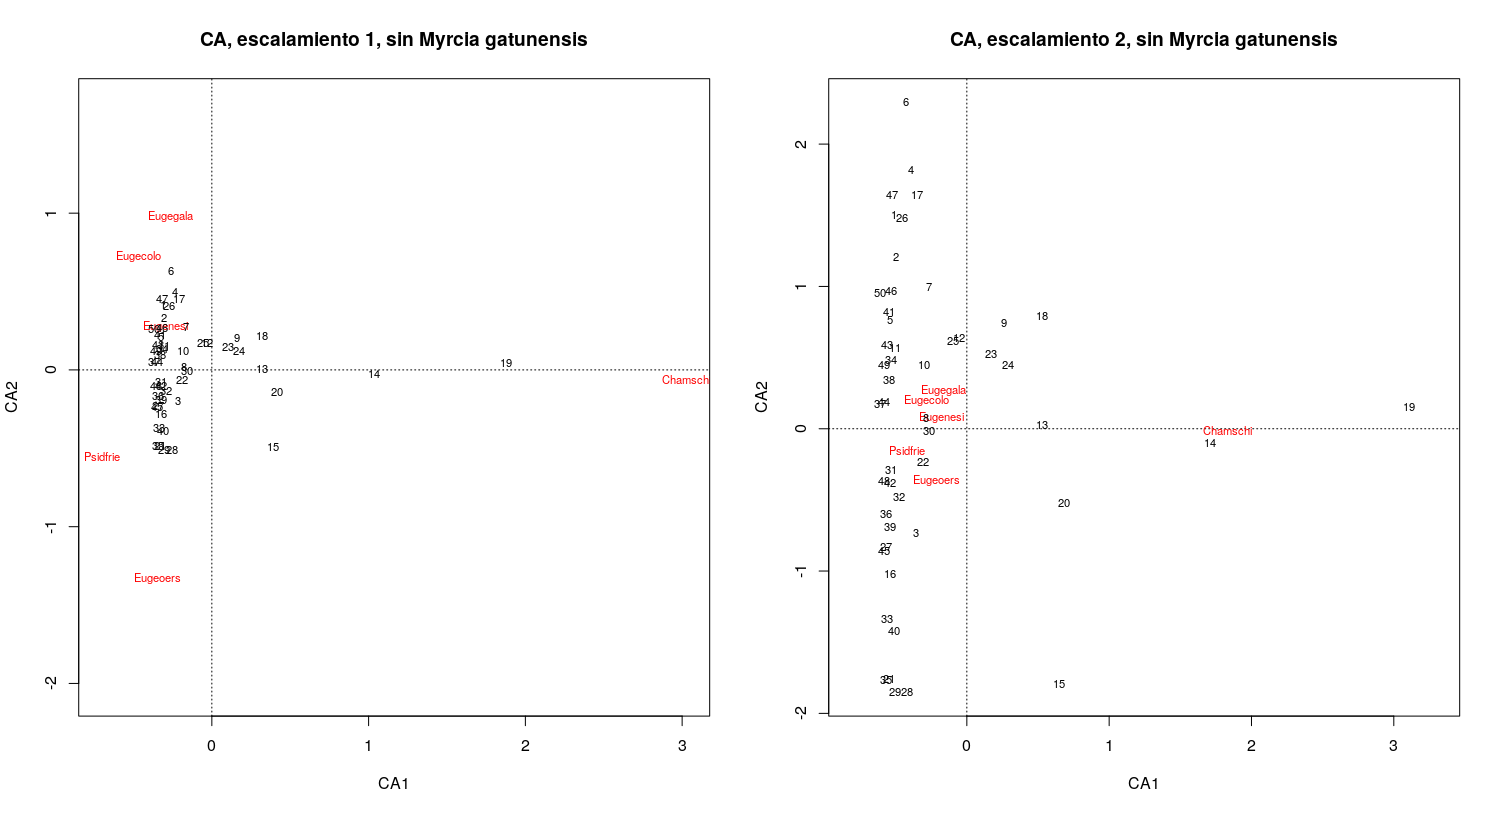
\includegraphics[width=0.50000\textwidth]{escalamiento sin myrcga.png}
\caption{Distribución de las espcies, excepto Mycia gatunensis, y de los
sitios (CA).\label{fig:escal_sin_myrcia}}
\end{figure}

\begin{longtable}[]{@{}cc@{}}
\caption{\label{tab:equivalencias} Equivalencias de los nombres de
especies de \emph{Myrtaceae}}\tabularnewline
\toprule
Nombre original & Equivalencias\tabularnewline
\midrule
\endfirsthead
\toprule
Nombre original & Equivalencias\tabularnewline
\midrule
\endhead
Eugenia galalonensis & Eugegala\tabularnewline
Eugenia oerstediana & Eugeoers\tabularnewline
Eugenia coloradoensis & Eugecolo\tabularnewline
Chamguava schippii & Chamschi\tabularnewline
Eugenia nesiotica & Eugenesi\tabularnewline
Psidium friedrichsthalianum & Psidfrie\tabularnewline
Myrcia gatunensis & Myrcgatu\tabularnewline
\bottomrule
\end{longtable}

\begin{figure}
\centering
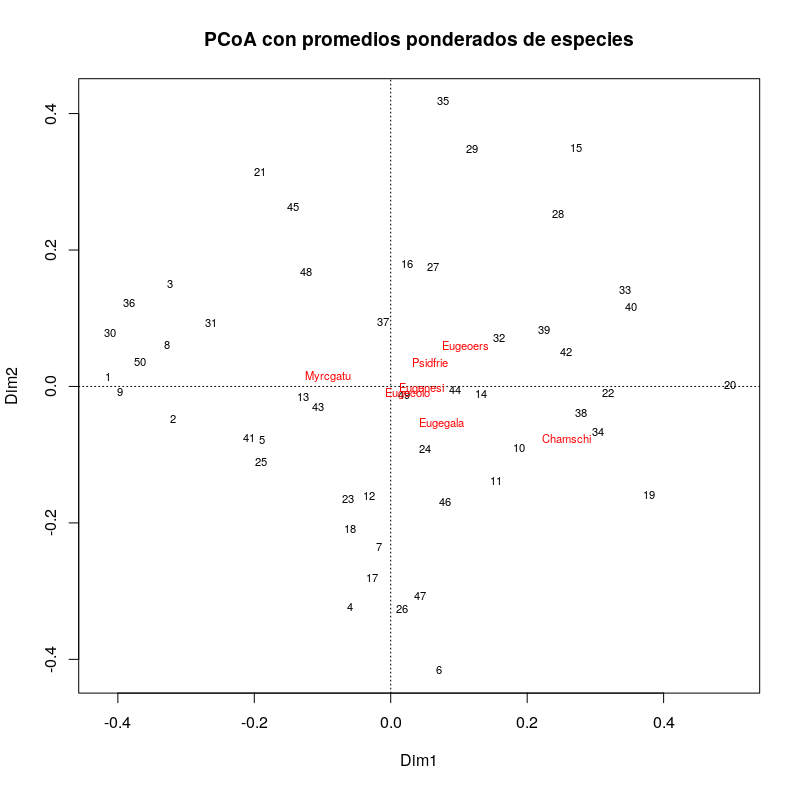
\includegraphics[width=0.90000\textwidth]{PCoA escalamiento_dat_mix.png}
\caption{Promedios ponderados de especies PCoA\label{fig:pcoa esc}}
\end{figure}

\begin{figure}
\centering
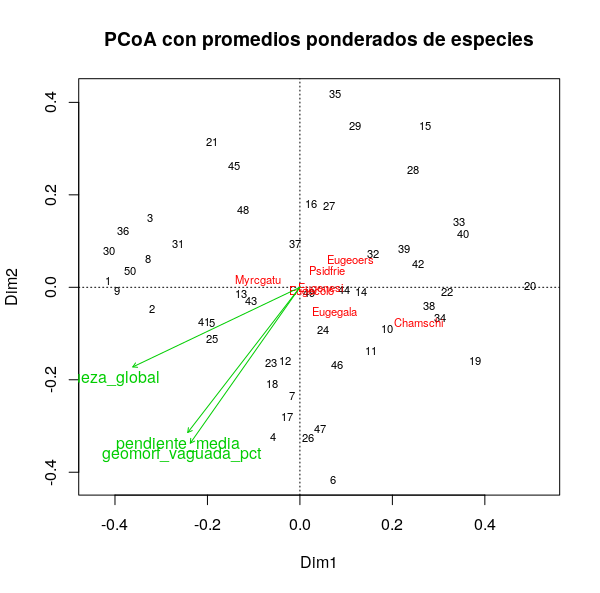
\includegraphics[width=0.90000\textwidth]{Pcoa_amb_spec_ escal.png}
\caption{Promedios ponderados de especies y variables ambientales
PCoA\label{fig:ambiental PCoA spec}}
\end{figure}

\begin{figure}
\centering
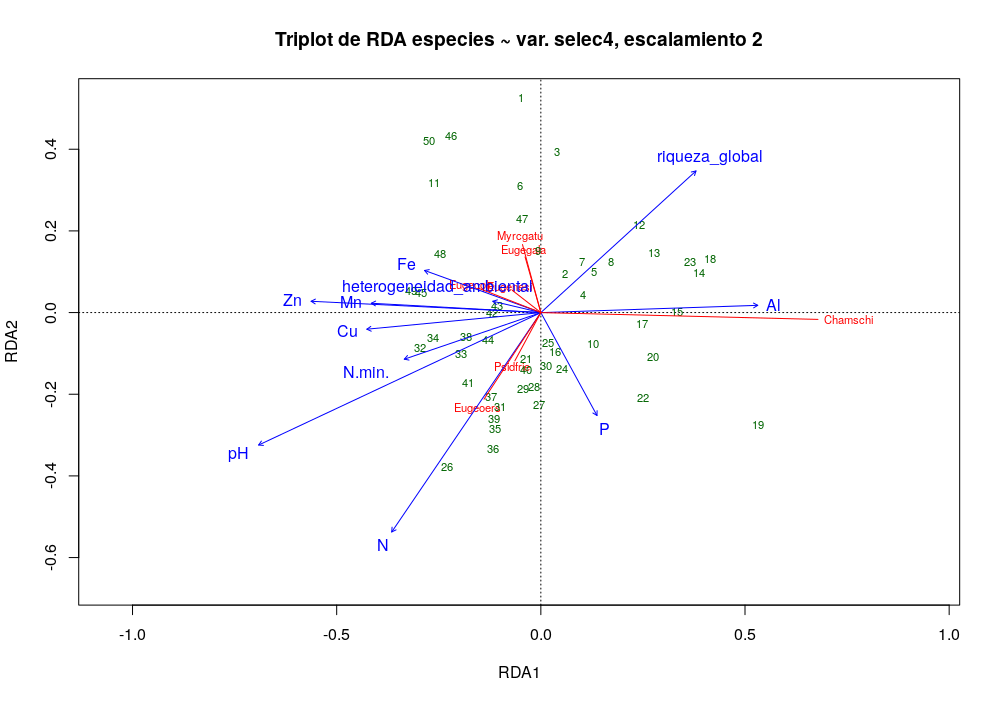
\includegraphics[width=0.90000\textwidth]{Rplorda_triplot_var.png}
\caption{Diagrama de especies, sitios y variables ambientales sin
colinealidad RDA.\label{fig:varesc2 tripo RDA}}
\end{figure}

\begin{figure}
\centering
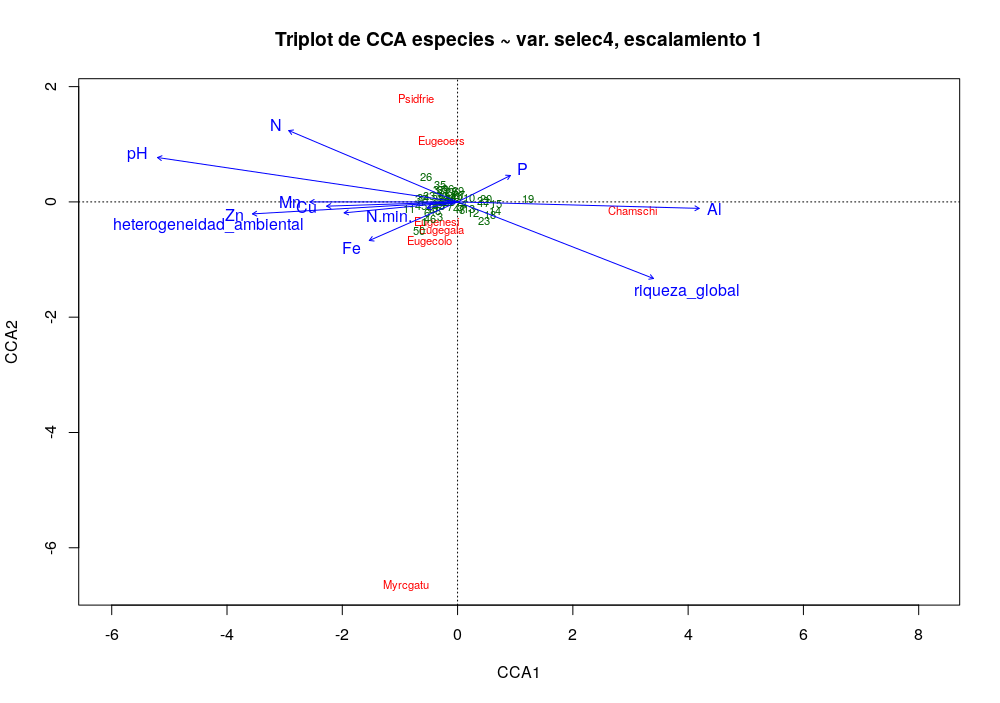
\includegraphics[width=0.90000\textwidth]{trip_cca_esca1.png}
\caption{Diagrama de especies, sitios y variables seleccionadas
CCA.\label{fig:esc1cca}}
\end{figure}

\begin{figure}
\centering
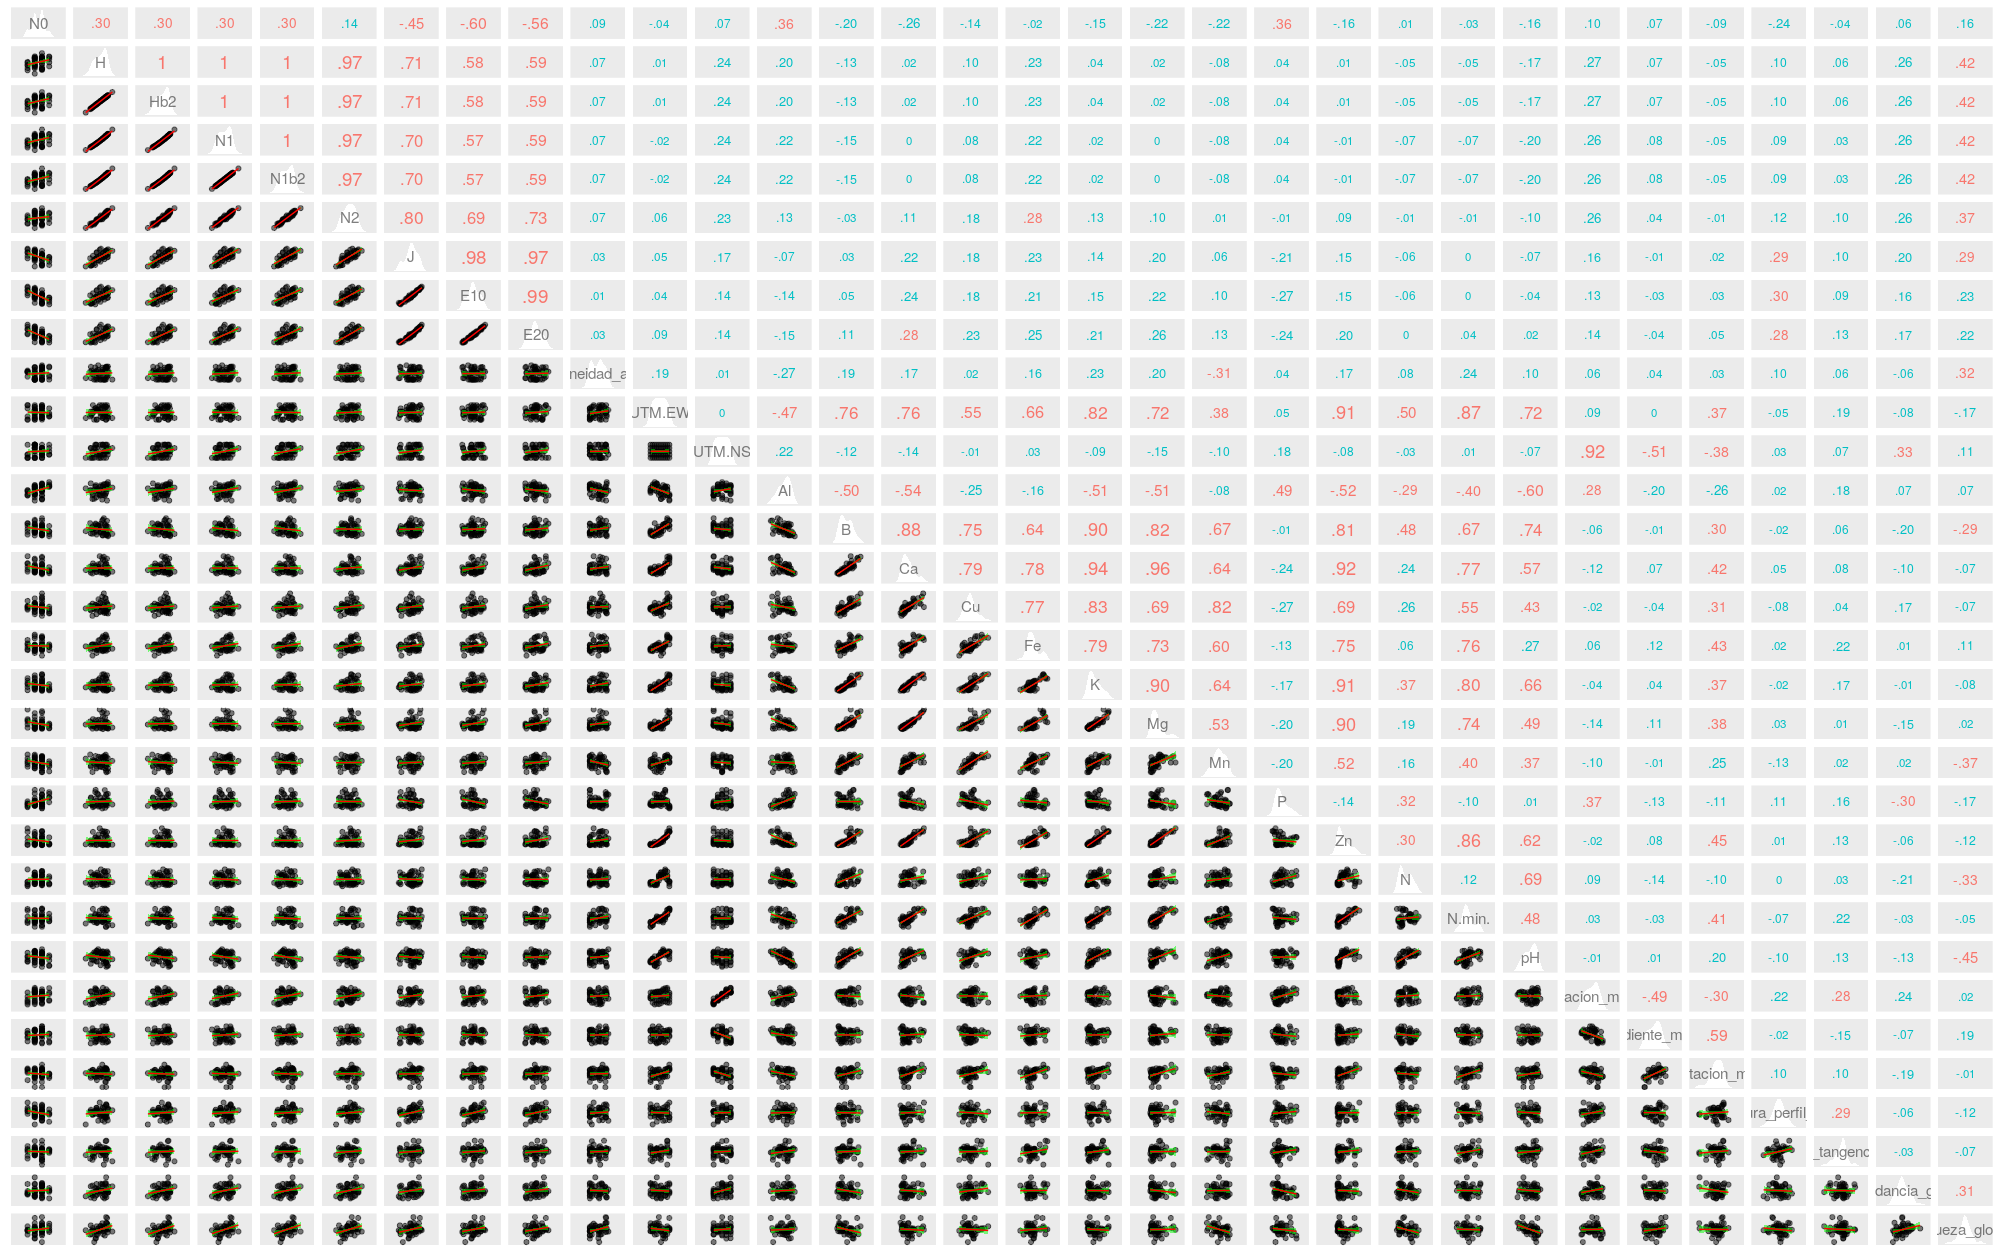
\includegraphics[width=1.00000\textwidth]{matriz_ind_var_amb.png}
\caption{Matriz de correlación entre índices de riqueza y algunas
variables
ambientales\label{fig:matriz de correlación de índices _con var amb}}
\end{figure}

\begin{figure}
\centering
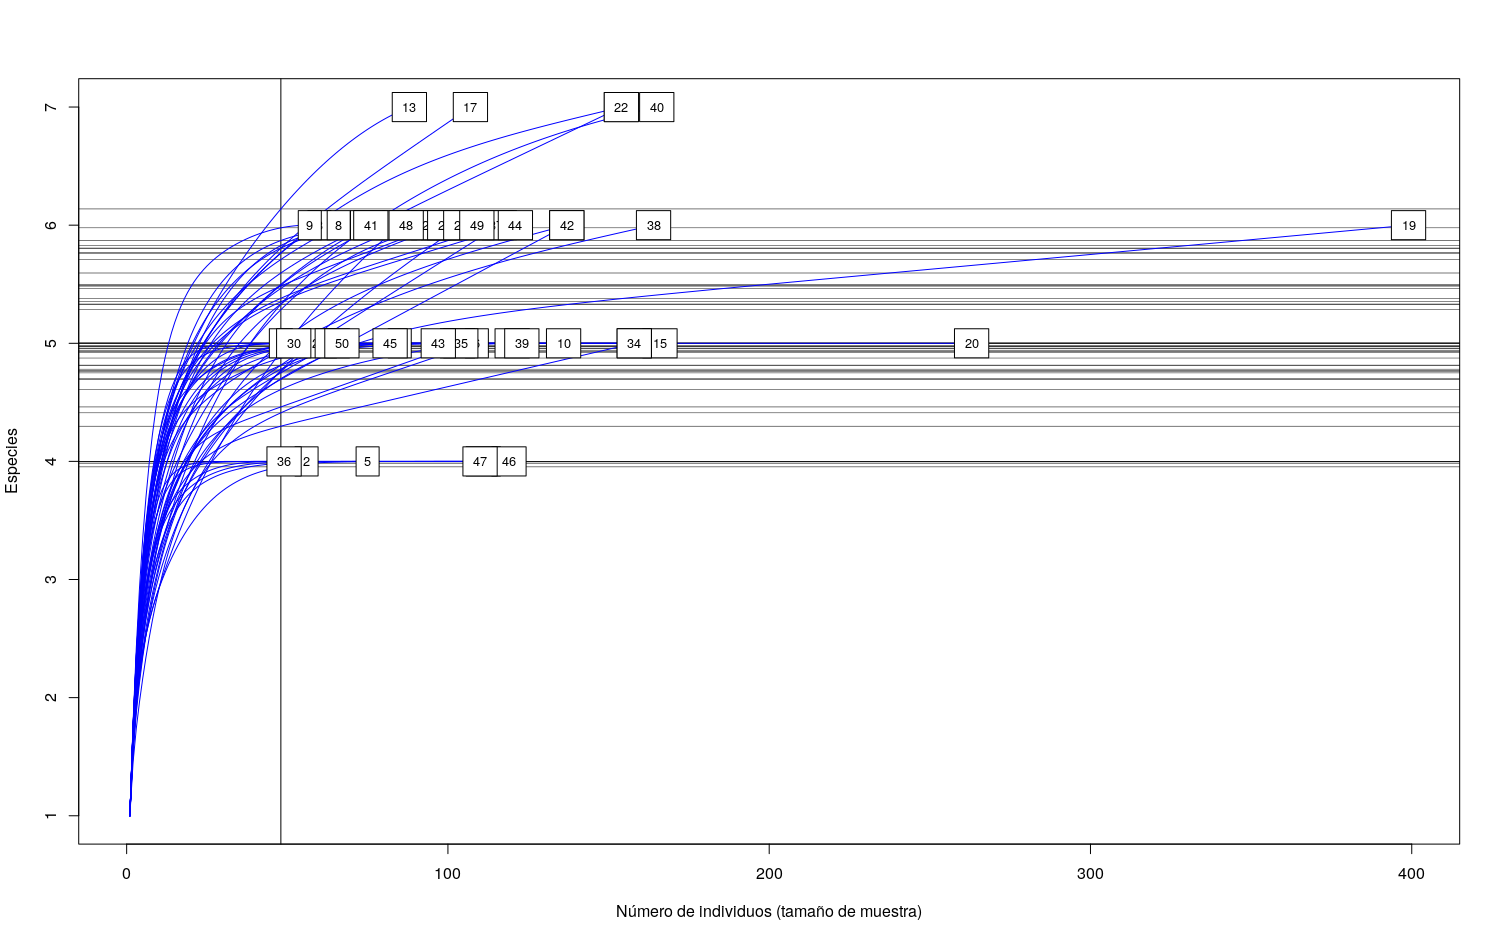
\includegraphics[width=1.00000\textwidth]{curva de rareza.png}
\caption{Curva de rareza de especies según sitios por
abundancia\label{fig:curva de rareza}}
\end{figure}

\begin{longtable}[]{@{}cc@{}}
\caption{\label{tab:estimadores} Estimadores de riqueza de
especies}\tabularnewline
\toprule
Estimadores de riqueza & Equivalencias\tabularnewline
\midrule
\endfirsthead
\toprule
Estimadores de riqueza & Equivalencias\tabularnewline
\midrule
\endhead
Total de especies & 7\tabularnewline
chao & 7\tabularnewline
chao.se & 0\tabularnewline
jack1 & 7\tabularnewline
jack1.se & 0\tabularnewline
jack2 & 7\tabularnewline
boot & 7\tabularnewline
boot.se & 5.161914e-08\tabularnewline
n & 50\tabularnewline
\bottomrule
\end{longtable}

\begin{figure}
\centering
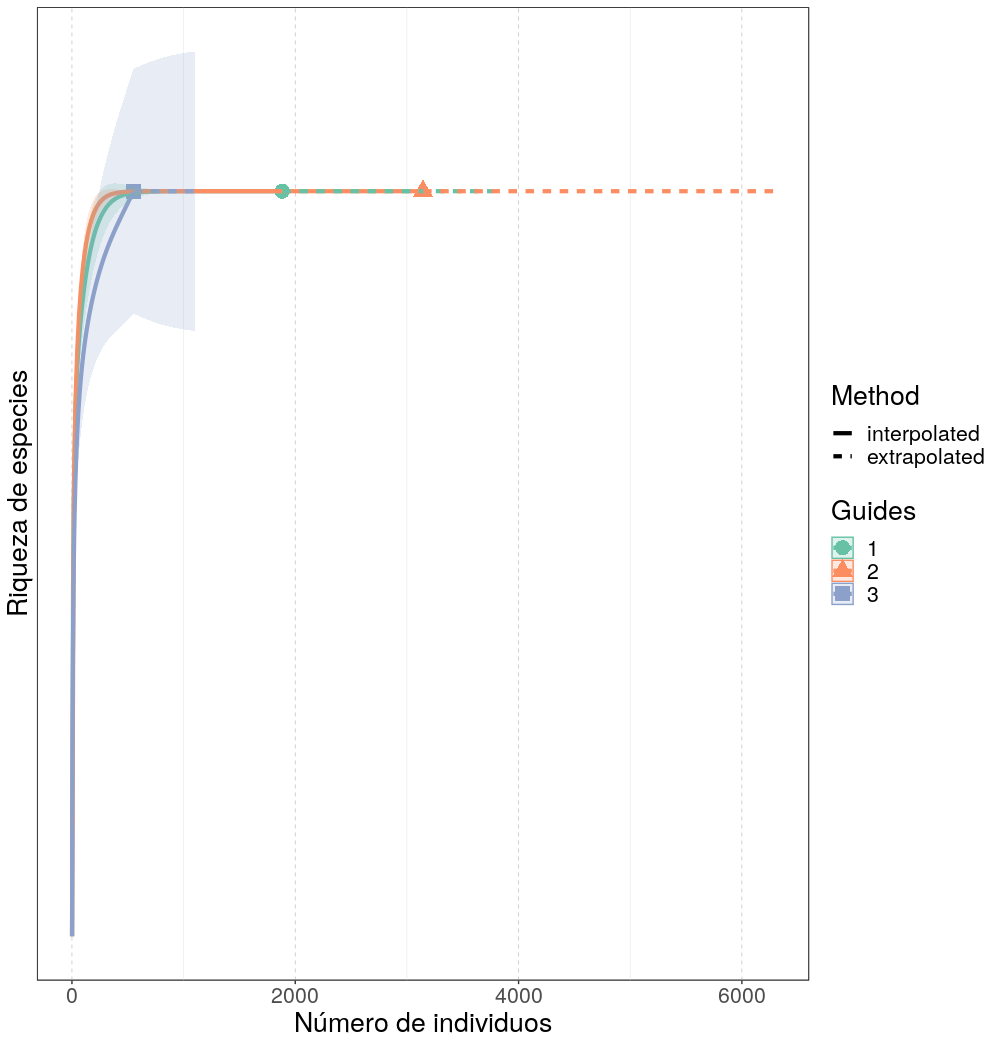
\includegraphics[width=0.90000\textwidth]{riq_espc_est.png}
\caption{Riqueza de especie estimada para los grupos obtenidos por el
método Ward\label{fig:riq_est}}
\end{figure}

\begin{figure}
\centering
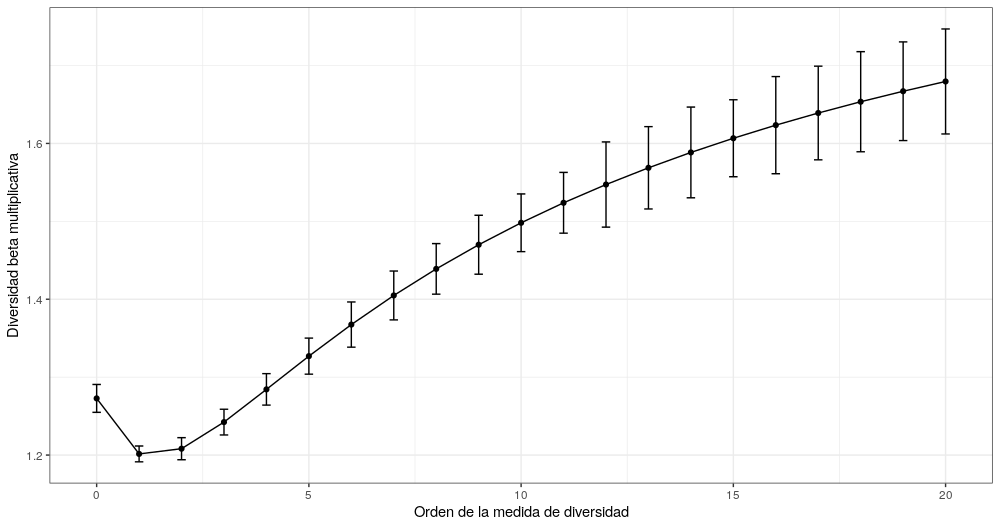
\includegraphics[width=0.90000\textwidth]{div_beta_multi.png}
\caption{Diversidad beta multiplicativa de la familia
\emph{Myrtaceae}\label{fig:beta}}
\end{figure}

\begin{figure}
\centering
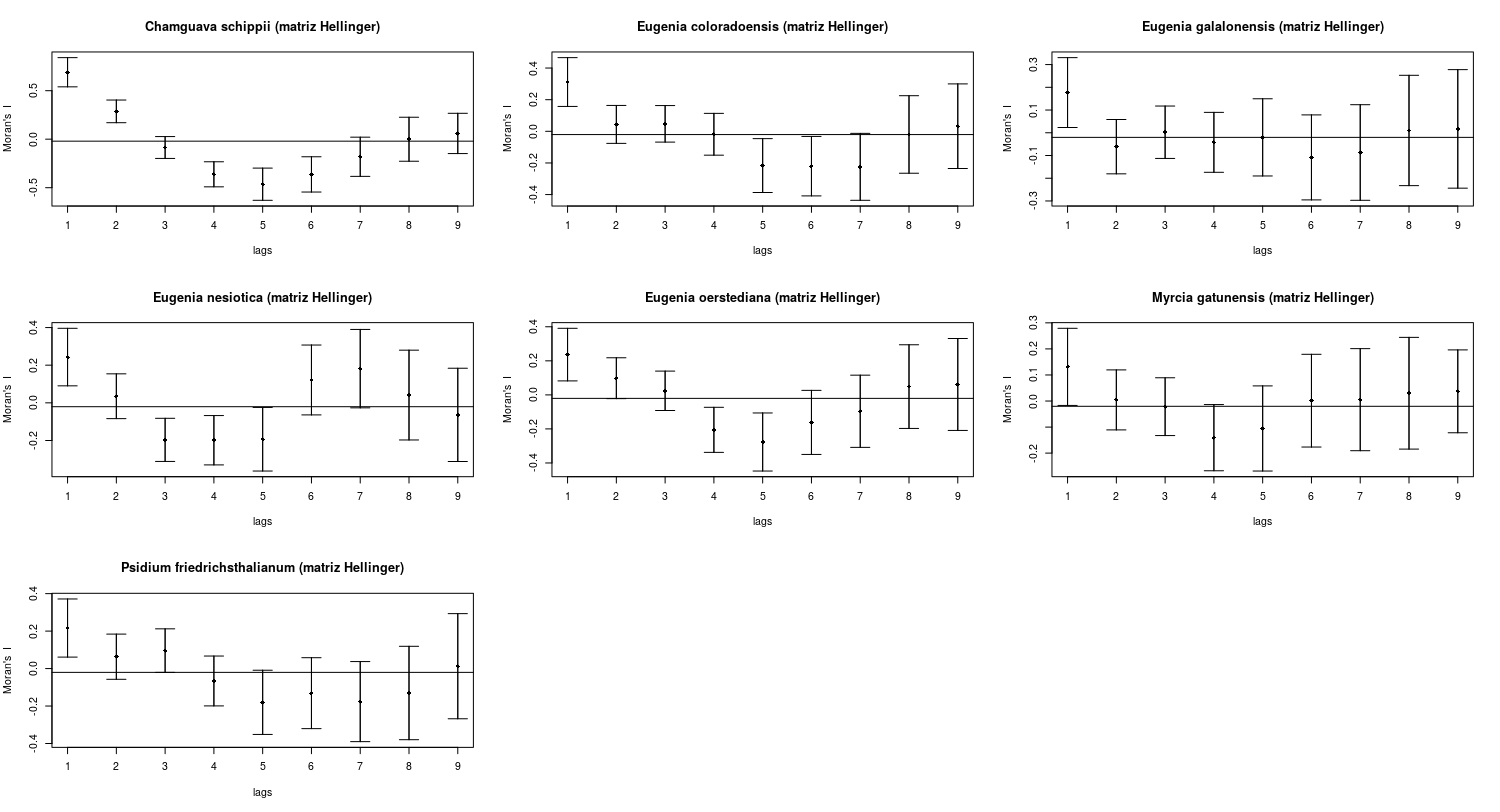
\includegraphics[width=0.90000\textwidth]{correl_abu_esp_sitios.png}
\caption{Correlograma de abundancia de especies por sitios
autocorrelacionados\label{fig:correlog_espc}}
\end{figure}

\begin{figure}
\centering
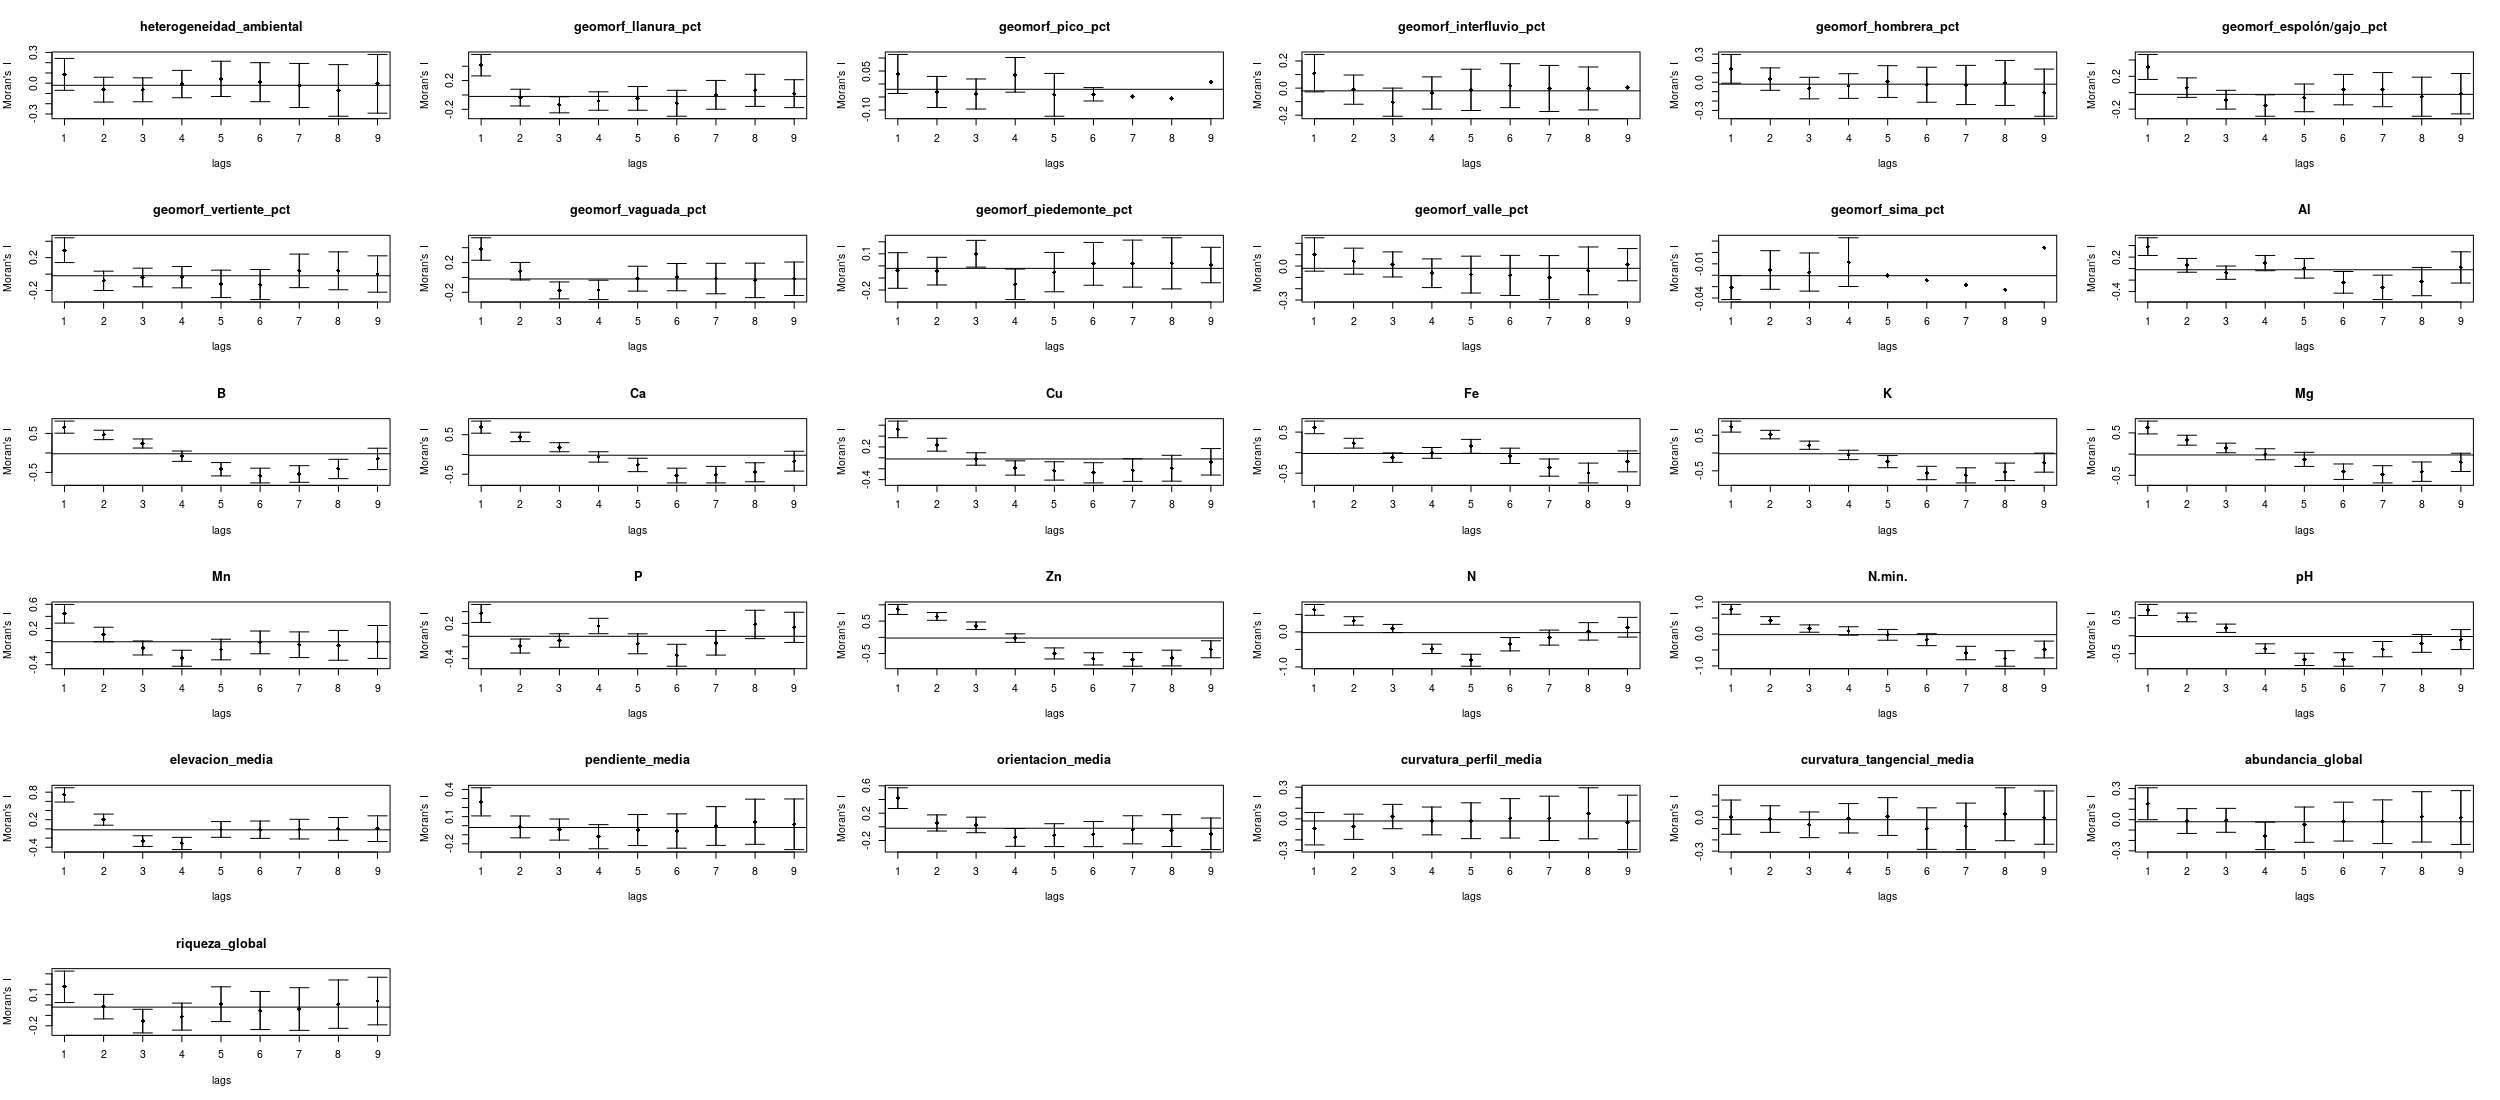
\includegraphics[width=1.00000\textwidth]{amb_corrl.png}
\caption{Correlograma de variables ambientales autocorrelacionadas por
sitios\label{fig:amb_correl}}
\end{figure}

\begin{figure}
\centering
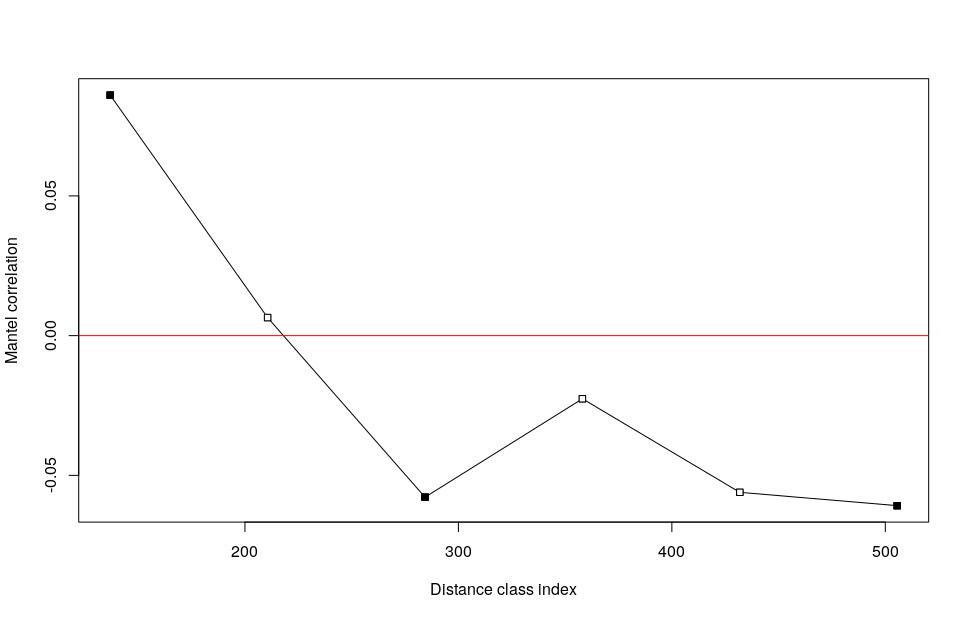
\includegraphics[width=0.90000\textwidth]{mantel_dist_corr.png}
\caption{Correlograma de dos matrices de comunidad autocorrelacionadas
usando matriz de distancia\label{fig:mantel_distancia}}
\end{figure}

\begin{figure}
\centering
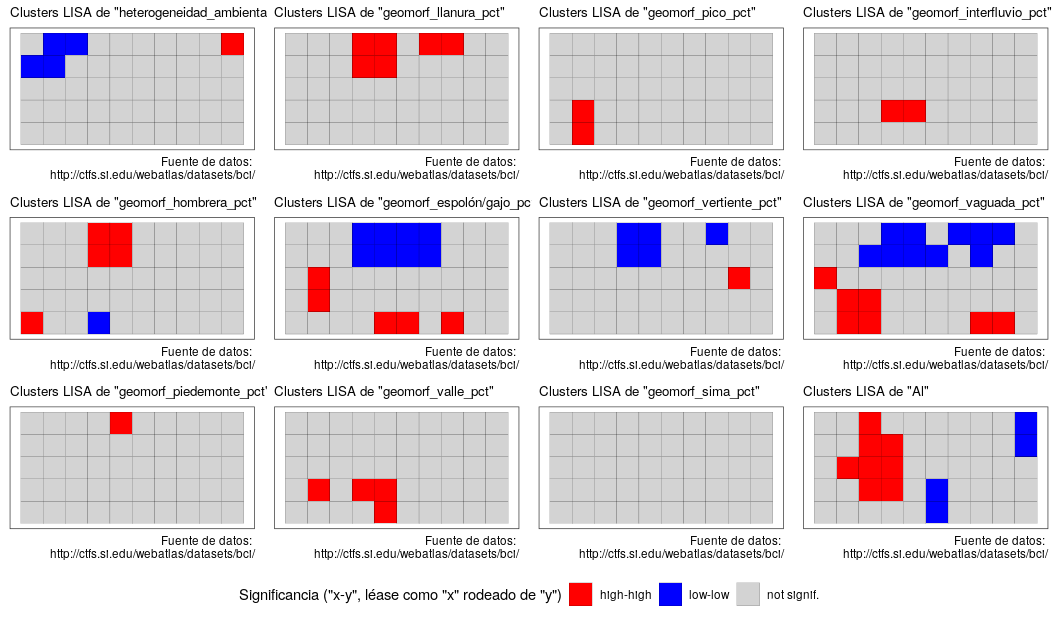
\includegraphics[width=0.90000\textwidth]{LISA_amb.png}
\caption{Modelos LISA Cluster de autocorrelación espacial de variables
ambientales, según las pruebas de permutación\label{fig:amb_perm}}
\end{figure}

\begin{figure}
\centering
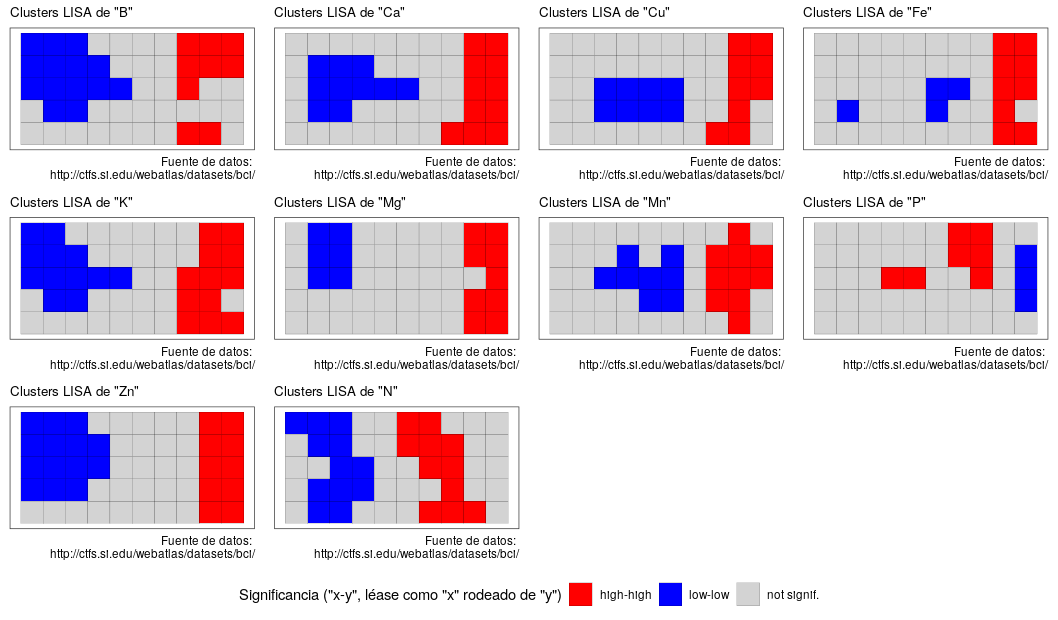
\includegraphics[width=0.90000\textwidth]{LISA_suelo.png}
\caption{Modelos LISA Cluster de autocorrelación espacial de variables
de suelo, según las pruebas de permutación\label{fig:perm_suelo}}
\end{figure}

\begin{figure}
\centering
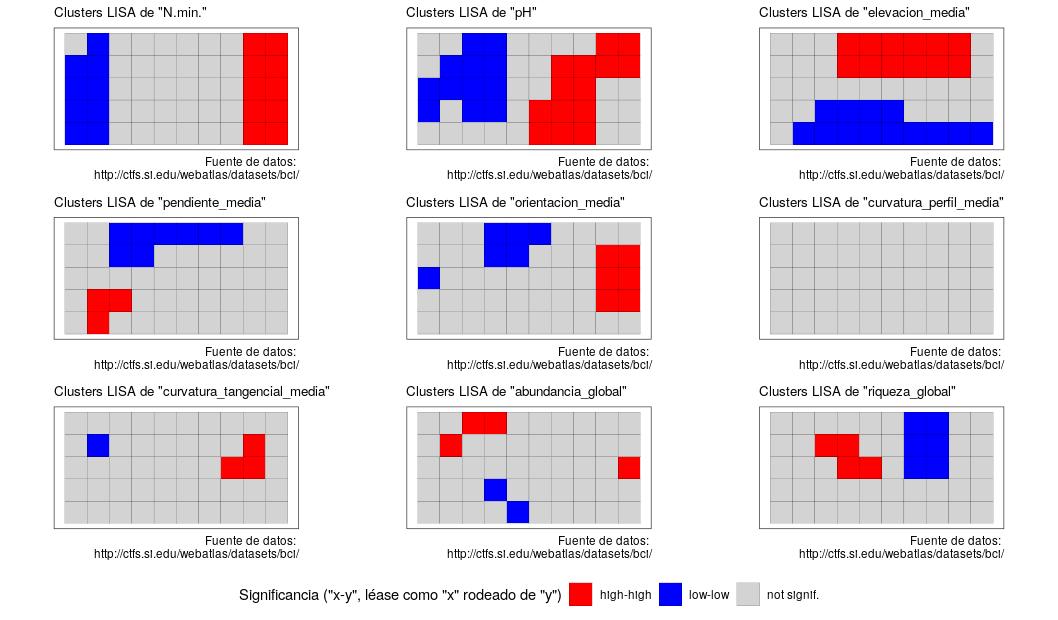
\includegraphics[width=0.90000\textwidth]{LISA_suelo2.png}
\caption{Modelos LISA Cluster de autocorrelación espacial de variables
ambientales, según las pruebas de permutación\label{fig:suelo2}}
\end{figure}

\begin{figure}
\centering
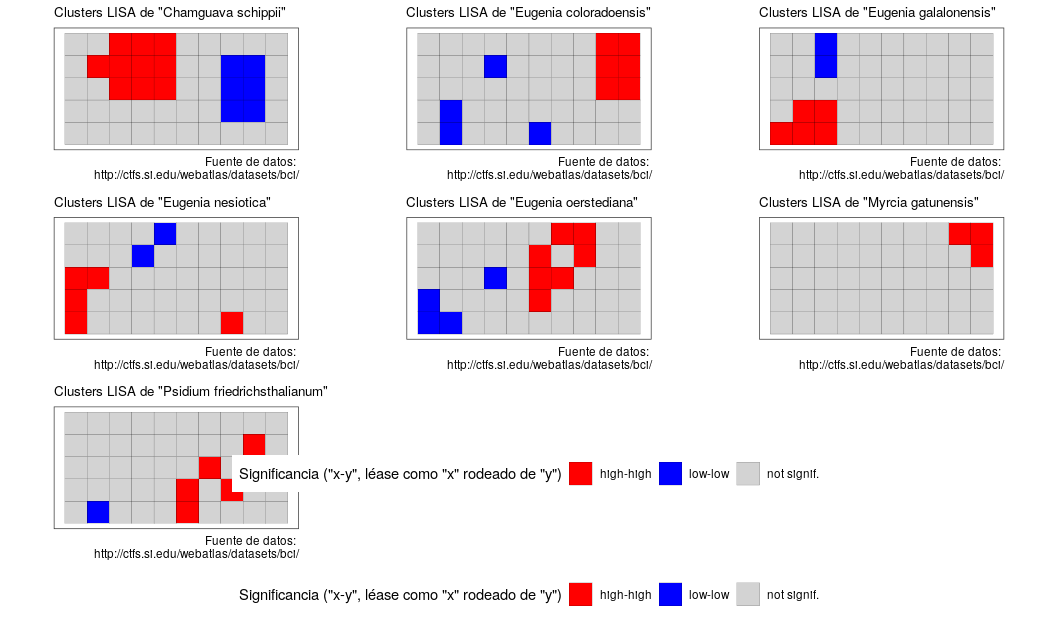
\includegraphics[width=0.90000\textwidth]{LISA_espc_trans.png}
\caption{Modelos LISA Cluster de autocorrelación espacial de las
especies transformadas, según las pruebas de
permutación\label{fig:espc_perm}}
\end{figure}

\begin{figure}
\centering
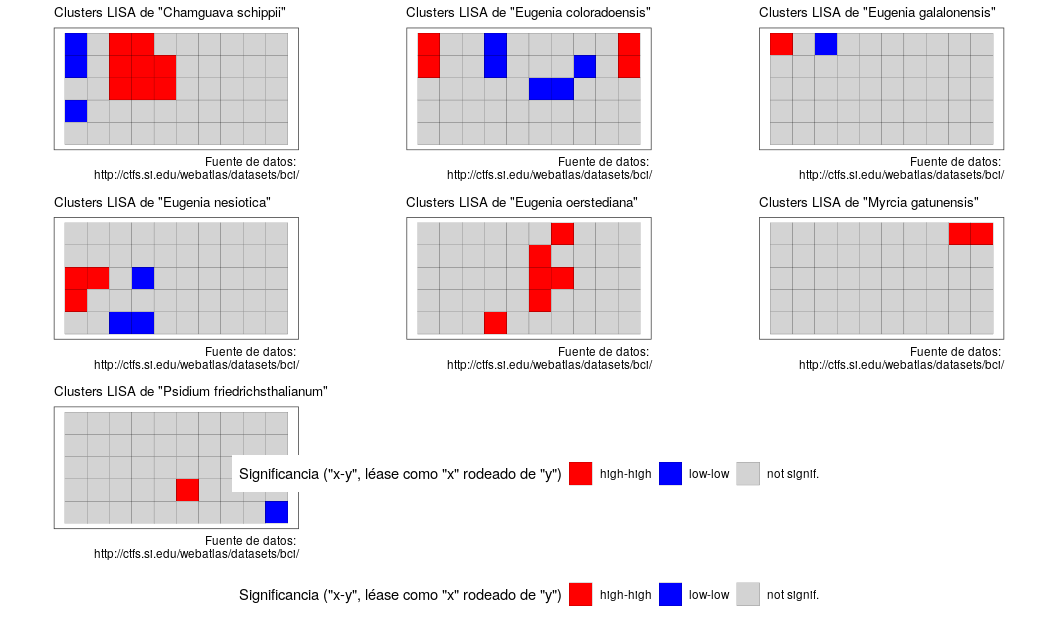
\includegraphics[width=0.90000\textwidth]{LISA_espc_sin_tend.png}
\caption{Modelos LISA Cluster de autocorrelación espacial de especies
transformadas sin tendencias, según las pruebas de
permutación\label{fig:sinten}}
\end{figure}

\section{\texorpdfstring{\emph{Script}
reproducible}{Script reproducible}}\label{script-reproducible}

\subsection{Análisis exploratorio de
datos.}\label{anuxe1lisis-exploratorio-de-datos.}

\begin{verbatim}
#' ---
#' title: "Análisis exploratorio de datos. Riqueza y abundancia"
#' author: "JR"
#' date: "13 de octubre, 2020"
#' output: github_document
#' ---

#' ### Área de cargar paquetes
library(vegan)
library(tidyverse)
library(sf)
source('biodata/funciones.R')

#' ### Área de cargar datos
#' Censo (el objeto se carga con prefijo "censo") y matriz de comunidad (prefijo "mc")
load('biodata/Myrtaceae.Rdata')
load('biodata/matriz_ambiental.Rdata') #Matriz ambiental, se carga como "bci_env_grid"

#' ### Imprimir datos en pantalla (impresiones parciales con head)
head(censo_myrtc)
head(mc_myrtc)
bci_env_grid # No necesita imprimirse parcialmente

#' ### También podemos usar
#' Requiere que se haya cargado ya la colección tidyverse
censo_myrtc %>% tibble
mc_myrtc %>% tibble

#' ### Lista de especies
sort(colnames(mc_myrtc))

#' ### Número de sitios, tanto en matriz de comunidad como en ambiental
#' Verifica que coinciden
nrow(mc_myrtc) #En la matriz de comunidad
nrow(bci_env_grid) #En la matriz ambiental

#' ### Riqueza numérica de especies (usando matriz de comunidad) por quadrat
#' Nota: cargar paquete vegan arriba, en el área de paquetes
specnumber(mc_myrtc)
sort(specnumber(mc_myrtc)) # Ordenados ascendentemente
summary(specnumber(mc_myrtc)) # Resumen estadístico

#' ### Abundancia de especies por quadrat
sort(rowSums(mc_myrtc))
summary(rowSums(mc_myrtc)) # Resumen estadístico

#' ### Abundancia por especie
sort(colSums(mc_myrtc))
summary(colSums(mc_myrtc)) # Resumen estadístico

#' ### Riqueza numérica de toda la "comunidad"
specnumber(colSums(mc_myrtc))

#' ### Abundancia de toda la comunidad
sum(colSums(mc_myrtc))

#' ### Una tabla para el manuscrito, es necesario asignarle nombre
#' Para esto, usaré la colección "tidyverse"
abun_sp <- censo_myrtc %>%
  group_by(Latin) %>% 
  count() %>% 
  arrange(desc(n))
abun_sp

#' ### Un gráfico para el manuscrito
#' Gráfico de mosaicos de la abundancia por especie por cuadros
abun_sp_q <- crear_grafico_mosaico_de_mc(mc_myrtc, tam_rotulo = 12)
abun_sp_q
\end{verbatim}

\begin{verbatim}
#' ---
#' title: "Análisis exploratorio de datos. Colección tidyverse"
#' author: "JR"
#' date: "18 de octubre, 2020"
#' output: github_document
#' ---

#' # ¿Qué es tidyverse?
#' 
#' Es una colección de paquetes con los que podrás importar, transformar, visualizar, modelar y presentar datos. La colección se compone de 8 paquetes, de los cuales verás sobre todo 3: `dplyr`, `tidyr` y `ggplot2`.
#' 
#' Todos estos paquetes comparten estructuras comunes. Una de las herramientas que incorpora la colección es la pipa `%>%` (**SHORTCUT: `CTRL+SHIFT+M`**), la cual importa desde el paquete `magrittr`. Usarás la pipa para construir "tuberías" de procesamiento sin necesidad de crear objetos intermedios. En una tubería, puedes interpretar la pipa como **"luego"**, y verás más adelante por qué. La función principal de la pipa (tiene muchas, pero esta es la más importante) es pasar el resultado del objeto a su izquierda como primer argumento de la función a su derecha. El siguiente ejemplo explica su uso:
#' 
#' `objeto1 %>% funcion1()` es equivalente a `funcion1(argumento1 = objeto1)`
#' 
#' > La idea del *pipe* pertenece a la tradición de sistemas tipo Unix y, en origen, su función era comunicar distintos procesos, usando la salida estándar de uno (*stdout*) como entrada estándar (*stdin*) del siguiente.
#' 
#' Su ventaja radica en que, si necesitaras continuar procesando los datos, no tendrás que anidar ni crear objetos intermedios. En el siguiente ejemplo, asigno el resultado de una cadena al objeto nombrado `resultado`:
#' 
#' `resultado <- objeto1 %>% funcion1() %>% funcion2() %>% funcion3()`
#' 
#' Puedes leer lo anterior como *"objeto1 pasa como primer argumento de funcion1, **luego** el resultado de funcion1 pasa como primer argumento de funcion2, **luego** el resultado de funcion2 pasa como primer argumento de funcion3*.
#' 
#' Para replicar esta operación sin la pipa, podrías realizarlo de, por ejemplo, dos maneras distintas:
#' 
#' * Opción 1, anidar:
#' 
#' `resultado <- funcion3(funcion2(funcion1(objeto1)))`
#' 
#' Opción 2, crear objetos intermedios:
#' 
#' `tmp1 <- funcion1(objeto1)`
#' `tmp2 <- funcion2(tmp1)`
#' `resultado <- funcion3(tmp2)`
#' 
#' Notarás que, comparada con estas dos últimas opciones, la tubería es más limpia que estas dos últimas opciones. La tubería puedes leerla de forma encandenada, a diferencia del estilo anidado y de creación de objetos intermedios, que añade una cierta complejidad de lectura para el usuario/a, sobre todo para personas sin conocimientos de programación. Precisamente por esta razón fue que decidí introducir la colección tidyverse, para así mostrarte algunas ideas que podrás aplicar a tus datos y, en principio, para facilitarte la vida ("*no me ayude' tali*"). Ahora bien, si decides programar en R más adelante, deberás aprender las capacidades de programación orientada a objetos y programación funcional de R.
#' 
#' ¡Comencemos!
#' 
#' ## Paquetes
#' 
library(tidyverse)
library(sf)
#' 
#' > `sf` te ayudará a leer el objeto `bci_env_grid` como un *simple feature*, el cual se encuentra dentro del archivo `biodata/matriz_ambiental.Rdata`. Esto extenderá las capacidades espaciales del objeto.
#' 
#' ## Cargar datos
#' 
load('biodata/matriz_ambiental.Rdata')
load('biodata/Myrtaceae.Rdata')
#'  
#' ## Paquete `dplyr`
#' 
#' Te servirá para manipular datos mediante verbos. Los verbos de `dplyr` que conocerás son (hay muchos otros): `select()`, `filter()`, `arrange()`, `mutate()`, `group_by()`, `summarise()` y `join`.
#' 
#' ### Verbo `select`
#' 
#' Comúnmente, necesitas seleccionar una o varias columnas de una tabla. Para esto existe el verbo `select`. Te muestro un ejemplo aplicado a la matriz de comunidad (que por ahora la verás como `simple feature`), seleccionando las columnas `id` (número identificador de quadrat) y `pH` (pH del suelo):
bci_env_grid %>%
  select(id, pH)
#' > Importante: el objeto `bci_env_grid` permanece intacto, a menos que se use dicho nombre para reasignarlo a otro objeto. Mientras no se use el asignador `<-`, sólo verás que manipulo y visualizo copias del objeto original.
#' Fíjate en la clase del objeto `bci_env_grid`. Para ello usaré la función de R `class`. No sólo se admiten verbos `dplyr`, cualquier función puede usarse:
bci_env_grid %>%
  class
#' El objeto `bci_env_grid` es a la vez de clase `sf` (*simple feature*) y `data.frame`, es decir, es tanto tabla como objeto espacial, por lo que se puede representar en un mapa. Este objeto no pierde la clase `sf`, por lo que verás que aparece información geométrica y geoespacial en el encabezado, y luego un extracto de la tabla de datos (como máximo, las 10 primeras filas). Para convertirlo a un simple `data.frame`, hay que "tumbar" su geometría con `st_drop_geometry`:
bci_env_grid %>%
  select(id, pH) %>%
  st_drop_geometry
#' Fíjate ahora en la clase de `bci_env_grid %>% select(id, pH) %>% st_drop_geometry`, que en este caso es sólo `data.frame`:
bci_env_grid %>%
  select(id, pH) %>%
  st_drop_geometry %>%
  class
#' > Al introducir un `<enter>` después de la pipa, el código puede continuar en la línea siguiente. Esto se hace para evitar que la línea de código sea legible sin necesidad de desplazarse hacia la derecha (es aconsejable no superar los 80 caracteres en una misma línea de código, según recomiendan en la [Google’s R Style Guide](https://google.github.io/styleguide/Rguide.html)). Como convención, escribiré un `<enter>` después de cada operador pipa.
#' 
#' Seleccionaré, y a la vez renombraré, dos columnas con `select` (recuerda: no estoy modificando el objeto original, simplemente trabajo en copias no asignadas). De paso, sólo mostraré las 6 primeras filas al aplicar `head` al final de la tubería (no sólo se admiten verbos `dplyr`, cualquier función de R puede entrar en la tubería):
bci_env_grid %>%
  select(id_de_quadrat = id, pH_del_suelo = pH) %>%
  st_drop_geometry %>%
  head
#' 
#' Otra funcionalidad de `select` es poder seleccionar columnas según patrones. Por ejemplo, si quisera seleccionar únicamente las variables sobre geomorfología (todas las columnas que comienzan por `geomorf`), podría hacerlo con relativa facilidad usando la función de ayuda `contains`
#' 
bci_env_grid %>%
  select(contains('geomorf')) %>%
  st_drop_geometry
#' ...y también usando expresiones regulares con `matches`, usando por ejemplo dos cadenas de caracteres...
bci_env_grid %>%
  select(matches('geomorf|habit', ignore.case = F)) %>%
  st_drop_geometry
#' ...o pidiendo todas las columnas que comienzan por mayúsculas, excepto las que comienzan por "U", lo cual excluye las coordenadas (e.g. `UTM.NS`), y deja sólo los elementos de análisis de suelo.
bci_env_grid %>%
  select(matches('^[A-T,Z]', ignore.case = F)) %>%
  st_drop_geometry
#' ### Verbo `filter`
#' 
#' Ahora mostraré sólo los elementos con `pH` mayor que 5, usando el verbo `filter`
bci_env_grid %>%
  select(id, pH) %>%
  st_drop_geometry %>%
  filter(pH>5)
#' O filtro por aquellos con `id` 31 y 50:
bci_env_grid %>%
  select(id, pH) %>%
  st_drop_geometry %>%
  filter(id == c(31, 50))
#' 
#' ### Verbo `arrange`
#' 
#' Pruebo también con la matriz de comunidad. Por ejemplo, introduzco en la tubería la función `colSums`, que devuelve un vector cuyos elementos están nombrados (tienen un atributo, en este caso, el nombre de especie), donde cada elemento representa la abundancia por especie.
mc_myrtc %>%
  colSums
#' Y también obtengo la abundancia por quadrat.
mc_myrtc %>%
  rowSums
#' Uso a continuación el verbo `arrange` para mostrar los registros de la matriz ambiental ordenados ascendentemente por pH.
bci_env_grid %>%
  select(id, pH) %>%
  st_drop_geometry %>%
  arrange(pH)
#' Ahora usaré `arrange` para mostrar los registros de la matriz ambiental ordenados DESCendentemente por pH.
bci_env_grid %>%
  select(id, pH) %>%
  st_drop_geometry %>%
  arrange(desc(pH))
#' 
#' ### Verbo `mutate`
#' 
#' Usaré el verbo `mutate` para crear una nueva columna. Por ejemplo, creo una columna que contenga `habitat` y `quebrada` separadas por una coma:
bci_env_grid %>%
  st_drop_geometry %>%
  select(habitat, quebrada) %>% 
  mutate(habitat_quebrada = paste(habitat, quebrada, sep = ', '))
#' Ahora `mutate`, pero con números: creo una columna de área de cada cuadro (necesitas también la función `st_area`, del paquete `sf`):
bci_env_grid %>%
  mutate(area = st_area(geometry)) %>%
  select(id, area) %>%
  st_drop_geometry %>%
  head
#' ...y ahora más complejo: obtengo la densidad de individuos por metro cuadrado, ordenados descendentemente por dicha densidad, y conservando sólo los 6 registros con mayores densidades.
bci_env_grid %>%
  mutate(area = st_area(geometry), densidad_indiv = abundancia_global/area) %>% 
  select(id, densidad_indiv) %>% 
  st_drop_geometry %>% 
  arrange(desc(densidad_indiv)) %>% 
  head
#' 
#' ### Verbos `group_by` y `summarise`
#' 
#' Los verbos `group_by` y `summarise` son útiles para producir resúmenes por grupos.
#' 
#' Agruparé la matriz ambiental por la columna `habitat`, dejando sólo las variables numericas que hagan sentido (por ejemplo, excluyo `id`, `UTM.EW`, `UTM.NS`), y lo asignaré a `agrupado_por_habitat` para luego reutilizarlo:
agrupado_por_habitat <- bci_env_grid %>%
  st_drop_geometry %>%
  group_by(habitat) %>% 
  select_if(is.numeric) %>%
  select(-id, -UTM.EW, -UTM.NS)
agrupado_por_habitat
#' Observa el encabezado: el objeto es `A tibble: 50 x 32` y hay 5 grupos (`Groups:   habitat [5]`). Calculo cuántos elementos (filas) hay por grupo:
agrupado_por_habitat %>% summarise(n = n())
#' ...y también algunos estadísticos de las columnas `pH`, `abundancia_global` y `riqueza_global` por ejemplo:
agrupado_por_habitat %>%
  summarise(
    n = n(),
    media_pH = mean(pH),
    media_abundancia = mean(abundancia_global),
    media_riqueza = mean(riqueza_global)
  )
#' ...o la media de todas las variables numéricas
agrupado_por_habitat %>%
  summarise_all(mean)
#' ...no caben, mejor por partes
agrupado_por_habitat %>%
  summarise_all(mean) %>% 
  select(1:6) %>% 
  print(width=300)
agrupado_por_habitat %>%
  summarise_all(mean) %>% 
  select(1,7:12) %>% 
  print(width=300)
agrupado_por_habitat %>%
  summarise_all(mean) %>% 
  select(1, 13:25) %>% 
  print(width=300)
agrupado_por_habitat %>%
  summarise_all(mean) %>% 
  select(1, 26:32) %>%
  print(width=300)
#' ...y no sólo un estadístico, sino varios:
agrupado_por_habitat %>%
  summarise_all(
    list(
      media = mean,
      mediana = median,
      varianza = var,
      minimo = min,
      maximo = max
    )
  )
#' Ejecuto también un ANOVA de una vía, de la `riqueza_global` respecto de `habitat` de tipo `Old*` (e.g. `OldHigh`, `OldLow`, `OldSlope`)
agrupado_por_habitat %>%
  filter(str_detect(habitat, 'Old*')) %>%
  oneway.test(formula = riqueza_global ~ habitat)
#' El resultado sugiere que "existen 'diferencias significativas' de `riqueza_global` entre `habitat` de tipo `Old*`". Esta expresión, "diferencias significativas", resuena mucho en ciencia hoy en día, y más bien "chirría". De ella hablaré más adelante, por lo pronto, donde quiera que la veas, levanta una ceja.
#' 
#' Finalmente, te muestro `join`. Más que una función, `join` es una función genérica con varios métodos para unir tablas que comparten al menos un atributo en común, siendo `inner_join` el más usado. Imagina un caso de uso: calculas abundancia de tu familia de plantas por cada quadrat de 1 ha. Ahora necesitas unir dicha información a la matriz ambiental. Aunque hay múltiples soluciones, `inner_join` es la que con mayor consistencia resuelve este problema.
#' 
#' Obtendré una tabla con dos columnas: código identificador de quadrat de 1 ha (le llamaré `id`), y abundancia de todas las plantas de mi familia por quadrat (le llamaré `abundancia_mi_familia`)
id_abundancia_fam <- mc_myrtc %>%
  mutate(abundancia_mi_familia = rowSums(.)) %>% 
  rownames_to_column(var = 'id') %>%
  mutate(id = as.numeric(id)) %>% #Numérico, garantiza compatibilidad con id de bci_env_grid
  select(id, abundancia_mi_familia)
id_abundancia_fam %>% tibble
#' Dado que `id_abundancia_fam` y `bci_env_grid` comparten el campo `id`, a través de éste se puede realizar la unión. Primero escribiré `bci_env_grid`, luego la función `inner_join`, que tiene como argumentos la tabla `x` y la tabla `y`. La tabla `x`, primer argumento, será `bci_env_grid`, y la tabla `y` será `id_abundancia_fam`. El campo de unión será `id`, el cual es compartido.
bci_env_grid %>%
  inner_join(y = id_abundancia_fam, by = 'id')
#' El resultado muestra la `bci_env_grid`, ahora con los datos de mi familia como parte de la matriz. Nótese que no asigné el objeto, por lo que la matriz ambiental original sigue intacta.
#' 
#' ## `tidyr`
#' 
#' Te ayudará a reordenar datos, mediante transformación de su estructura, para organizarlos de forma "tidy". Los verbos de `tidyr` que conocerás son (también cuenta con muchas otras): `pivot_longer()` (antiguamente `gather()`) y `pivot_wider()` (antiguamente `spread()`).
#' 
#' ### Verbo `pivot_longer`
#' 
#' Cuando necesitas reunir varias columnas, o lo que es lo mismo, hacerlas que pivoten a lo largo en la tabla, utilizas este verbo. Pasas de tener una tabla organizada a lo ancho a tenerla organizada a lo largo.
#' 
#' ![](https://uc-r.github.io/public/images/dataWrangling/gather1.png)
#' *Tomado de: UC Business Analytics R Programming Guide. Reshaping Your Data with tidyr. https://uc-r.github.io/tidyr*
#' 
#' Es común realizar "reunión" columnas cuando nos interesa aplicar análisis masivos a múltiples variables utilizando un criterio de agrupamiento. 
#' 
#' Pongo un ejemplo. Por tipo de hábitat, ¿cuánto es el promedio de los porcentajes de cada uno de los 10 tipos de unidades geomorfológicas? `pivot_longer` lo hará al final, pero primero, hay que seleccionar solo las columnas de porcentajes de unidades geomorfológicas y la de habitat...
pivotpaso1 <- bci_env_grid %>%
  st_drop_geometry %>% 
  select(matches('geomorf|habitat'))
pivotpaso1 %>% tibble
#' ...luego reunir todas las columnas de geomorfología pivotando en torno a la columna `habitat`...
pivotpaso2 <- pivotpaso1 %>%
  pivot_longer(
    cols = contains('geomorf'),
    names_to = 'variable',
    values_to = 'valor')
pivotpaso2 %>% tibble
#' ...y finalmente obtener las medias de porcentajes de geomorfología por cada grupo de habitat, presentando en orden alfabético los tipos de hábitat y luego, dentro de cada tipo de hábitat, descendentemente por media.
pivotpaso3 <- pivotpaso2 %>%
  group_by(habitat, variable) %>% 
  summarise(media = mean(valor))
pivotpaso3 %>% arrange(habitat, desc(media)) %>% print(n=Inf)
#' `pivot_longer` también es útil para realizar paneles de gráficos de muchas variables, como verás en la siguiente sección.
#' 
#' La operación contraria a `pivot_longer` se realiza con `pivot_wider`. Supongamos que ahora necesitamos que la tabla anterior se muestre a lo ancho, pivtoando igualmente `habitat`, expandiendo la columna `variable` y utilizando como relleno de las celdas, los valores de la columna media. Esto se consigue así:
#' 
pivotpaso3 %>%
  ungroup() %>%
  pivot_wider(
    id_cols = habitat,
    names_from = variable,
    values_from = media)
#' 
#' ## `ggplot2`
#' 
#' Te ayudará en la visualización de tus datos, utilizando gramática de gráficos.
#'
#' Un gráfico `ggplot` utiliza capas para mostrar la información. Los objetos fuente son `data.frame`. Puedes combinar varias fuentes de datos y, de una fuente de datos, puedes estilizar cada elemento a graficar mediante las denominadas capas "estéticas" (`aes`). Igualmente, puedes combinar distintas geometrías mediante las funciones `geom_* `. La estructura `ggplot` utiliza el símbolo `+` para agregar capas.
#' 
#' Explicaré su uso con ejemplos, descomponiendo las partes de una sentencia `ggplot` para fines didácticos, aunque se pueden generar gráficos escribiendo todas las partes en una sola sentencia.
#' 
#' Primero incluiré la función `ggplot`, para crear un espacio de coordenadas según los datos disponibles en `bci_env_grid`. Lo escribo como primera parte de la estructura y, lógicamente, como no especifico datos más detalles, sólo se creará un espacio (sin coordenadas) a rellenar.
p0 <- ggplot(bci_env_grid)
p0
#' A continuación, definiré las variables estéticas sobre las que construiré la simbología, añadiéndolas al objeto anterior mediante el operador `+`. Utilizaré las variables `riqueza_global` y `abundancia_global` para hacer un gráfico de dispersión.
p1 <- p0 + aes(x = abundancia_global, y = riqueza_global)
p1
#' El espacio de coordenadas ya está creado, y `ggplot2` está preparado para aceptar geometrías. Le añadiré una capa de puntos mediante `geom_point`, a la cual no tendré que definirle coordenadas de mapeo `x` e `y`, porque las tomará de la definición global realizada en `p1`:
p2 <- p1 + geom_point()
p2
#' Dado que en `p1` definí las coordenadas de mapeo `aes(x = abundancia_global, y = riqueza_global)`, puedo añadir, además de `geom_point`, más capas que reaprovechen dicha definición. Por ejemplo, añadiré una capa de resumen a `p2` basada en modelo (`geom_smoot`), por ejemplo usando un modelo lineal `lm`.
p3 <- p2 + geom_smooth(formula = y ~ x, method = 'lm')
p3
#' En `p3`, tanto `geom_point` como `geom_smooth` aprovechan las coordenadas del mapeo definido en `p1`.
#' 
#' Una forma alterna permite definir la capa estética dentro de la geometría con resultado idéntico. Por ejemplo:
p4 <- p0 +
  geom_point(mapping = aes(x = abundancia_global, y = riqueza_global))
p4
#' Esta forma tiene la ventaja de ser más corta, pero tiene la desventaja de que impide reutilizar las coordenadas de mapeo para otras geometrías, como vimos con `geom_point` y `geom_smooth` en `p3`, que aprovechaban el mismo mapeo de coordenadas simultáneamente.
#' 
#' También definiré propiedades globales del gráfico mediante temas.
p5 <- p3 + theme_bw()
p5
p6 <- p3 + theme_classic()
p6
p7 <- p3 + theme_minimal()
p7
#' Con una variable categórica, se pueden estilizar los elementos del gráfico. Por ejemplo, haré que los puntos se coloreen en función de `habitat`.
p8 <- p0 +
  geom_point(
    mapping = aes(
      x = abundancia_global,
      y = riqueza_global,
      color = habitat))
p8
#' 
#' Ahora mostraré cómo construir el último gráfico con una sentencia de conjunto, sin reaprovechar objetos anteriores:
p9 <- ggplot(bci_env_grid) +
  geom_point(
    mapping = aes(
      x = abundancia_global,
      y = riqueza_global,
      color = habitat))
p9
#' Las posibilidades de personalización de gráficos de `ggplot2` son enormes y superan el cometido de esta introducción. Sin embargo, te mostraré algunas funcionalidades adicionales que usarás en la asignatura. Un gráfico muy usado en estadística es el diagrama de cajas (*box-plot*). Este gráfico resume, a golpe de vista, los principales estadísticos descriptivos de un conjunto de datos (cuartiles, extremos, *outliers*, dispersión). Visita [la entrada de Wikipedia sobre *box-plot](https://es.wikipedia.org/wiki/Diagrama_de_caja) para aprender más sobre este útil gráficos. Es común que el *box-plot* se use para comparar una variable entre distintos tratamientos. En el siguiente ejemplo, muestro la variable `abundancia_global` considerando a `habitat` como tratamiento:
p10 <- p0 +
  geom_boxplot(mapping = aes(x = habitat, y = abundancia_global))
p10
#' Y ejemplifico también `riqueza_global`:
p11 <- p0 +
  geom_boxplot(mapping = aes(x = habitat, y = riqueza_global))
p11
#' ...la cual muestra efectos más marcados que `abundancia_global`.
#' 
#' Los dos gráficos anteriores son muy informativos, pero tienen la desventaja de que para poder compararlos, debo moverme a lo largo de la hoja. Una solución ideal sería verlos a ambos en un panel de gráficos. Esto es posible utilizando `facet_*`, reordenando los datos previamente con `pivot_longer` de `tidyr`
#' 
#' Necesitamos tres columnas, una con los nombres de los hábitats, otra con los nombres de las variables, y otra con los valores, algo tal que...
habitat_riqueza_abundancia <- bci_env_grid %>% st_drop_geometry %>% 
  select(habitat, abundancia_global, riqueza_global) %>% 
  pivot_longer(
    cols = c(abundancia_global, riqueza_global),
    names_to = 'variable',
    values_to = 'valor')
habitat_riqueza_abundancia
#' Construiré el gráfico definiendo a `habitat` en el eje `x`, y valor en `y`, mientras que usaré `variable` para establecer facetas del panel, donde el eje `y`, que es el valor, quedará libre para cada variable, puesto que la abundancia y la riqueza tienen escalas de medición muy diferentes. Quedará algo tal que esto...
habitat_riqueza_abundancia %>% 
  ggplot() + 
  aes(x = habitat, y = valor) + 
  geom_boxplot() + 
  facet_wrap( ~ variable, scal = 'free_y')
#' En resumen, usa `tidyverse` para sacar el máximo provecho de tus datos. El paquete `dplyr` te ayuda a manipular eficientemente; `tidyr` te servirá para reordenar los datos, ya sea para obtener resúmenes estadísticos eficientemente, como para generar gráficos de resumen; `ggplot2` te ayudará con la parte gráfica, que es siempre importante en tu manuscrito.
\end{verbatim}

\begin{verbatim}
#' ---
#' title: "Análisis exploratorio de datos. Mapas de riqueza y abundancia global y de mi familia"
#' author: "JR"
#' date: "25 de octubre, 2020"
#' output: github_document
#' ---

#' ### Cargar paquetes
library(mapview)
library(tidyverse)
library(vegan)
library(sf)
library(RColorBrewer)

#' ### Cargar datos
load('biodata/matriz_ambiental.Rdata')
load('biodata/Myrtaceae.Rdata')

#' ### Explorar el objeto de matriz ambiental
bci_env_grid

#' ### Generar mapa de cuadros sin simbología
mapa_cuadros <- mapView(
  bci_env_grid,
  col.regions = 'grey80',
  alpha.regions = 0.3,
  map.types = 'OpenTopoMap',
  legend = F, zoom = 14,
  zcol = 'id') %>% addStaticLabels() %>%
  leaflet::setView(
    lng = -79.85136,
    lat = 9.15097,
    zoom = 15)
mapa_cuadros
mapa_cuadros %>% mapshot(file = 'mapa_cuadros.png') #Genera archivo

#' ### Paletas
azul <- colorRampPalette(brewer.pal(8, "Blues"))
rojo <- colorRampPalette(brewer.pal(8, "Reds"))

#' ### Mapa de cuadros, simbología por abundancia global
mapa_cuadros_abun_global <- mapView(
  bci_env_grid,
  layer.name = 'abundancia',
  alpha.regions = 0.6,
  map.types = 'OpenTopoMap',
  legend = T, zoom = 14,
  col.regions = azul,
  zcol = 'abundancia_global') %>%
  addStaticLabels(label = bci_env_grid$abundancia_global, textsize = "6pt") %>%
  leaflet::setView(
    lng = -79.85136,
    lat = 9.15097,
    zoom = 16)
mapa_cuadros_abun_global
mapa_cuadros_abun_global %>% mapshot(file = 'mapa_cuadros_abun_global.png') 

#' ### Mapa de cuadros, simbología por riqueza global
mapa_cuadros_riq_global <- mapView(
  bci_env_grid,
  layer.name = 'riqueza',
  alpha.regions = 0.6,
  map.types = 'OpenTopoMap',
  legend = T, zoom = 14,
  col.regions = rojo,
  zcol = 'riqueza_global') %>%
  addStaticLabels(label = bci_env_grid$riqueza_global, textsize = "7pt") %>%
  leaflet::setView(
    lng = -79.85136,
    lat = 9.15097,
    zoom = 15)
mapa_cuadros_riq_global
mapa_cuadros_riq_global %>% mapshot(file = 'mapa_cuadros_riq_global.png')

#' ### Mapa de cuadros, simbología por abundancia de mi familia
mapa_cuadros_abun_mi_familia <- mapView(
  bci_env_grid %>% mutate(abun = rowSums(mc_myrtc)),
  layer.name = 'abundancia',
  alpha.regions = 0.6,
  map.types = 'OpenTopoMap',
  legend = T, zoom = 14,
  col.regions = azul,
  zcol = 'abun') %>%
  addStaticLabels(label = rowSums(mc_myrtc)) %>%
  leaflet::setView(
    lng = -79.85136,
    lat = 9.15097,
    zoom = 15)
mapa_cuadros_abun_mi_familia
mapa_cuadros_abun_mi_familia %>% mapshot(file = 'mapa_cuadros_abun_mi_familia.png')

#' ### Mapa de cuadros, simbología por riqueza de mi familia
mapa_cuadros_riq_mi_familia <- mapView(
  bci_env_grid %>% mutate(riq = specnumber(mc_myrtc)),
  layer.name = 'riqueza',
  alpha.regions = 0.6,
  map.types = 'OpenTopoMap',
  legend = T, zoom = 14,
  col.regions = rojo,
  zcol = 'riq') %>%
  addStaticLabels(label = specnumber(mc_myrtc)) %>%
  leaflet::setView(
    lng = -79.85136,
    lat = 9.15097,
    zoom = 15)
mapa_cuadros_riq_mi_familia
mapa_cuadros_riq_mi_familia %>% mapshot(file = 'mapa_cuadros_riq_mi_familia.png')
\end{verbatim}

\begin{verbatim}
#' ---
#' title: "Análisis exploratorio de datos. Mapas de variables ambientales"
#' author: "JR"
#' date: "25 de octubre, 2020"
#' output: github_document
#' ---

#' ### Cargar paquetes
library(mapview)
library(tidyverse)
library(sf)
library(RColorBrewer)

#' ### Cargar datos
load('biodata/matriz_ambiental.Rdata')

#' ### Paletas
azul <- colorRampPalette(brewer.pal(8, "Blues"))
rojo <- colorRampPalette(brewer.pal(8, "Reds"))
rojo_inv <- colorRampPalette(rev(brewer.pal(8, "Reds")))

#' ### Mapa de cuadros, simbología por pendiente
mapa_cuadros_pendiente <- mapView(
  bci_env_grid,
  layer.name = 'pendiente',
  alpha.regions = 0.4,
  map.types = 'OpenTopoMap',
  legend = T, zoom = 14,
  col.regions = rojo,
  zcol = 'pendiente_media') %>%
  addStaticLabels(label = round(bci_env_grid$pendiente_media, 1)) %>%
  leaflet::setView(
    lng = -79.85136,
    lat = 9.15097,
    zoom = 16)
mapa_cuadros_pendiente
mapa_cuadros_pendiente %>% mapshot(file = 'mapa_cuadros_pendiente.png') #Genera archivo

#' ### Mapa de cuadros, simbología por Nitrógeno
mapa_cuadros_nit <- mapView(
  bci_env_grid,
  layer.name = 'N (mg/kg)',
  alpha.regions = 0.4,
  map.types = 'OpenTopoMap',
  legend = T, zoom = 14,
  col.regions = rojo,
  zcol = 'N') %>%
  addStaticLabels(label = round(bci_env_grid$N, 1)) %>%
  leaflet::setView(
    lng = -79.85136,
    lat = 9.15097,
    zoom = 16)
mapa_cuadros_nit
mapa_cuadros_nit %>% mapshot(file = 'mapa_cuadros_nit.png')

#' ### Mapa de cuadros, simbología por pH
mapa_cuadros_ph <- mapView(
  bci_env_grid,
  layer.name = 'pH',
  alpha.regions = 0.4,
  map.types = 'OpenTopoMap',
  legend = T, zoom = 14,
  col.regions = rojo_inv,
  zcol = 'pH') %>%
  addStaticLabels(label = round(bci_env_grid$pH, 1)) %>%
  leaflet::setView(
    lng = -79.85136,
    lat = 9.15097,
    zoom = 16)
mapa_cuadros_ph
mapa_cuadros_ph %>% mapshot(file = 'mapa_cuadros_ph.png')
\end{verbatim}

\begin{verbatim}
#' ---
#' title: "Análisis exploratorio de datos. Correlaciones entre variables ambientales"
#' author: "JR"
#' date: "25 de octubre, 2020"
#' output: github_document
#' ---

knitr::opts_chunk$set(fig.width=12, fig.height=8)

#' ### Cargar paquetes
library(tidyverse)
library(sf)
library(ez)
library(psych)
library(vegan)

#' ### Cargar datos
load('biodata/matriz_ambiental.Rdata')
load('biodata/Myrtaceae.Rdata')

#' ### Una correlación simple
cor(bci_env_grid$pendiente_media, bci_env_grid$geomorf_vertiente_pct)
plot(bci_env_grid$pendiente_media, bci_env_grid$geomorf_vertiente_pct)
cor.test(bci_env_grid$pendiente_media, bci_env_grid$geomorf_vertiente_pct)

#' ### Generar objeto de columnas numéricas
#' El objeto que generaré, denominado `env_num`, no tendrá las columnas `id` y las de coordenadas UTM, y añadiré la abundancia y riqueza de mi familia. Al mismo tiempo, insertaré un enter (`\n`) en nombres largos de variables, para acomodar los nombres de variables al panel de correlaciones; por ejemplo, el nombre `riqueza_global` se renombra a `riqueza\nglobal`.
env_num <- bci_env_grid %>%
  dplyr::select_if(is.numeric) %>%
  dplyr::select(-id, -matches('^U.*')) %>% 
  st_drop_geometry %>% 
  mutate(
    riqueza_mifam = specnumber(mc_myrtc),
    abundancia_mifam = rowSums(mc_myrtc)) %>% 
  rename_all(gsub, pattern = '_pct$', replacement = '') %>% 
  rename_all(gsub, pattern = '_| ', replacement = '\n')
env_num %>% tibble

#' ### Panel de correlaciones con herramientas del paquete `graphics` y `psych`
cor(env_num)
ncol(env_num)
pairs(env_num[,sample(1:33, 15)]) # paquete graphics
env_num[,sample(1:33, 15)] %>% pairs.panels #paquete psych

#' ### Panel de correlaciones con `ez`
#' 
#' #### Todas las variables (se empasta). Comentado, sólo mostrado para fines didácticos
# p_cor_todos <- env_num %>%
#   ezCor(r_size_lims = c(4,8), label_size = 4)
# p_cor_todos

#' #### Sólo suelo (elementos y pH), abundancia/riqueza
p_cor_suelo_ar <- env_num %>%
  dplyr::select(matches('^[A-T,Z]|abundancia|riqueza|^pH$', ignore.case = F)) %>%
  ezCor(r_size_lims = c(4,8), label_size = 3)
p_cor_suelo_ar

#' #### Sólo heterogeneidad, geomorfologia, abundancia/riqueza
p_cor_geomorf_ar <- env_num %>%
  dplyr::select(-matches('^[A-T,Z]|pH', ignore.case = F)) %>%
  ezCor(r_size_lims = c(4,8), label_size = 3)
p_cor_geomorf_ar

#' #### Matriz de comunidad
p_cor_mc <- mc_myrtc %>%
  rename_all(gsub, pattern = '_| ', replacement = '\n') %>% 
  ezCor(r_size_lims = c(4,8), label_size = 3)
p_cor_mc
\end{verbatim}

\begin{verbatim}
#' ---
#' title: "Análisis exploratorio de datos. Mapas de variables ambientales por lotes"
#' author: "JR"
#' date: "3 de diciembre, 2020"
#' output: github_document
#' ---

knitr::opts_chunk$set(fig.width=12, fig.height=8)

#' ## Preámbulo
#' 
#' ### Cargar paquetes
#' 
library(tmap)
library(sf)
library(tidyverse)
library(RColorBrewer)
#' 
#' ### Cargar datos
#' 
load('biodata/matriz_ambiental.Rdata')
#' 
#' ## Convertir a KML
#' 
st_write(
  bci_env_grid %>% rename(Name = id),
  driver = 'KML',
  dsn = 'matriz_ambiental.kml')
st_write(
  bci_env_grid %>% rename(Name = id) %>% st_centroid(),
  driver = 'KML',
  dsn = 'matriz_ambiental_puntos.kml')
#' 
#' Uní los dos archivos anteriores en un único KML nombrado como `mapa_cuadros_1ha_para_google_earth.kml`, el cual muestra los puntos como rótulos identificadores de cada cuadro de 1 Ha dentro de sus correspondientes polígonos. Visualizar dicho archivo en GoogleEarth para un "recorrido virtual" por BCI.
#' 
#' ## Generar mapas por lotes
#' 
#' ### Variables ambientales numéricas con `ggplot2`
#' 
mapas_var_amb_num_gg <- bci_env_grid %>%
  select_if(is.numeric) %>% 
  gather(variable, valor, -geometry) %>% 
  group_by(variable) %>% 
  mutate(
    valor = scales::rescale(valor, to = c(0, 1)),
    id = rep(1:50)) %>% 
  ggplot +
  aes(geometry = geometry, fill = valor) +
  theme(axis.text = element_blank()) +
  geom_sf(lwd = 0.1, color = 'grey50', alpha = 0.8) + coord_sf() +
  scale_fill_gradientn(colours = brewer.pal(11, 'BrBG')) +
  geom_sf_text(aes(label = id, color = between(valor, 0.3, 0.7)), size = 1.75) +
  scale_color_manual(guide = FALSE, values = c("white", "black")) +
  facet_wrap(~ variable, ncol = 6) + 
  ggtitle('Cuadros de 1 Ha de BCI. Variables ambientales numéricas escaladas de 0 a 1')
mapas_var_amb_num_gg
#'
#' PNG
#'
png(
  filename = 'mapas_variables_ambientales_numericas.png',
  width = 1700, height = 1080, res = 150)
mapas_var_amb_num_gg
dev.off()
#' 
#' ### Variables ambientales numéricas con `tmap`
#' 
mapas_var_amb_num_tmap <- bci_env_grid %>%
  select_if(is.numeric) %>% 
  gather(variable, valor, -geometry) %>% 
  group_by(variable) %>% 
  mutate(
    valor = scales::rescale(valor, to = c(0, 1)),
    id = rep(1:50)) %>% 
  tm_shape() +
  tm_polygons(col = 'valor',
              palette = brewer.pal(11, 'BrBG'),
              style ='cont',
              legend.is.portrait = FALSE) +
  tm_facets(by = 'variable', ncol = 6, nrow = 6) +
  tm_layout(main.title="Cuadros de 1 Ha de BCI. Variables ambientales numéricas escaladas de 0 a 1",
            main.title.size = 0.7,
            legend.outside.position="bottom",
            legend.outside=TRUE,
            legend.width = 0.2,
            legend.text.size = 0.5,
            legend.stack="horizontal", 
            outer.margins=0)
mapas_var_amb_num_tmap
#'
#' PNG
#' 
png(
  filename = 'mapas_variables_ambientales_numericas_tmap.png',
  width = 1800, height = 1400, res = 350, pointsize = 12)
mapas_var_amb_num_tmap
dev.off()
#' 
#' ### Variables ambientales nominales con `tmap`
#' 
mapas_var_amb_nom_tmap <- bci_env_grid %>%
  select_if(negate(is.numeric)) %>% 
  gather(variable, valor, -geometry) %>% 
  tm_shape() +
  tm_polygons(col = 'valor',
              palette = brewer.pal(8, 'Set1'),
              legend.show = T) +
  tm_facets(by = 'variable', ncol = 2, free.scales = T, free.coords = T) +
  tm_layout(main.title="Cuadros de 1 Ha de BCI. Variables ambientales nominales",
            main.title.size = 0.7,
            asp = 3.5,
            legend.text.size = 0.7)
mapas_var_amb_nom_tmap
#'
#' PNG
#' 
png(
  filename = 'mapas_variables_ambientales_nominales_tmap.png',
  width = 2000, height = 1200, res = 350, pointsize = 12)
mapas_var_amb_nom_tmap
dev.off()
\end{verbatim}

\subsection{Medición de asociación}\label{mediciuxf3n-de-asociaciuxf3n}

\begin{verbatim}
#' ---
#' title: "Medición de asociación. Modo Q aplicado a mi familia asignada"
#' author: "JR"
#' date: "9 de noviembre, 2020"
#' output: github_document
#' ---

knitr::opts_chunk$set(fig.width=12, fig.height=8)

#' ## Preámbulo

#' ### Cargar paquetes
library(vegan)
library(adespatial)
library(broom)
library(tidyverse)
library(sf)
library(cluster)
library(gclus)
source('biodata/funciones.R')

#' ### Cargar datos
#' 
load('biodata/matriz_ambiental.Rdata')
load('biodata/Myrtaceae.Rdata')
#' 
#' ## Modo Q: matrices de disimilaridad entre objetos
#' 
#' ### Modo Q para datos cuantitativos de especies (abundancia). Datos de mi familia asignada
#' 
#' Aplicado a mi familia asignada de BCI, en la forma de matriz de distancia euclídea, utilizando la transformación *Hellinger*:
#' 
mi_fam_d_hel <- dist.ldc(mc_myrtc, "hellinger", silent = T)
mi_fam_d_hel %>% tidy # Para evitar desbordar la consola
#' 
#' Para interpretar esta matriz, es necesario representarla gráficamente. En la representación elegida a continuación, color fucsia (magenta, rosa) significa "corta distancia=muy similares", y cian (celeste) significa "gran distancia=poco similares":
#' 
coldiss(mi_fam_d_hel, diag = T)
#' 
#' Mejorable el gráfico, quizá este es más explícito:
#' 
coldissgg(mi_fam_d_hel, ordered = T, nc = 4, fsz = 0)
#' 
#' Con valores de distancia sobreimpresos (se empastan un poco)
#' 
coldissgg(mi_fam_d_hel, ordered = T, nc = 4, fsz = 1.5)
#' 
#' Puedes guardar el gráfico usando el botón `Export` de la pestaña `Plots`
#' 
#' Una forma alterna de guardar el gráfico es mediante funciones de R. La calidad de gráficos exigida en revistas, suele requerir usar dichas funciones específicas, porque permiten más control. A continuación uso una de ellas, la función `png`, con la cual "abro un dispositivo gráfico. Luego, imprimo el gráfico que deseo guardar y finalmente cierro el dispositivo mediante `dev.off` Por ejemplo:
#' 
png(
  filename = 'matriz_disimilaridad_hellinger.png',
  width = 2400, height = 1200, pointsize = 32
)
coldiss(mi_fam_d_hel, diag = T)
dev.off()
#' 
#' MUY IMPORTANTE. La última función, `dev.off()`, es necesaria para cerrar el dispositivo. Si no la ejecutas, no se generarán gráficos en el dispositivo estándar (e.g. pestaña `Plots`)
#' 
#' ### Modo Q para datos binarios (presencia/ausencia)
#' 
#' Habitualmente, sólo dispones de datos de presencia/ausencia. En tales casos, existe un conjunto de herramientas basadas en métricas de disimilaridad o de similaridad, con las que podrás analizar patrones de asociación. En la bibliografía, encontrarás muchos ejemplos de las métricas (de disimilaridad o similaridad) de Jaccard o de Sorensen (esta última equivalente a "Bray-Curtis").
#' 
#' Un error común consiste en referirse a los índices de Jaccard y de Sorensen "a secas", sin especificar si se trata de disimilaridad (distancia) o de similaridad. Toda métrica de disimilaridad tiene un complemento a 1 que la convierte en métrica de similaridad, y viceversa; por lo tanto, se trata de mediciones claramente opuestas. Cuando el/la autor/a no declara qué está midiendo, la interpretación podría resultar ambigua e incluso contradictoria. Por esta razón, es necesario especificar si se trata de un índice de disimilaridad o de similaridad.
#' 
#' Si alguna vez te enfrentas a textos donde no se especifica qué tipo de métrica se usa, te sugiero preguntarte ¿qué mide este índice? Si comparas varios sitios por pares, y notas que a mayor valor del índice en cuestión observas mayor similitud o parecido entre los sitios (e.g. mayor proporción de especies compartidas), entonces se trata de un índice de similaridad. Si por el contrario, a mayor valor se evidencia mayor disimilitud o diferencia entre pares de sitios (e.g. mayor proporción de especies NO compartidas), entonces se trata de un índice de distancia o disimilaridad.
#' 
#' Recalco: **es imprescindible declarar qué tipo de métrica estás usando**. Ejemplos de redacción:
#' 
#' - Correcto: "índice de **disimilaridad** de Jaccard", "índice de **similaridad** de Sorensen", o simplemente "**similaridad** de Jaccard", "**distancia** de Jaccard".
#' 
#' - Incorrecto: "índice de Jaccard", "índice de Sorensen".
#' 
#' A continuación, muestro cómo calcular la **distancia de Jaccard** (**D<sub>J</sub>**) en un único paso usando la función `vegdist`.
#' 
mi_fam_jac <- vegdist(mc_myrtc, method = 'jac', binary = T)
mi_fam_jac %>% tidy # Mostrando sólo las primeras 10 combinaciones en modo data.frame
#' 
#' El argumento `binary=T` en `vegdist` "ordena" que se realice primero `decostand(mc_apcyn_melic_saptc, method = 'pa')`, lo cual convierte la matriz de comunidad en una de presencia/ausencia, con la que posteriormente se calculará la matriz de distancia.
#' 
#' En esta matriz de disimilaridad, al igual que en la anterior, un valor pequeño (rosa) significa que los sitios comparados son muy parecidos. Por ejemplo, en el gráfico no ordenado (izquierda), verás que, por ejemplo, los sitios 1 y 2, y los sitios 7 y 1 son similares; en el gráfico ordenado por valor de distancia (derecha), notarás por ejemplo que 37 y 41 son muy similares.
#'  
coldiss(mi_fam_jac, diag = T)
#' 
#' La distancia de Jaccard (**D<sub>J</sub>**) se puede expresar como "la proporción de especies no compartidas". En este caso, para la comparación entre los sitios 1 y 2, dicho valor es de 20%, que equivale a decir "hay sólo un 20% de exclusividad" (por lo tanto, hay mucha similaridad). Si se tratara de la similaridad de Jaccard (**S<sub>J</sub>**) obtendríamos el complemento a 1, que equivale de hecho a "la proporción de especies compartidas", es decir, 80%.
#' 
#' Como la distancia de Jaccard (**D<sub>J</sub>**) es el complemento a 1 de la similaridad de Jaccard (**S<sub>J</sub>**), es decir, **D<sub>J</sub>=1-S<sub>J</sub>**, y dado que arriba calculamos la distancia, para obtener la similaridad, sólo hay que restarle el valor de distancia a 1 (**S<sub>J</sub>=1-D<sub>J</sub>**).
#' 
(1 - mi_fam_jac) %>% tidy %>% rename(similaridad=distance) #Similaridad
#'
#' Dado que este resultado muestra la similaridad, podemos leerlo como "el sitio 1 y el 2 comparten un 80% de sus especies".
#' 
#' La fórmula de la similaridad de Jaccard es **S<sub>J</sub>=a/(a+b+c)**, donde **a** es el número de especies compartidas (presentes en ambos sitios comparados), **b** el número de especies exclusivas del sitio 2, y **c** el número de especies exclusivas del sitio 1.
#' 
#' Para obtener las variables **a**, **b** y **c**, usaré La función `betadiver` del paquete `vegan`:
#' 
mi_fam_abc <- betadiver(mc_myrtc) 
mi_fam_abc %>%
  map(tidy) %>%
  map(slice, 1) %>%
  map_df(I, .id = 'tipo') %>% 
  dplyr::select(tipo, n_especies=distance)
#' 
#' Puedes notar que ambos sitios comparten 4 especies (**a**), que el sitio 2 no tiene especies exclusivas (**b**) y que el sitio 1 tiene 1 especie exclusiva (**c**). Es decir, de 5 especies en total en ambos sitios, hay 4 compartidas, por lo tanto:
#' 
round(4/5*100,2) #Porcentaje de especies compartidas = similaridad
#' 
#' Con `betadiver` también puedes calcular índices de similaridad. Por ejemplo, el Jaccard se calcula así:
#' 
betadiver(mc_myrtc, method = 'j') %>% tidy
#' 
#' No obstante, usaremos esta función en los análisis de diversidad beta más adelante.
#' 
#' Además de la distancia de Jaccard, otra distancia muy utilizada es la de Sorensen o Bray-Curtis. Se calcula fácilmente con la función `vegdist`:
#' 
mi_fam_sor <- vegdist(mc_myrtc, method = 'bray', binary = T)
mi_fam_sor %>% tidy
coldiss(mi_fam_sor, diag = T)
#' 
#' ### Modo Q para datos cuantitativos, NO de abundancia de especies (variables ambientales)
#' 
#' En este ejemplo, usaré sólo variables de suelo, todas cuantitativas, puedes combinar con otras variables que hayas detectado como relevantes en el análisis de correlación. Nota que convertiré cada variable en puntuaciones *z* mediante la función `scale`. Dado que cada variable tiene su propia escala de medición, si se compararan sin transformación, se obtendrían resultados inconsistentes.
#' 
env_suelo_punt_z <- bci_env_grid %>%
  st_drop_geometry() %>% 
  dplyr::select(matches('^[A-T,Z]|^pH$', ignore.case = F)) %>% 
  scale()
env_suelo_punt_z_d <- dist(env_suelo_punt_z)
env_suelo_punt_z_d %>% tidy
coldiss(env_suelo_punt_z_d, diag = T)
#'
#' ### Modo Q para datos cualitativos y cuantitativos (mixtos), NO de abundancia de especies (variables ambientales)
#' 
#' En este ejemplo, usaré las siguientes variables mixtas (funciona igualmente para datos cualitativos solamente):
#' 
#' - `hetereogeneidad_ambiental`. Índice cuantitativo calculado como la diversidad de Simpson a partir de frecuencias de tipos de micro-hábitats.
#' 
#' - `habitat`. Tipo de hábitat. Asume los siguientes valores posibles: *OldHigh*, *OldLow* y *OldSlope* (bosque viejo en relieve alto, en vertientes y relieve bajo, respectivamente), *Swamp* (bosque en área encharcable) *Young* (bosque joven).
#' 
#' - `quebrada`. Informa sobre si hay o no quebrada. Los valores posibles son *Yes* o *No*.
#' 
env_mix <- bci_env_grid %>%
  st_drop_geometry() %>%
  dplyr::select(heterogeneidad_ambiental, habitat, quebrada)
env_mix_d <- daisy(x = env_mix, metric = 'gower')
env_mix_d #%>% as.dist %>% tidy
env_mix_d %>% coldiss(diag = T)
\end{verbatim}

\begin{verbatim}
#' ---
#' title: "Medición de asociación. Modo R aplicado a mi familia asignada"
#' author: "JR"
#' date: "3 de noviembre, 2020"
#' output: github_document
#' ---

knitr::opts_chunk$set(fig.width=12, fig.height=8)

#' ## Preámbulo

#' ### Cargar paquetes
library(vegan)
library(adespatial)
library(broom)
library(tidyverse)
library(sf)
library(gclus)
source('biodata/funciones.R')

#' ### Cargar datos
#' 
load('biodata/matriz_ambiental.Rdata')
load('biodata/Myrtaceae.Rdata')
#'
#' ## Modo R: matrices de dependencia entre variables (índice de correlación)
#' 
#' ### Modo R para datos cuantitativos de especies (abundancia)
#' 
#' En este caso, las variables usaré los valores de abundancias de especies como variables. Es decir, **compararé el grado de asociación entre especies, NO entre sitios**.
#' 
#' Aunque se podría usar el índice de correlación como métrica de la dependencia (tal como mostré en el script `aed_5_correlaciones_variables_ambientales.R`), tanto los doble-ceros (ausencias de una misma especie en dos lugares), como los *outliers* de abundancia, contribuirían a aumentar de manera ficticia el índice de correlación de Pearson.
#' 
#' Por tal razón, es recomendable aplicar la transformación *Chi* a la matriz de comunidad transpuesta. Al utilizar una matriz transpuesto, lograrás comparar especies, NO sitios (recuerda que en modo R comparamos descriptores, no objetos). Explico el procedimiento a continuación, paso a paso.
#' 
#' Primero, sustituyo el caracter de espacio por un <enter> en los nombres de las especies (caracter \\n), para facilitar la lectura de los nombres en la diagonal del mapa de calor. Luego transpongo la matriz.
#' 
mi_fam_t <- mc_myrtc %>% 
  rename_all(gsub, pattern = ' ', replacement = '\n') %>% 
  t()
mi_fam_t %>% tibble
#' 
#' Segundo, transformo la matriz transpuesta usando estandarización *Chi*.
#' 
mi_fam_t_chi <- decostand(mi_fam_t, "chi.square")
mi_fam_t_chi %>% tibble
#' 
#' Tercero,  calculo la distancia euclídea.
#' 
mi_fam_t_chi_d <- dist(mi_fam_t_chi)
mi_fam_t_chi_d %>% tidy
#' 
#' Finalmente, creo el "mapa de calor".
#' 
coldiss(mi_fam_t_chi_d, diag = TRUE)
#'
#' En el mapa de calor **ordenado** (el de la derecha), se identifica al menos un patrón de dependencia entre las especies relacionadas en la diagonal desde *Eugenia oerstediana* hasta *Eugenia coloradoensis* (cuadros de color rosa centrales). También se observan las especies que no parecen asociarse con otras, situadas en los extremos de la diagonal, y relacionadas con otras por medio de valores pequeños de distancia (cuadros azules), como *Myrcia gatunensis* y *Chamguava schippi*.
#' 
#' ### Modo R para datos binarios (presencia/ausencia)
#' 
#' Arriba usé la distancia de Jaccard para evaluar asociación entre sitios. Dicha métrica también se puede usar para evaluar la distancia entre especies, usando como fuente la matriz de comunidad transpuesta convertida a binaria (presencia/ausencia)
#' 
mi_fam_t_jac <- vegdist(mi_fam_t, "jaccard", binary = TRUE)
mi_fam_t_jac %>% tidy
coldiss(mi_fam_t_jac, diag = TRUE)
#'
#' ### Modo R para datos cuantitativos, NO de abundancia de especies (variables ambientales)
#' 
#' En modo R evalúas asociación entre descriptores, es decir, entre variables. La métrica comúnmente usada es el índice de correlación de Pearson. Sin embargo, si los datos no presentan distribución normal, puedes emplear métricas más flexibles, como el índice *rho* de Spearman o **tau** de Kendall.
#' 
#' En este ejemplo, mostraré la correlación entre variables de suelo y la abundancia y riqueza globales y de mi familia asignada. Haré lo propio con variables geomorfológicas. Ya tuviste ocasión de usar estos métodos en el [*script* de análisis exploratorio de datos, sección correlación](aed_5_correlaciones_variables_ambientales.md). En este *script*, añadirás al análisis el índice *rho* de Spearman.
#' 
env_num <- bci_env_grid %>%
  dplyr::select_if(is.numeric) %>%
  dplyr::select(-id, -matches('^U.*')) %>% 
  st_drop_geometry %>% 
  mutate(
    riqueza_mifam = specnumber(mc_myrtc),
    abundancia_mifam = rowSums(mc_myrtc)) %>% 
  rename_all(gsub, pattern = '_pct$', replacement = '') %>% 
  rename_all(gsub, pattern = '_| ', replacement = '\n')
env_num %>% tibble

p_cor_suelo_ar <- env_num %>%
  dplyr::select(matches('^[A-T,Z]|abundancia|riqueza|^pH$', ignore.case = F)) %>%
  ezCorM(r_size_lims = c(4,8), label_size = 3, method = 'pearson')
p_cor_suelo_ar

p_cor_suelo_ar_spearman <- env_num %>%
  dplyr::select(matches('^[A-T,Z]|abundancia|riqueza|^pH$', ignore.case = F)) %>%
  ezCorM(r_size_lims = c(4,8), label_size = 3, method = 'spearman')
p_cor_suelo_ar_spearman

png(
  filename = 'matriz_correlacion_suelo_abun_riq_spearman.png',
  width = 1920, height = 1080, res = 125
)
p_cor_suelo_ar_spearman
dev.off() #NO OLVIDAR ESTA IMPORTANTE SENTENCIA

p_cor_geomorf_ar <- env_num %>%
  dplyr::select(-matches('^[A-T,Z]|pH', ignore.case = F)) %>%
  ezCorM(r_size_lims = c(4,8), label_size = 3, method = 'pearson')
p_cor_geomorf_ar

p_cor_geomorf_ar_spearman <- env_num %>%
  dplyr::select(-matches('^[A-T,Z]|pH', ignore.case = F)) %>%
  ezCorM(r_size_lims = c(4,8), label_size = 3, method = 'spearman')
p_cor_geomorf_ar_spearman

png(
  filename = 'matriz_correlacion_geomorf_abun_riq_spearman.png',
  width = 1920, height = 1080, res = 110
)
p_cor_geomorf_ar_spearman
dev.off() #NO OLVIDAR ESTA IMPORTANTE SENTENCIA
\end{verbatim}

\subsection{Análisis de agrupamiento (cluster
analysis)}\label{anuxe1lisis-de-agrupamiento-cluster-analysis}

\begin{verbatim}
#' ---
#' title: "Análisis de agrupamiento (cluster analysis). <br> Parte 1: agrupamiento jerárquico"
#' author: "JR"
#' date: "11 de noviembre, 2020"
#' output: github_document
#' ---

knitr::opts_chunk$set(fig.width=12, fig.height=8)

#' ## Preámbulo

#' ### Cargar paquetes
library(vegan)
library(magrittr)
library(broom)
source('biodata/funciones.R')

#' ### Cargar datos
#' 
load('biodata/Myrtaceae.Rdata')
mi_fam <- mc_myrtc
#'
#' ## Características de las técnicas de agrupamiento
#' 
#' Las técnicas de agrupamiento se clasifican según los algoritmos que emplean y el orden de ejecución, así como según el tipo de enfoque inferencial. Los algoritmos de agrupamiento pueden ser:
#' 
#' - Secuenciales o simultáneos.
#' - Por aglomeración o por división. En referencias en español encontrarás "aglomerativos" y "divisivos", pero ten presente que la primera grafía no está en el Diccionario.
#' - Monotéticos o politéticos.
#' - Jerárquicos o no jerárquicos.
#' - Probabilísticos o no probabilísticos.
#' - Restringidos o no restringidos.
#' 
#' ## Agrupamiento jerárquico
#' 
#' El agrupamiento jerárquico (AJ) es una técnica de agrupamiento secuencial que consiste en la repetición de un procedimiento dado para agrupar objetos hasta que todos encuentran un lugar. **Los resultados del AJ comúnmente se muestran en dendrogramas**.
#' 
#' Dentro del AJ es frecuente usar un enfoque aglomerativo, lo cual implica aplicar algoritmos secuenciales desde abajo hacia arriba. Bajo este enfoque, se comienza con una colección discontinua de objetos que son subsecuentemente agrupados en grupos (clusters) cada vez más grandes, hasta alcanzar un único grupo que engloba a todos los subgrupos.
#' 
#' El AJ aglomerativo dispone de varios algoritmos de resolución del agrupamiento por pares, que son los denominados **"criterios de enlace"**. Los más usados son: "de enlace simple", "de enlace completo" y "de enlace promedio".
#' 
#' Normalmente, en el análisis de agrupamiento nos interesa agrupar sitios en función de sus descriptores que, en una matriz de comunidad, son sus especies, y en una matriz ambiental son las variables que caracterizan los microhábitats. En mi caso y en el de ustedes, los sitios son los 50 cuadros de 1 Ha (quadrats); el resultado de este primer script serán dendrogramas con los que podremos explorar, de manera visual y analítica, cuántos grupos hacen sentido y, con suerte, determinar a qué grupo parece pertenecer cada sitio (siguiente script).
#' 
#' Dado que los cuadros en BCI están autocorrelacionados espacialmente, violamos el supuesto de independencia de las observaciones. Esto limita el alcance de nuestros resultados, pero no los invalida, y al mismo tiempo nos ofrecen una oportunidad estupenda para evaluar las técnicas mostradas a continuación.
#' 
#' ### Agrupamiento "aglomerativo" por enlace simple
#' 
#' Este método utiliza, como criterio de enlace para agrupar sucesivamente pares de objetos, la mayor similaridad ("mínima distancia" o "vecino más próximo"). Comúnmente, los dendrogramas muestran un encadenamiento de objetos, a modo de escaleras.
#' 
#' Para aplicar este método, debes transformar la matriz de comunidad utilizando alguno de los métodos explicados en medición de la asociación. En este caso, utilizaré el método de normalización y luego obtendré la distancia euclidea (distancia de cuerdas o *chord*).
#' 
mi_fam_norm <- decostand(mi_fam, "normalize")
mi_fam_norm_d <- vegdist(mi_fam_norm, "euc")
mi_fam_norm_d %>% tidy
#'
#' Es importante, para garantizar consistencia a lo largo del agrupamiento, asignar los nombres de sitios al atributo `labels` del objeto de distancias.
#' 
attr(mi_fam_norm_d, "labels") <- rownames(mi_fam)
#' 
#' Posteriormente, el agrupamiento jerárquico lo realizaré con la función `hclust` del paquete `stats` (se carga por defecto al abrir R), especificando el argumento `method = 'single'`:
#' 
(cl_single <- hclust(mi_fam_norm_d, method = 'single'))
#' 
#' Finalmente, el dendrograma a continuación:
plot(cl_single, labels = rownames(mi_fam), hang = -1,
     main = "Sitios de BCI según composición de especies de Myrtaceae\nEnlace simple a partir de matriz de distancia de cuerdas",
     xlab = 'Sitios', ylab = 'Altura')
#' 
#' ### Agrupamiento "aglomerativo" por enlace completo
#' 
#' En este caso, el criterio de enlace para agrupar sucesivamente pares de objetos es la menor similaridad ("máxima distancia" o "vecino más lejano"). Crearé el dendrograma a partir de la misma matriz de distancia de cuerdas empleada en el dendrograma anterior.
#' 
(cl_complete <- hclust(mi_fam_norm_d, method = 'complete'))
plot(cl_complete, labels = rownames(mi_fam), hang = -1,
     main = "Sitios de BCI según composición de especies de Myrtaceae\nEnlace completo a partir de matriz de distancia de cuerdas",
     xlab = 'Sitios', ylab = 'Altura')
#' 
#' ### Agrupamiento "aglomerativo" por enlace promedio
#' 
#' En este caso, el criterio de enlace para agrupar sucesivamente pares de objetos es el promedio entre grupos, el cual a su vez puede ser de dos tipos: media o centroide. Este método es más bien una familia de submétodos, clasificados en función del tipo de promedio empleado y el peso asignado a las distancias originales (número de elementos de los clusters que se agrupan progresivamente).
#' 
#' Así, dependiendo de si se media o centroide, o si se ponderan o no las distancias originales, se producen cuatro combinaciones de submétodos: grupos de pares no ponderados con media aritmética (unweighted pair-group method using arithmetic averages, UPGMA), grupos de pares ponderados con media aritmética (WPGMA), grupos de pares no ponderados con centroide (UPGMC) y grupos de pares ponderados con centroide (WPGMC). El más usado es UPGMA, porque máximiza la correlación entre la distancia cofenética (ver siguiente script) y la matriz de distancia original.
#' 
#' Sólo crearé el dendrograma del método UPGMA.
#' 
(cl_upgma <- hclust(mi_fam_norm_d, method = 'average'))
plot(cl_upgma, labels = rownames(mi_fam), hang = -1,
     main = "Sitios de BCI según composición de especies de Myrtaceae\nUPGMA a partir de matriz de distancia de cuerdas",
     xlab = 'Sitios', ylab = 'Altura')
#' 
#' ### Agrupamiento por el método de Ward de varianza mínima
#' 
#' Se basa en los mismos supuestos y criterios de la regresión lineal por mínimos cuadrados, similar a lo establecido para el ANOVA, que a fin de cuentas es un caso particular de regresión lineal. El objetivo es definir grupos de manera que la suma de cuadrados se minimice dentro de cada uno de ellos.
#' 
(cl_ward <- hclust(mi_fam_norm_d, method = 'ward.D2'))
plot(cl_ward, labels = rownames(mi_fam), hang = -1,
     main = "Sitios de BCI según composición de especies de Myrtaceae\nMétodo de Ward a partir de matriz de distancia de cuerdas",
     xlab = 'Sitios', ylab = 'Altura')
\end{verbatim}

\begin{verbatim}
#' ---
#' title: "Análisis de agrupamiento (cluster analysis). <br> Parte 2: Interpretación y comparación de resultados"
#' author: "JR"
#' date: "11 de noviembre, 2020"
#' output: github_document
#' ---

knitr::opts_chunk$set(fig.width=12, fig.height=8)

#' ## Preámbulo
#' 
#' ### Cargar paquetes
#' 
library(vegan)
library(tidyverse)
library(broom)
library(cluster)
library(gclus)
library(pvclust)
library(sf)
source('biodata/funciones.R')
#' 
#' ### Cargar datos
#' 
load('biodata/Myrtaceae.Rdata')
mi_fam <- mc_myrtc
load('biodata/matriz_ambiental.Rdata')
mi_fam %>% tibble
bci_env_grid %>% tibble
#' 
#' ### Generar matriz de distancias de cuerdas
#' 
mi_fam_norm <- decostand(mi_fam, "normalize")
mi_fam_norm_d <- vegdist(mi_fam_norm, "euc")
mi_fam_norm_d %>% tidy
#' 
#' ## Interpretación visual de dendrogramas
#' 
#' [En el script anterior](aa_analisis_de_agrupamiento_1_jerarquico.md) realicé los dendrogramas a partir de una matriz de cuerdas aplicando distintos métodos. El objetivo de este script es mostrarte cómo explorar, de manera visual y analítica, cuál o cuáles métodos de agrupamiento son idóneos para sintetizar tus resultados, cuántos grupos hacen sentido en un análisis de agrupamiento y, con suerte, determinar a qué grupo parece pertenecer cada sitio.
#' 
#' La primera evaluación de los dendrogramas NO debe venir de la mano de sofisticados análisis ni de procedimientos mecánicos. Te recomiendo que los explores visualmente, con la intención de identificar grupos (clústers) consistentes, es decir, aquellos que se repiten entre dendrogramas. Asimismo, identifica aquellos elementos que, de manera consistente entre dendrogramas, no parezcan agruparse con otros.
#' 
#' Evita concentrar tu vista en grupos extremadamente pequeños; comienza analizando el árbol desde arriba hacia abajo, prefiere encontrar grupos grandes y consistentes entre dendrogramas (si los hay). No atomices el dendrograma a menos que sea estrictamente necesario. Observar muchos grupos pequeños te impedirá ver los posibles patrones globales. Ahora bien, si hubiere grupos pequeños reiteradamente, entonces considéralos. No obstante, los cuadros de 1 Ha de la parcela de BCI están autocorrelacionados espacialmente, por lo que normalmente encontrarás grupos grandes.
#' 
#' Anota tus impresiones, para que las compares con los resultados que posteriormente obtendrás; si confirmas patrones detectados visualmente, la evidencia se irá acumulando en una dirección. Si por el contrario, detectas inconsistencia, es el momento de revisar los scripts de generación de dendrogramas; si luego de revisar ves que todo está correcto, entonces debes seguir explorando patrones con otras técnicas o utilizando distintos criterios de agrupamiento. Cuando termines la exploración visual, entonces continúa aplicando otras técnicas analíticas.
#'
#' Para la exploración visual, generaré los objetos de cluster dentro de una lista:
#' 
lista_cl <- list(
  cl_single = hclust(mi_fam_norm_d, method = 'single'),
  cl_complete = hclust(mi_fam_norm_d, method = 'complete'),
  cl_upgma = hclust(mi_fam_norm_d, method = 'average'),
  cl_ward = hclust(mi_fam_norm_d, method = 'ward.D2')
)
#' 
#' Un plot en panel 2x2 ayuda a visualizarlos todos de manera conjunta. En tu caso, observa y compara todos los dendrogramas:
#' 
par(mfrow = c(2,2))
invisible(map(names(lista_cl), function(x) plot(lista_cl[[x]], main = x, hang = -1)))
par(mfrow = c(1,1))
#' 
#' En mi caso, exceptuando el dendrograma generado por medio del enlace simple, detecto al menos 2 grupos consistentes (integrados por múltiples posibles subgrupos), los cuales mencionaré usando los identificadores de sitios:
#' 
#' - Un grupo pequeño, compuesto por los sitios 14 y 19.
#' - Un "grupo" heterogéneo y grande, conformado por el resto de sitios.
#' 
#' Además de los grupos anteriores, detecto elementos que no forman grupos, es decir, sitios que aparecen aislados del resto, como por ejemplo el 46 y, en algunos métodos, también el 9.
#' 
#' ## Elegir método y número de clústers
#' 
#' Existen varios criterios para elegir un dendrograma idóneo, como por ejemplo, los gráficos tipo-Shepard y la correlación cofenética. Centraré mi atención en esta última. Igualmente, una vez elijas el método de agrupamiento idóneo, existen varios métodos para decidir cuántos clústers son óptimos, como la anchura de silueta (*silhouette width*, que explicaré) y los niveles de fusión (*fusion levels*, este último te lo dejo para autoapredizaje).
#' 
#' ### Seleccionar método de agrupamiento por correlación cofenética
#' 
#' La correlación cofenética impica conocer la distancia cofenética, y esta última se entiende mejor con un ejemplo: elige un objeto (e.g. sitio, cuadro de 1 ha) cualquiera, "escala" por el árbol hasta llegar a un nodo, luego desciende hasta el objeto más cercano. El recorrido que acabas de realizar se denomina distancia cofenética. Ahora, hipotéticamente, construye una matriz de distancias cofenéticas entre todos los objetos (a pares), y calcula la correlación de ésta con la matriz de distancias original. Esto último se denomina "correlación cofenética". El método con el valor más alto de correlación cofenética es el que mejor sintetiza la distancia original y, por lo tanto, será el preferido. Normalmente, la mayor correlación cofenética la brindan UPGMA y enlace completo, pero no elijas un método de agrupamiento mecánicamente basándote sólo en este criterio (ver notas más adelante al respecto).
#' 
#' Usando la lista de objetos de clústers, calcularé la correlación cofenética dentro de un `map` (una función del paquete `purrr`, perteneciente a la colección `tidyverse`), para así repetir el mismo proceso con los cuatro objetos de clusters en una sentencia:
#'
map_df(lista_cl, function(x) {
  coph_d <- cophenetic(x)
  corr <- cor(mi_fam_norm_d, coph_d)
  return(corr)
})
#' 
#' Habrás notado que, tanto UPGMA como enlace completo, tienen valores altos de correlación cofenética. Un método complementario para explorar la correlación cofenética es el diagrama tipo-Shepard, el cual te recomiendo aprender a usar por tu cuenta si deseas profundizar.
#' 
#' ### Elegir número de clústers
#' 
#' Elegiré UPGMA como método de agrupamiento y determinaré cuántos grupos son idóneos de acuerdo a su anchura de silueta (*silhouette width*). Sin embargo, no lo haré sólo para UPGMA, también contrastaré con Ward. ¿Por qué? De entrada, se sabe que UPGMA tendrá una buena correlación cofenética, dado que dicho método está diseñado para maximizarla. Sin embargo, me interesa explorar patrones con sentido ecológico, no sólo seguir procedimientos mecánicos y, al menos en mi caso, el método de Ward podría hacer más sentido ecológico que UPGMA.
#' 
#' El objetivo de la función `calcular_anchuras_siluetas` está implícito en su nombre, y requiere de tres argumentos: matriz de comunidad original, matriz de distancias, y objeto de clúster. Devuelve como resultado una lista con dos objetos (los explico más abajo):
#' 
#' 1. Las anchuras promedio para cada partición, excepto para las particiones `i=1` y `i=50`, por ser irrelevantes (se les asigna 0);
#' 
#' 2. Número óptimo de grupos. Haré los cálculos para UPGMA y Ward, y luego explico en qué consisten los resultados.
#' 
#' Para UPGMA:
#' 
anch_sil_upgma <- calcular_anchuras_siluetas(
  mc_orig = mi_fam, 
  distancias = mi_fam_norm_d, 
  cluster = lista_cl$cl_upgma)
anch_sil_upgma
#' 
#' El objeto `anchuras_siluetas` de la lista `anch_sil_upgma` te muestra un vector con los promedios de anchuras de siluetas para todas las posibles particiones con sentido. Al ser promedios, lo que reflejan es el valor de las siluetas de manera general. Si para una partición dada, se registran promedios de siluetas grandes, se interpreta entonces que habrá muchos casos de grupos claramente aislados para dicha partición.
#' 
#' Igualmente, el objeto `n_grupos_optimo` te indica cuál es el número óptimo de clústers a crear, es decir, en cuántos grupos cortar el árbol. Esto se determina programáticamente por medio de la posición que ocupa el promedio más alto, que en este caso es la posición dos. Sin embargo, te recomiendo NO usar este número a ciegas. Verifica si el valor máximo, que en este caso ocupa la posición dos, se diferencia o se parece mucho a los de su entorno, por ejemplo, al valor de la posición 3. En mi caso, el valor de anchura promedio de la posición 2 se diferencia, por mucho, del de la posición 3. Por lo tanto, puedo elegir con seguridad 2 como número de clústers óptimo.
#' 
#' Haré el gráfico de dendrograma, aunque nota que en este caso primero reordenaré los sitios con la función `reorder.hclust`, de tal suerte que los sitios más próximos en términos de distancias aparecerán próximos también en el dendrograma.
#' 
u_dend_reord <- reorder.hclust(lista_cl$cl_upgma, mi_fam_norm_d)
plot(u_dend_reord, hang = -1)
rect.hclust(
  tree = u_dend_reord,
  k = anch_sil_upgma$n_grupos_optimo)
#' 
#' Ahora compararé el dendrograma con el mapa de calor en un mismo gráfico, colocando los dendrogramas en los márgenes del gráfico. Verificaré si el número de grupos hace sentido, recordando los grupos que inicialmente identifiqué.
#' 
heatmap(
  as.matrix(mi_fam_norm_d),
  Rowv = as.dendrogram(u_dend_reord),
  symm = TRUE,
  margin = c(3, 3),
  col = rev(cm.colors(4))
)
#' 
#' En general, hay dos grupos, uno grande y otro pequeño, y parece haber un tercero en el mapa de calor. El grupo grande ocupa la mancha rosa central que se extiende hasta el borde inferior derecho, y el grupo pequeño ocupa la posición superior derecha. Aunque los promedios de anchura de siluetas sugerían usar 2 grupos, el mapa de calor parece sugerir que existe un tercer grupo entre los dos anteriores, representado por los sitios 1, 10,..., 11,..., 20.
#' 
#' Mostraré el resultado para Ward:
#' 
anch_sil_ward <- calcular_anchuras_siluetas(
  mc_orig = mi_fam, 
  distancias = mi_fam_norm_d, 
  cluster = lista_cl$cl_ward)
anch_sil_ward
#' 
#' En este caso, el valor máximo, que ocupa la posición número 3, no se diferencia mucho del de la posición 4. Al parecer, sería igualmente válido elegir 3 o 4 particiones, por tener promedios de anchuras de siluetas bastante parecidos. Por tal razón, cortaré el dendrograma en 3 y en 4 grupos, respectivamente:
#' 
w_dend_reord <- reorder.hclust(lista_cl$cl_ward, mi_fam_norm_d)
plot(w_dend_reord, hang = -1)
rect.hclust(
  tree = w_dend_reord,
  k = 3) # anch_sil_ward$n_grupos_optimo)
plot(w_dend_reord, hang = -1)
rect.hclust(
  tree = w_dend_reord,
  k = 4) #anch_sil_ward$n_grupos_optimo + 1)
#' 
#' Comparando el dendrograma con el mapa de calor. Verificar si el número de grupos hace sentido.
#' 
heatmap(
  as.matrix(mi_fam_norm_d),
  Rowv = as.dendrogram(w_dend_reord),
  symm = TRUE,
  margin = c(3, 3),
  col = rev(cm.colors(4))
)
#' 
#' Nótese que este dendrograma hace más sentido que el sugerido por UPGMA. En cualquier casos, conservaré ambos resultados para seguir evaluando a posteriori y contrastando con nuevos métodos.
#' 
#' ### Evaluación mediante remuestreo por *bootstrap* multiescalar
#' 
#' Con suerte, un agrupamiento aplicado a datos muestrales reflejará los patrones naturales de organización. Sin embargo, lo que con toda seguridad mostrará es el sesgo de muestreo. Afortunadamente, los datos de BCI son censales, por lo que el sesgo de muestreo es una preocupación menor o inexistente.
#' 
#' Sin embargo, los datos de BCI también tienen sesgo, pues se usa un DAP de corte para decidir si un individuo es censado o no. Si consideramos que el universo es "todos los individuos de 1 cm o más de tallo", pues el sesgo es bajísimo, pero si quisiéramos extraer conclusiones aplicadas a toda comunidad, cometeríamos errores debidos a sesgo por muestreo.
#' 
#' No obstante, aun con todas sus bondades, los datos censales carecen de una fortaleza: no reflejan asociación con grandes unidades de hábitats y, a lo sumo, revelan asociación con microhábitats muy específicos, por lo que extraer conclusiones sobre patrones de asociación con variables ambientales de manera más general, presenta sus limitaciones.
#' 
#' Por estas razones, los análisis de agrupamientos realizados hasta este punto, reflejan tanto el mencionado sesgo y las limitaciones impuestas por el pequeño espacio territorial estudiado. Una forma de validar la robustez de los resultados anteriores, consiste en realizar un remuestreo por medio de *bootstrap*, un método que consiste en tomar muestras aleatorias de los datos y realizar, con cada una, análisis de agrupamiento. Este proceso se repite varias veces (e.g. 1000 veces), es decir, se realizan varias iteraciones. Al finalizar, se cuenta la proporción de veces que un grupo dado aparece consistentemente como clúster (tasa de éxito), la cual se denomina probabilidad de *bootstrap* del clúster en cuestión (*bootstrap probability*, BP). A este procedimiento se le ha añadido más recientemente el criterio de remuestreo por *bootstrap* multiescalar, es decir, considerar muestras de tamaños diferentes, a lo que se denomina valores de probabilidad aproximadamente insesgados (*approximately unbiased*, AU). Los valores de AU son, en principio, más fiables que los de BP, por lo que serán los preferidos en este análisis.
#' 
#' El método de remuestreo por *boostrap* multiescalar está implementado en el paquete `pvclust`, y la función del mismo nombre se encarga de realizarlo. IMPORTANTE: la matriz de comunidad, que en este caso es la matriz normalizada, debe transponerse previamente; de ahí que verás el uso de la función `t()` en el primer argumento de `pvclust`. La función primero genera un agrupamiento, por lo que debemos especificar con qué método, en este caso lo haré tanto con UPGMA como con Ward, para así validar los dos métodos ejecutados anteriormente.
#' 
#' La función `pvclust` devolverá un dendrograma enriquecido, que incluirá los valors de AU y BP de cada nodo del dendrograma en cuestión. Los valores de AU serán especialmente relevantes, porque con ellos trazaré dos "decoraciones" de ayuda:
#' 
#' - Rectángulos de borde azul, para todos aquellos grupos que resulten con valores de AU>0.91 en sus nodos. Estos rectángulos permitirán ver los grandes grupos sin perder robustez, dado que prefiero el enfoque de agrupador (*lumper*) por encima del desglosador (*splitter*); con esto además evito la tendencia de dividir en demasiados grupos pequeños, la cual vengo evitando desde análisis anteriores por el alto grado de autocorrelación espacial que afecta a los datos de BCI.
#' 
#' - Líneas inferiores rojas, que resaltan aquellos grupos (o subgrupos) que obtuvieron AU>0.95. Estos grupos son considerados como sólidamente coherentes, es decir, aquellos cuya singularidad es prácticamente indiscutible. No obstante, suelen ser pequeños con relación a los anteriores.
#' 
#' Ten presente que, al realizar remuestreo por *bootstrap* multiescalar, cada corrida puede arrojar resultados diferentes, dado que el procedimiento implica remuestreo. No obstante, los patrones indiscutibles estarán siempre presentes en cada corrida. Para garantizar reproducibilidad, utilicé el argumento `iseed` en la función `pvclust`.
#' 
#' #### UPGMA
#' 
cl_pvclust_upgma <-
  pvclust(t(mi_fam_norm),
          method.hclust = "average",
          method.dist = "euc",
          iseed = 91, # Resultado reproducible
          parallel = TRUE)
# Añadir los valores de p
plot(cl_pvclust_upgma, hang = -1)
# Añadir rectángulos a los grupos significativos
lines(cl_pvclust_upgma)
pvrect(cl_pvclust_upgma, alpha = 0.91, border = 4)
#' 
#' #### Ward
#' 
cl_pvclust_ward <-
  pvclust(t(mi_fam_norm),
          method.hclust = "ward.D2",
          method.dist = "euc",
          #iseed = 191, # Resultado reproducible
          parallel = TRUE)
# Añadir los valores de p
plot(cl_pvclust_ward, hang = -1)
# Añadir rectángulos a los grupos significativos
lines(cl_pvclust_ward)
pvrect(cl_pvclust_ward, alpha = 0.91, border = 4)
#' 
#' ### Recapitulando los grupos de sitios.
#' 
#' #### Patrones comunes y dispares
#' 
#' Detecto algunos patrones consistentes en cuanto a grupos de sitios según composición de las especies de mi familia asignada:
#' 
#' - Tanto en UPGMA como en Ward, detecté al menos dos o tres grandes grupos. Con el primer método, UPGMA, noté buena coincidencia entre el número de grupos detectados por el criterio de *silhouette width* y por `pvclust`.
#' 
#' - En el caso específico del dendrograma Ward, `pvclust` atomizó los sitios en demasiados grupos. Este resultado podría ser de interés para determinados análisis, como por ejemplo, si se consideraran microhábitats muy específicos o si entre mis familia asignada se registrasen especialistas muy selectivos.
#' 
#' #### ¿Cómo declaro los grupos de sitios?
#' 
#' Para conservar las clasificaciones de grupos de sitios anteriores, crearé un vector con el identificador del grupo al que pertenece cada grupo. Es importante imprimir el resultado, para confirmar que los sitios estén ordenados según aparecen en las matrices de comunidad y ambiental.
#' 
#' UPGMA:
(grupos_upgma_k2 <- as.factor(cutree(lista_cl$cl_upgma, k = 2)))
#' 
#' En este caso, los sitios del 1 al 13 pertenecen al grupo 1, los sitios 14 y 19 pertenecen al grupo 2, nuevamente, del 15 al 18 pertenecen al grupo 1, los sitios del 20 al 50 10 pertenecen al grupo 1. Preguntaré cuántos sitios hay en cada grupo mediante la función `table`:
#' 
table(grupos_upgma_k2)
#' 
#' Nota lo desiguales que son estos grupos, un efecto esperado dado el alto grado de autocorrelación espacial que tienen entre sí los cuadros de 1 Ha de BCI. Este desequilibrio afecta las inferencias que realizaré en *scripts* posteriores, pero para fines didácticos los realizaré de todas maneras. No obstante, en tu caso, esperaría y desearía que tu familia asignada ofrezca resultados de agrupamiento más equilibrados.
#' 
#' Ward:
#' 
(grupos_ward_k3 <- as.factor(cutree(lista_cl$cl_ward, k = 3)))
table(grupos_ward_k3)
#'
#' Guardaré estos vectores en archivos para reutilizarlos en *scripts* posteriores:
#' 
saveRDS(grupos_upgma_k2, 'grupos_upgma_k2.RDS')
saveRDS(grupos_ward_k3, 'grupos_ward_k3.RDS')
#' 
#' Evita usar este, y cualquier otro procedimiento, de manera mecánica. En tu caso, quizá tengas que cortar tus dendrogramas en más o menos grupos de sitios. También podría resultar que alguno de dichos métodos, o ambos, sean irrelevante para tu caso, por lo que probablemente tendrás que elegir otro que haga sentido ecológico a tus datos (por ejemplo, *complete*).
#' 
#' En el próximo *script*, aprenderás a comparar este resultado con las variables ambientales. También podrás evaluar cómo se distribuyen los grupos de sitios en un mapa, usando las herramientas del paquete `mapview`.
\end{verbatim}

\begin{verbatim}
#' ---
#' title: "Análisis de agrupamiento (cluster analysis). <br> Parte 3: Grupos (clústers), variables ambientales y mapas"
#' author: "JR"
#' date: "15 de noviembre, 2020"
#' output: github_document
#' ---

knitr::opts_chunk$set(fig.width=12, fig.height=8)

#' ## Preámbulo
#' 
#' ### Cargar paquetes
#' 
library(mapview)
library(tidyverse)
library(sf)
library(RColorBrewer)
source('biodata/funciones.R')
#' 
#' ### Cargar datos
#' 
load('biodata/Myrtaceae.Rdata')
load('biodata/matriz_ambiental.Rdata')
grupos_upgma_k2 <- readRDS('grupos_upgma_k2.RDS')
table(grupos_upgma_k2) #Importante, tener en cuenta los desiguales tamaños de los grupos
grupos_ward_k3 <- readRDS('grupos_ward_k3.RDS')
table(grupos_ward_k3)
#' 
#' ### Paletas
#' 
rojo <- colorRampPalette(brewer.pal(8, "Reds"))
rojo_inv <- colorRampPalette(rev(brewer.pal(8, "Reds")))
colores_grupos <- brewer.pal(8, "Accent")
#' 
#' ## Explorar efectos
#' 
#' ### Pruebas de igualdad de promedios de las variables entre 2 grupos
#' 
#' Para evaluar homogeneidad de promedios usaré las pruebas *t* (medias), basada en la distribución *t* de *Student*, y la prueba no paramétrica de la suma de rangos de Wilcoxon (medianas), usando como variable de agrupamiento los grupos establecidos en el agrupamiento UPGMA. Nota que en mi caso UPGMA clasifica los sitios en dos grupos, pero en tu caso podría ser distinto (para evaluar homogeneidad de promedios de un número mayor de grupos, ver sección siguiente).
#' 
#' Primero crearé un objeto que permita realizar tanto las pruebas como los diagramas de cajas.
#' 
(m_amb_upgma_k2 <- bci_env_grid %>%
    select_if(is.numeric) %>% select(-id) %>% 
    mutate(grupos_upgma_k2) %>%
    st_drop_geometry() %>% 
    pivot_longer(-grupos_upgma_k2, names_to = "variable", values_to = "valor"))
#' 
#' A continuación, las pruebas:
#' 
m_amb_upgma_k2 %>%
  group_by(variable) %>%
  summarise(
    p_valor_t = t.test(valor ~ grupos_upgma_k2)$p.value,
    p_valor_w = wilcox.test(valor ~ grupos_upgma_k2, exact = F)$p.value) %>%
  arrange(p_valor_t) %>%
  print(n=Inf)
#' 
#' Interesa observar las variables que obtuvieron valores de p<0.01. Reitero que, en mi caso, mis grupos resultaron muy desiguales, recordando: el grupo 1 tiene 48 sitios y el grupo 2 tiene 2. Este desigual número de sitios por grupo, hace que la prueba estadística pierda potencia, porque se viola la recomendación de evitar tamaños de los tratamientos muy desiguales.
#' 
#' Por otra parte, este es un buen momento para "revisitar" tus análisis exploratorios de datos (AED), específicamente el análisis de correlación (*script* 5). Es probable que algunas de las variables ambientales que presentaron efecto entre grupos (las que obtuvieron p<0.01), te aparezca también como significativamente correlacionada con la abundancia o la riqueza en el script 5 de AED.
#' 
#' Los gráficos:
#' 
m_amb_upgma_k2 %>% 
  group_by(variable) %>% 
  ggplot() + aes(x = grupos_upgma_k2, y = valor, fill = grupos_upgma_k2) + 
  geom_boxplot() + 
  scale_fill_brewer(palette = 'Accent') +
  theme_bw() +
  theme(legend.position="none") +
  facet_wrap(~ variable, scales = 'free_y')
#' 
#' Mapas:
#' 
mapa_upgma_k2 <- mapView(
  bci_env_grid %>% mutate(grupos_upgma_k2),
  layer.name = 'Grupos (2) UPGMA',
  alpha.regions = 0.6,
  map.types = 'OpenTopoMap',
  legend = T,
  col.regions = colores_grupos[1:2],
  zcol = 'grupos_upgma_k2') %>%
  addStaticLabels(label = bci_env_grid$id) %>% 
  leaflet::setView(
    lng = -79.85136,
    lat = 9.15097,
    zoom = 15)
mapa_upgma_k2
mapa_upgma_k2 %>% mapshot(
  file = 'mapa_upgma_k2.png', 
  remove_controls = c("zoomControl", "layersControl", "homeButton")
)
#' 
#' Mapa de una de las variables donde se presentó efecto de su promedio (p<0.01), en este caso, Zinc (`Zn`)
#' 
mapa_zn <- mapView(
  bci_env_grid,
  layer.name = 'Zinc',
  alpha.regions = 0.6,
  map.types = 'OpenTopoMap',
  legend = T,
  col.regions = rojo,
  zcol = 'Zn') %>%
  addStaticLabels(label = bci_env_grid$id) %>% 
  leaflet::setView(
    lng = -79.85136,
    lat = 9.15097,
    zoom = 15)
mapa_zn
mapa_zn %>% mapshot(
  file = 'mapa_zinc.png', 
  remove_controls = c("zoomControl", "layersControl", "homeButton")
)
#' 
#' ### Pruebas de igualdad de promedios de las variables entre 3 grupos o más
#' 
#' Objeto común:
#' 
(m_amb_ward_k3 <- bci_env_grid %>%
    select_if(is.numeric) %>% select(-id) %>% 
    mutate(grupos_ward_k3) %>%
    st_drop_geometry() %>% 
    pivot_longer(-grupos_ward_k3, names_to = "variable", values_to = "valor"))
#' 
#' Pruebas, en este caso ANOVA (evalúa homogeneidad de medias; no se cumplen muchos de los supuestos requeridos para esta prueba) y Kruskal-Wallis (evalúa homogeneidad de medianas):
#' 
m_amb_ward_k3 %>% 
  group_by(variable) %>% 
  summarise(
    p_valor_a = oneway.test(valor ~ grupos_ward_k3)$p.value,
    p_valor_k = kruskal.test(valor ~ grupos_ward_k3)$p.value) %>%
  arrange(p_valor_k) %>%
  print(n=Inf)
#' 
#' Gráficos:
#' 
m_amb_ward_k3 %>% 
  group_by(variable) %>% 
  ggplot() + aes(x = grupos_ward_k3, y = valor, fill = grupos_ward_k3) + 
  geom_boxplot() + 
  scale_fill_brewer(palette = 'Accent') +
  theme_bw() +
  theme(legend.position="none") +
  facet_wrap(~ variable, scales = 'free_y')
#' 
#' Mapas:
#' 
mapa_ward_k3 <- mapView(
  bci_env_grid %>% mutate(grupos_ward_k3),
  layer.name = 'Grupos (3) Ward',
  alpha.regions = 0.6,
  map.types = 'OpenTopoMap',
  legend = T,
  col.regions = colores_grupos[1:3],
  zcol = 'grupos_ward_k3') %>%
  addStaticLabels(label = bci_env_grid$id) %>% 
  leaflet::setView(
    lng = -79.85136,
    lat = 9.15097,
    zoom = 15)
mapa_ward_k3
mapa_ward_k3 %>% mapshot(
  file = 'mapa_ward_k3.png', 
  remove_controls = c("zoomControl", "layersControl", "homeButton")
)
#' 
#' Mapa de una de las variables donde se presentó efecto de su promedio (p<0.01), en este caso, pH (`pH`)
#' 
mapa_ph <- mapView(
  bci_env_grid,
  layer.name = 'pH',
  alpha.regions = 0.6,
  map.types = 'OpenTopoMap',
  legend = T,
  col.regions = rojo_inv,
  zcol = 'pH') %>%
  addStaticLabels(label = bci_env_grid$id) %>% 
  leaflet::setView(
    lng = -79.85136,
    lat = 9.15097,
    zoom = 15)
mapa_ph
mapa_ph %>% mapshot(
  file = 'mapa_ph.png', 
  remove_controls = c("zoomControl", "layersControl", "homeButton")
)
#' 
\end{verbatim}

\begin{verbatim}
#' ---
#' title: "Análisis de agrupamiento (cluster analysis). <br> Parte 4: Especies indicadoras, especies con preferencia por hábitats"
#' author: "JR"
#' date: "15 de noviembre, 2020"
#' output: github_document
#' ---

knitr::opts_chunk$set(fig.width=12, fig.height=8)

#' ## Preámbulo
#' 
#' ### Cargar paquetes
#' 
library(indicspecies)
source('biodata/funciones.R')
#' 
#' ### Cargar datos
#' 
load('biodata/Myrtaceae.Rdata')
mi_fam <- mc_myrtc
grupos_upgma_k2 <- readRDS('grupos_upgma_k2.RDS')
table(grupos_upgma_k2)
grupos_ward_k3 <- readRDS('grupos_ward_k3.RDS')
table(grupos_ward_k3)
#' 
#' ## Análisis de especies indicadoras mediante IndVal
#' 
#' ### UPGMA
#' 
iva_upgma_k2 <- multipatt(
  x = mi_fam,
  cluster = grupos_upgma_k2,
  func = 'IndVal.g',
  max.order = 2,
  control = how(nperm = 999))
summary(iva_upgma_k2, indvalcomp = TRUE)
colSums(mi_fam)
(p_upgma_adj <- p.adjust(iva_upgma_k2$sign$p.value))
(iva_upgma_boot <- strassoc(
  X = mi_fam,
  cluster = grupos_upgma_k2,
  func = "IndVal.g",
  nboot = 1000))
#' 
#' Ward
#' 
iva_ward_k3 <- multipatt(
  x = mi_fam,
  cluster = grupos_ward_k3,
  func = 'IndVal.g',
  max.order = 3,
  control = how(nperm = 999))
summary(iva_ward_k3, indvalcomp = TRUE)
colSums(mi_fam)
(p_ward_adj <- p.adjust(iva_ward_k3$sign$p.value))
(iva_ward_boot <- strassoc(
  X = mi_fam,
  cluster = grupos_ward_k3,
  func = "IndVal.g",
  nboot = 1000))
#'
#' ## Análisis de especies con preferencia por hábitat mediante el coeficiente de correlación biserial puntual
#' 
#' ### UPGMA
#' 
phi_upgma_k2 <- multipatt(
  mi_fam,
  grupos_upgma_k2,
  func = "r.g",
  max.order = 1,
  control = how(nperm = 999))
summary(phi_upgma_k2)
colSums(mi_fam)
(phi_upgma_boot <- strassoc(
  X = mi_fam,
  cluster = grupos_upgma_k2,
  func = "r.g",
  nboot = 1000))
#'
#' Ward
#' 
phi_ward_k3 <- multipatt(
  mi_fam,
  grupos_ward_k3,
  func = "r.g",
  max.order = 2,
  control = how(nperm = 999))
summary(phi_ward_k3)
colSums(mi_fam)
(phi_ward_boot <- strassoc(
  X = mi_fam,
  cluster = grupos_ward_k3,
  func = "r.g",
  nboot = 1000))
\end{verbatim}

\subsection{Análisis de ordenación}\label{anuxe1lisis-de-ordenaciuxf3n}

\begin{verbatim}
#' ---
#' title: "Técnicas de ordenación. <br> Parte 1: Ordenación no restringida. <br> PCA, CA y PCoA"
#' author: "JR"
#' date: "21 de noviembre, 2020"
#' output: github_document
#' 
#' ---

knitr::opts_chunk$set(fig.width=12, fig.height=8)

#' ## Preámbulo
#' 
#' ### Cargar paquetes
#' 
library(vegan)
library(tidyverse)
library(sf)
library(mapview)
source('biodata/funciones.R')
#' 
#' ### Cargar datos
#' 
load('biodata/Myrtaceae.Rdata')
load('biodata/matriz_ambiental.Rdata')
mi_fam <- mc_myrtc
(colnames(mi_fam) <- make.cepnames(colnames(mi_fam)))
(df_equivalencias <- data.frame(
nombre_original = colnames(mc_myrtc),
  colnames(mi_fam)))
bci_env_grid %>% tibble
grupos_upgma_k2 <- readRDS('grupos_upgma_k2.RDS')
table(grupos_upgma_k2)
grupos_ward_k3 <- readRDS('grupos_ward_k3.RDS')
table(grupos_ward_k3)
#' 
#' ## Ordenación
#' 
#' La ordenación se basa en los mismos principios que la medición de asociación (similaridad) y el agrupamiento: un objeto se caracteriza por sus propiedades en un espacio n-dimensional, donde cada dimensión es una variable, un descriptor. Un simple diagrama de dispersion nos serviría para representar el caso especial de objetos descritos por sólo dos variables, pero no es lo común. Sin embargo, no podremos encontrar patrones consistentes analizando nuestros datos por pares de variables (e.g. paneles de correlación).
#' 
#' A diferencia del análisis de agrupamiento, o como complemento de éste, el análisis de ordenación abarca un conjunto de técnicas que procuran reducir la dimensionalidad de los datos. Se intenta representar, en ejes ortogonales (comúnmente dos), la complejidad de todo un conjunto. Todas las técnicas de ordenación representan las principales tendencias de variación de los datos en un espacio de dimensiones reducidas, ordenando de manera convencional los ejes con grado descendente de varianza explicada en cada eje sucesivo (e.g. en n dimensiones, el eje 1 explica la mayor varianza, el eje n explica la mínima).
#' 
#' El análisis de ordenación puede ser no restringido (o simple) y restringido (o 'canónico'). En el primer caso, las tendencias detectadas en el conjunto de datos de interés, no están restringidas por otro conjunto, por ejemplo, si buscamos tendencias en una matriz de comunidad, y sólo en ella. En el segundo caso, las tendencias detectadas en un conjunto de datos se asocian a otro conjunto, por ejemplo, si buscamos tendencias en una matriz de comunidad pero restringiéndolas a una matriz ambiental. En este script me concentraré en la ordenación no restringida o simple.
#' 
#' Las principales técnicas de ordenación no restringida son análisis de componentes principales o PCA (siglas de *principal components analysis*), análisis de correspondencia o CA (*correspondence analysis*), análisis de correspondencia múltiple o MCA (*multiple correspondence analysis*), análisis de coordenadas principales o PCoA (*principal coordinates analysis*) y escalamiento multidimensional no métrico o NMDS (*non-metric multidimensional scaling*). Salvo el NMDS, todas estas técnicas se basan en la extracción de los vectores propios (*eigenvectors*) de una matriz de asociación. Explicaré PCA, CA y PCoA a continuación.
#' 
#' ### Análisis de componentes principales (PCA)
#' 
#' Es el método tradicional basado en vectores propios que comúnmente se aplica a datos cuantitativos no procesados, que preserva la distancia euclídea; también se aplica a datos de especies, previa transformación de los datos. Por esta razón, es más común aplicarlo a variables ambientales (matriz ambiental), pero también se aplica a datos transformados de composición (matriz de comunidad). Un requisito fundamental para garantizar la eficiencia de este método, es que las variables deben tener algún grado de correlación entre sí, un supuesto a veces imposible de lograr con datos no procesados de matrices de comunidad, pero que sí es bastante común en matrices ambientales. Primero explicaré su uso con un subconjunto de variables ambientales (suelo), para luego aplicarlo a una matriz de comunidad.
#' 
#' #### PCA aplicado a datos ambientales
#' 
#' Para aplicar PCA a datos ambientales, es necesario que todas las variables sean numéricas y "comparables" en cuanto a escalas de medición. Esto se consigue "escalándolas" (convirtiéndolas en puntuaciones z). A partir de la matriz escalada, se generará una matriz de correlaciones.
#' 
#' Dado que se requiere que las variables de entrada sean exclusivamente numéricas, el primer paso que realizaré será obtener un conjunto de columnas numéricas y, de éstas, seleccionaré sólo las de suelo.
#' 
#' ¡IMPORTANTE! Haré esta demostración sólo con las variables de suelo, **pero puedes (y debes) ordenar los sitios en función de otras variables, por ejemplo, las geomorfológicas combinadas con la de hábitat y la de heterogeneidad ambiental**. Por tal razón, haz también el PCA para las demás variables de la matriz ambiental. 
#' 
#' A partir de los datos de suelo, la función `rda`, de `vegan` realizará los siguientes pasos: escalar las variables originales, calcular matriz de correlaciones y obtener vectores propios para el PCA.
#' 
env_suelo <- bci_env_grid %>%
  st_drop_geometry %>%
  dplyr::select(matches('^[A-T,Z]|^pH$', ignore.case = F))
env_suelo %>% tibble
env_suelo_pca <- rda(env_suelo, scale = TRUE)
env_suelo_pca
summary(env_suelo_pca)
#' 
#' Para agilizar la producción de scripts analíticos de referencia, trasladaré las explicaciones de cada resultado a los vídeos regulares que alojo en el repositorio de la asignatura. En ellos explicaré cómo interpretar éste y otros resultados.
#' 
#' En el vídeo asociado, explico el significado de:
#' 
#' - Inercia, *Inertia*
#' - Valores propios, autovalores, *Eigenvalues*
#' - Escalamiento, *Scaling*
#' - Puntuaciones de "especies", *Species scores*
#' - Puntuaciones de "sitios", *Site scores*
#' 
screeplot(env_suelo_pca, bstick = TRUE)
#' 
#' Usando función `cleanplot.pca`
#' 
par(mfrow = c(1, 2))
cleanplot.pca(env_suelo_pca, scaling = 1, mar.percent = 0.08, cex.char1 = 1.5)
cleanplot.pca(env_suelo_pca, scaling = 2, mar.percent = 0.04, cex.char1 = 1.5)
par(mfrow = c(1, 1))
#' 
#' Comparar distribución de los sitios en biplots con distribución real en el mapa:
#' 
#' ### Generar mapa de cuadros sin simbología
#' 
mapa_cuadros <- mapView(
  bci_env_grid,
  col.regions = 'grey80',
  alpha.regions = 0.3,
  map.types = 'OpenTopoMap',
  legend = F, zoom = 14,
  zcol = 'id') %>% addStaticLabels() %>%
  leaflet::setView(
    lng = -79.85136,
    lat = 9.15097,
    zoom = 15)
mapa_cuadros
#' 
#' Comparar con resultados de un análisis de agrupamiento del mismo conjunto de datos. Primero agrupo mis sitios basado en la misma matriz ambiental fuente del PCA (`env_suelo`), escalándola.
#' 
(env_agrupamiento <- hclust(dist(scale(env_suelo)), 'ward.D'))
(env_grupos <- cutree(env_agrupamiento, k = 3))
(mi_cluster <- factor(env_grupos))
(mi_cluster_l <- levels(mi_cluster))
(mi_cluster_l_seq <- 1:length(mi_cluster_l))
#' 
#' Observa que estoy generando un agrupamiento basado en los datos de suelo. No estoy comparando un agrupamiento externo o anterior (e.g. como los creados en los scripts "aa_analisis_de_agrupamiento*"). Sin embargo, dicha comparación es deseable y posible.
#' 
#' Luego calculo las puntuaciones de los sitios para usarlas luego como coordenadas de los puntos que añadires al gráfico:
#' 
(puntuaciones <- scores(env_suelo_pca, display = 'wa', scaling = 1))
#'
#' Luego creo el gráfico base, coloco los puntos sobre el gráfico usando las puntuaciones, les coloco rótulos y, finalmente, coloco leyenda:
#'
grafico_base <- plot(
  env_suelo_pca,
  display = "wa",
  scaling = 1,
  type = "n",
  main = "PCA y grupos"
)
abline(v = 0, lty = "dotted")
abline(h = 0, lty = "dotted")
for (i in mi_cluster_l_seq) {
  points(puntuaciones[mi_cluster == i, ],
         pch = (14 + i),
         cex = 2,
         col = i + 1)
}
text(puntuaciones, row.names(env_suelo), cex = 1, pos = 3)
legend(
  "topright", # Otras alternativas: "bottomleft", "bottomright" y "topleft"
  paste("Grupo", c(mi_cluster_l_seq)),
  pch = 14 + c(mi_cluster_l_seq),
  col = 1 + c(mi_cluster_l_seq),
  pt.cex = 2
)
#' 
#' Es razonable que el análisis cluster y el biplot muestren patrones consistentes, puesto que se basan en la misma matriz ambiental.
#' 
#' Si hago lo mismo, pero usando mi análisis de agrupamiento anterior (*scripts* "aa_analisis_de_agrupamiento_*"), no obtengo resultados consistentes, al menos en mi caso.
#' 
# (mi_cluster_anterior <- grupos_upgma_k2)
(mi_cluster_anterior <- grupos_ward_k3)
(mi_cluster_anterior_l <- levels(mi_cluster_anterior))
(mi_cluster_anterior_l_seq <- 1:length(mi_cluster_anterior_l))
grafico_base <- plot(
  env_suelo_pca,
  display = "wa",
  scaling = 1,
  type = "n",
  main = "PCA y grupos"
)
abline(v = 0, lty = "dotted")
abline(h = 0, lty = "dotted")
for (i in mi_cluster_anterior_l_seq) {
  points(puntuaciones[mi_cluster_anterior == i, ],
         pch = (14 + i),
         cex = 2,
         col = i + 1)
}
text(puntuaciones, row.names(env_suelo), cex = 1, pos = 3)
legend(
  "topright", # Otras alternativas: "bottomleft", "bottomright" y "topleft"
  paste("Grupo", c(mi_cluster_anterior_l_seq)),
  pch = 14 + c(mi_cluster_anterior_l_seq),
  col = 1 + c(mi_cluster_anterior_l_seq),
  pt.cex = 2
)
#' 
#' Esto podría significar que las tendencias/patrones de mi matriz de comunidad (cuadros de 1 Ha de BCI según composición), no se asocian/no son consistentes con variables de suelo según el PCA. Es probable que, usando una combinación diferente de variables ambientales, se puedan extraer patrones. No recomiendo identificar variables ambientales de forma meramente heurística, porque sería equivalente a pescar; recomiendo construir una matriz ambiental de variables seleccionadas a partir de patrones de dependencia identificados en scripts anteriores. Concretamente, en el script [aa_analisis_de_agrupamiento_3_variables_ambientales_segun_grupos.R](aa_analisis_de_agrupamiento_3_variables_ambientales_segun_grupos.R) identifiqué posibles variables asociadas según los distintos agrupamientos realizados. Si fuese tu caso, te recomiendo construir una matriz ambiental con dichas variables y probar la consistencia de los métodos de ordenación y agrupamiento.
#' 
#' #### PCA aplicado a datos de comunidad transformados
#' 
mi_fam_hel <- decostand(mi_fam, method = 'hellinger')
mi_fam_hel %>% tibble
mi_fam_hel_pca <- rda(mi_fam_hel)
summary(mi_fam_hel_pca)
screeplot(
  mi_fam_hel_pca,
  bstick = TRUE,
  npcs = length(mi_fam_hel_pca$CA$eig)
)
mi_fam_hel_pca_sc1 <- scores(mi_fam_hel_pca,
                             display = "species", scaling = 1)
mi_fam_hel_pca_sc2 <- scores(mi_fam_hel_pca,
                             display = "species", scaling = 2)
par(mfrow = c(1, 2))
cleanplot.pca(mi_fam_hel_pca, scaling = 1, mar.percent = 0.06, cex.char1 = 0.7)
cleanplot.pca(mi_fam_hel_pca, scaling = 2, mar.percent = 0.06, cex.char1 = 0.7)
par(mfrow = c(1, 1))
#' 
#' Si intentáramos realizar el PCA a datos de comunidad no transformados, no recogeríamos apropiadamente las tendencias y patrones, debido a la presencia de doble-ceros y valores extremos.
#' 
#' Las especies que contribuyen mucho a los ejes 1 y 2 del PCA (aquellas cuyos vectores sobresalen el círculo de contribución uniforme), podrían coincidir con aquellas que podríamos considerar como especies indicadoras o que muestran preferencias por determinados hábitats.
#' 
#' Evaluaré el ajuste del PCA de datos de comunidad a datos ambientales, mediante la función `envfit`
#' 
biplot(
  mi_fam_hel_pca,
  main = "PCA, escalamiento 2, ajuste a variables ambientales")
(mi_fam_hel_pca_envfit <- envfit(mi_fam_hel_pca, env_suelo, scaling = 2))
plot(mi_fam_hel_pca_envfit, p.max = 0.05 , col = 3)
#' 
#' Comento los resultados en el vídeo asociado. También probaré ajuste con todas las numéricas de la matriz ambiental, excluyendo por supuesto la columna `id`:
#' 
#' NOTA: te recomiendo probar otros métodos de selección de variables, como por ejemplo, usando la función `step` para seleccionar fórmulas de modelos basadas en AIC.
#' 
env_num <- bci_env_grid %>%
  select_if(is.numeric) %>%
  select(-id) %>%
  st_drop_geometry
(mi_fam_hel_pca_envfit_num <- envfit(mi_fam_hel_pca, env_num, scaling = 2))
biplot(
  mi_fam_hel_pca,
  main = "PCA, escalamiento 2, ajuste a variables ambientales")
plot(mi_fam_hel_pca_envfit_num, p.max = 0.05 , col = 3)
biplot(
  mi_fam_hel_pca,
  main = "PCA, escalamiento 2, ajuste a variables ambientales")
plot(mi_fam_hel_pca_envfit_num, p.max = 0.1 , col = 3)
#' 
#' Comento los resultados en el vídeo asociado. 
#' 
#' ¿Cuándo o a qué datos aplicar PCA?
#' 
#' - PCA no es especialmente sensible a datos muy desviados de la normalidad.
#' - Como toda técnica, PCA tiene limitaciones.
#' - Las variables deben ser dimensionalmente homogéneas (unidades comparables o adimensionales).
#' - No usar en matriz transpuestas (no hace sentido la covarianza entre objetos).
#' - Es posible usar PCA con dato de presencia/ausencia, en cuyo caso, la matriz de comunidad debe transformarse a Hellinger, cuerdas o log-chord.
#' - Las relaciones entre variables se miden por ángulos, no por proximidad de las puntas de los vectores.
#' 
#' ### Análisis de correspondencia (CA)
#' 
mi_fam_ca <- cca(mi_fam)
summary(mi_fam_ca)
summary(mi_fam_ca, scaling = 1)
#'
#' Screeplot
#' 
screeplot(mi_fam_ca, bstick = TRUE, npcs = length(mi_fam_ca$CA$eig))
#'
#' Biplots
#' 
par(mfrow = c(1, 2))
plot(mi_fam_ca,
     scaling = 1,
     main = "Análisis de correspondencia, escalamiento 1"
)
plot(mi_fam_ca,
     scaling = 2, # Por defecto scaling=2, lo escribo sólo para fines didáticos
     main = "Análisis de correspondencia, escalamiento 2")
par(mfrow = c(1, 1))
#' 
#' Excluyendo especie *Chamguava schippii*, abreviada como *Chamschi*.
#' 
mi_fam_ca <- cca(mi_fam[, -grep('Chamschi', colnames(mi_fam))])
summary(mi_fam_ca)
summary(mi_fam_ca, scaling = 1)
screeplot(mi_fam_ca, bstick = TRUE, npcs = length(mi_fam_ca$CA$eig))
par(mfrow = c(1, 2))
plot(mi_fam_ca,
     scaling = 1,
     main = "CA, escalamiento 1, sin Chamguava schippii"
)
plot(mi_fam_ca,
     scaling = 2,
     main = "CA, escalamiento 2, sin Chamguava schippii")
par(mfrow = c(1, 1))
#' 
#' #' Excluyendo especie *Myrcia gatunensis*, abreviada como *Myrcgatu*.
#' 
mi_fam_ca <- cca(mi_fam[, -grep('Myrcgatu', colnames(mi_fam))])
summary(mi_fam_ca)
summary(mi_fam_ca, scaling = 1)
screeplot(mi_fam_ca, bstick = TRUE, npcs = length(mi_fam_ca$CA$eig))
par(mfrow = c(1, 2))
plot(mi_fam_ca,
     scaling = 1,
     main = "CA, escalamiento 1, sin Myrcia gatunensis"
)
plot(mi_fam_ca,
     scaling = 2,
     main = "CA, escalamiento 2, sin Myrcia gatunensis")
par(mfrow = c(1, 1))
#' 
#' Análisis de coordenadas principales (PCoA)
#' 
#' Las técnicas de ordenación anteriores preservan la distancia euclídea entre los objetos. Si necesitaras ordenar objetos usando una métrica diferente, por ejemplo, la de Gower para datos mixtos, entonces PCA y CA serían inútiles y, en su lugar, podrías usar PCoA. Paso el resto de la explicación al vídeo asociado.
#' 
#' La función que realiza el PCoA en `{vegan}` es `cmdscale` (de *Classical (Metric) Multidimensional Scaling*), y se le suministra una matriz de distancias.
#' 
mi_fam_d_bray <- vegdist(mi_fam, method = 'bray') # En realidad, 'bray' es la opción por defecto
mi_fam_d_bray_pcoa <- cmdscale(
  mi_fam_d_bray,
  k = (nrow(mi_fam) - 1),
  add = T,
  eig = TRUE)
round(mi_fam_d_bray_pcoa$eig, 2)
round(sum(mi_fam_d_bray_pcoa$eig[mi_fam_d_bray_pcoa$eig<0]),2)
round(sum(mi_fam_d_bray_pcoa$eig[mi_fam_d_bray_pcoa$eig>=0]),2)
ordiplot(scores(mi_fam_d_bray_pcoa, choices = c(1, 2)),
         type = "t",
         main = "PCoA con promedios ponderados de especies")
abline(h = 0, lty = 3)
abline(v = 0, lty = 3)
mi_fam_d_bray_pcoa_wa <- wascores(mi_fam_d_bray_pcoa$points[, 1:2], mi_fam)
text(
  mi_fam_d_bray_pcoa_wa,
  rownames(mi_fam_d_bray_pcoa_wa),
  cex = 0.7, col = "red")
(mi_fam_d_bray_pcoa_env <- envfit(mi_fam_d_bray_pcoa, env_num))
plot(mi_fam_d_bray_pcoa_env, p.max = 0.05, col = 3)
\end{verbatim}

\begin{verbatim}
#' ---
#' title: "Técnicas de ordenación. <br> Parte 2: Ordenación restringida o 'canónica'. <br> RDA, CCA"
#' author: "JR"
#' date: "21 de noviembre, 2020"
#' output: github_document
#' ---

knitr::opts_chunk$set(fig.width=12, fig.height=8)

#' ## Preámbulo
#' 
#' ### Cargar paquetes
#' 
library(vegan)
library(tidyverse)
library(sf)
source('biodata/funciones.R')
#' 
#' ### Cargar datos
#' 
load('biodata/Myrtaceae.Rdata')
load('biodata/matriz_ambiental.Rdata')
mi_fam <- mc_myrtc
(colnames(mi_fam) <- make.cepnames(colnames(mi_fam)))
(df_equivalencias <- data.frame(
  nombre_original = colnames(mc_myrtc),
  colnames(mi_fam)))
bci_env_grid %>% tibble
#' 
#' ## Ordenación restringida
#' 
#' Con este conjunto de técnicas de ordenación, las tendencias detectadas en un conjunto de datos se asocian a otro conjunto, por ejemplo, al buscar tendencias en una matriz de comunidad  restringiéndolas a una matriz ambiental.
#' 
#' Las principales técnicas de ordenación restringida son análisis de redundancia o RDA (siglas de *Redundancy Analysis*), análisis de redundancia basado en distancia o db-RDA (*distance-based redundancy analysis*), análisis de correspondencia canónica o CCA (*canonical correspondence analysis*), análisis discriminante lineal o LDA (*lineal discriminant analysis*), curvas de respuesta principales o PRC (*principal response curves*), análisis de correspondencia conjunto o CoCA (*co-correspondence analysis*), análisis de correlación canónica o CCorA (*canonical correlation analysis*), análisis de inercia conjunto o CoIA (*co-inertia analysis*) y análisis factorial múltiple o MFA (*multiple factor analysis*). En este script me concentraré en RDA y CCA.
#' 
#' ### Análisis de redundancia (RDA)
#' 
#' En el análisis de ordenación simple o no restringida, la matriz de datos (de comunidad o ambiental) expresa libremente las relaciones entre objetos, sin restricciones de ningún tipo. Se trata, por lo tanto, de un enfoque exploratorio. **La ordenación canónica, por su parte, explora de manera explícita las relaciones entre dos matrices: una matriz de respuesta y una matriz explicativa**.
#' 
#' RDA combina la regresión y el análisis de componentes principales. El RDA es una regresión lineal múltiple aplicada a múltiples variables de respuesta (multivariado), seguido de un PCA de la matriz de valores ajustados. En detalle, el procedimiento se resume así:
#' 
#' - Cada variable de respuesta (e.g. matriz de comunidad) es ajustada (por regresión) a la matriz explicativa, de donde se obtienen valores ajustados con sus residuos. Con estos valores se construye una matriz de valores ajustados.
#' 
#' - Se prueba significancia estadística de la relación entre las variables de respuesta y explicativas (e.g. matriz de ambiental); ya sabes, de nuevo, el valor de *p*, o dicho correctamente, la probabilidad de que el efecto observado sea por azar, por lo que, si el valor de *p* es muy pequeño, entonces consideramos que hay efecto (o lo que es lo mismo, las variables independientes explican más de lo que hacen datos generados al azar).
#' 
#' - Si la prueba resulta significativa, se realiza un PCA de la matriz de valores ajustados. Esto produce un vector de valores propios "canónicos" (*canonical eigenvalues*) y una matriz de vectores propios "canónicos" (*canonical eigenvectors*).
#' 
#' - Luego se usa la matriz de vectores propios canónicos para calcular dos tipos de puntuaciones de sitios para la ordenación:
#' 
#'     - Usando la matriz de valores ajustados para obtener una ordenación en el espacio de las variables explicativas, lo cual produce puntuaciones de sitios ajustadas (*Site constraints (linear combinations of constraining variables)* en terminología `{vegan}`).
#'     
#'     - Usando la matriz de valores centrados de las variables de respuesta para obtener una ordenación en el espacio de los valores originales de las variables de respuesta (*Site scores (weighted averages of species scores)* en terminología `{vegan}`).
#' 
#' Mostraré a continuación ejemplos aplicados a mi familia asignada. Para agilizar, trasladaré las explicaciones más detalladas de cada resultado a los vídeos regulares que alojo en el repositorio de la asignatura, donde encontrarás las claves sobre cómo interpretar éste y otros resultados.
#' 
#' Nota (de nuevo): recuerda que los datos de BCI están autocorrelacionados espacialmente, por lo que los patrones que encuentres estarán siempre afectados por el incumplimiento del supuesto de independencia; no obstante, el ejercicio es bastante didáctico.
#' 
#' #### Ejemplo usando las matriz ambiental de variables suelo:
#' 
mi_fam_hel <- decostand(mi_fam, method = 'hellinger')
mi_fam_hel %>% tibble
env_suelo <- bci_env_grid %>%
  st_drop_geometry %>%
  dplyr::select(matches('^[A-T,Z]|^pH$', ignore.case = F))
env_suelo %>% tibble
mi_fam_hel_rda_suelo <- rda(mi_fam_hel ~ ., env_suelo)
summary(mi_fam_hel_rda_suelo)
#' 
#' ¿Qué partes del resumen debes mirar?
#' 
#' - La varianza, particionada, de la cual se muestra tanto la inercia (absoluta) como la proporción, y está repartida entre restringida (*constrained*=0.46) y no restringida (*unconstrained*=0.53). La parte restringida es equivalente al R<sup>2</sup> no ajustado del análisis de regresión. Sin embargo, al igual que ocurre en la regresión, este valor está fuertemente sesgado (inflado de varianza por correlación aleatoria o multicolinealidad); además, en el ejemplo, también está afectado por la no independencia de las observaciones. Por esta razón, es prudente calcular el R<sup>2</sup> ajustado o "insesgado" (ver abajo).
#' 
#' - Los valores propios (*eigenvalues*) y su contribución a la varianza. Existen *eigenvalues* de los ejes "canónicos", que se refieren a la varianza restringida, rotulados como "RDAx" (en mi caso, 7=número de variables explicativas o predictoras), y *eigenvalues* de la varianza no restringida, o residuos (varianza no explicada por el modelo), rotulados como "PCAx" (en mi caso, 7=número especies). La proporción de varianza restringida explicada del encabezado coincide con la proporción acumulada en RDA7 (=0.46), y la proporción de varianza total (=1) coincide con proporción acumulada en PCA7. La no restringida (=0.53), resulta de la acumulación de los residuos, es decir, de los PCAx.
#' 
#' - Las puntuaciones de sitios (*site scores*) y de especies (*species scores*) tienen el mismo significado que en el PCA.
#' 
#' - Las puntuaciones restringidas de sitio (en `{vegan}` se usa la etiqueta *Site constraints (linear combinations of constraining variables)*), y son las coordenadas de los sitios en el espacio de las variables explicativas.
#' 
#' - Finalmente, el resumen presenta las puntuaciones para el *biplot*, que más adelante usaré en un diagrama algo enriquecido.
#' 
#' Tal como comenté arriba, es importante calcular un R<sup>2</sup> insesgado, siendo este más útil cuando el número de variables (en el RDA, "variables" se refiere a las ambientales) es menor que la mitad del número de sitios. Sea *m* el número de variables, y *n* el número de sitios; en mi caso, *m=13*, *n=50->n/2=25*, así que *m<n/2*.
#' 
RsquareAdj(mi_fam_hel_rda_suelo)$adj.r.squared
#' 
#' Normalmente, el R<sup>2</sup> insesgado es mucho más bajo que el sesgado, porque se relativiza en función de la razón de grados de libertad. Mientras más alejado de cero se encuentre el valor de R<sup>2</sup>, mayor cantidad de varianza explicada insesgada contiene el modelo.
#' 
#' Otro diagnóstico importante es la determinación de los factores de inflación de la varianza (*variance inflation factors*, VIF), el cual explora posible multicolinealidad en el modelo.
#' 
vif.cca(mi_fam_hel_rda_suelo)
#' 
#' Variables con valores por encima de 10 deben ser examinadas y, desde una posición conservadora, deben excluirse, comenzando por las de mayor VIF y excluyendo una, a lo sumo dos, a la vez. Por ejemplo, en este caso, las variables `Ca`, `K`, `Mg` y `Zn` deberían excluirse. No se deben excluir todas a la vez, puesto que al quitar una variable, los VIF se reajustan; es decir, una variable con efecto de colinealidad podría no tenerlo ante la exclusión de una o varias alternas. Exploraré el potencial de los VIF en el siguiente ejemplo, donde realizó un RDA con más variables, además de las de suelo.
#' 
#' Finalmente, la representación del modelo se realiza en un *triplot*, que es un gráfico enriquecido, puesto que contiene tres elementos: sitios, variables de respuesta (especies) y variables explicativas (variables ambientales). Para los sitios se usan las puntuaciones restringidas de sitio.
#' 
#' Escalamiento 1:
#' 
plot(mi_fam_hel_rda_suelo,
     scaling = 1,
     display = c("sp", "lc", "cn"),
     main = "Triplot de RDA especies ~ var. suelo, escalamiento 1"
)
mi_fam_hel_rda_suelo_sc1 <-
  scores(mi_fam_hel_rda_suelo,
         choices = 1:2,
         scaling = 1,
         display = "sp"
  )
arrows(0, 0,
       mi_fam_hel_rda_suelo_sc1[, 1] * 0.9,
       mi_fam_hel_rda_suelo_sc1[, 2] * 0.9,
       length = 0,
       lty = 1,
       col = "red"
)
#' 
#' Paso la interpretación de este gráfico y la del siguiente al vídeo correspondiente.
#' 
#' Escalamiento 2
#' 
plot(mi_fam_hel_rda_suelo,
     scaling = 2,
     display = c("sp", "lc", "cn"),
     main = "Triplot de RDA especies ~ var. suelo, escalamiento 2"
)
mi_fam_hel_rda_suelo_sc2 <-
  scores(mi_fam_hel_rda_suelo,
         scaling = 2,
         choices = 1:2,
         display = "sp"
  )
arrows(0, 0,
       mi_fam_hel_rda_suelo_sc2[, 1] * 0.9,
       mi_fam_hel_rda_suelo_sc2[, 2] * 0.9,
       length = 0,
       lty = 1,
       col = "red"
)
#' 
#' #### Ejemplo usando las matriz ambiental con variables seleccionadas
#' 
#' El RDA anterior mostró que las variables de suelo son útiles para predecir la matriz de comunidad. No obstante, se evidenciaron dos cosas:
#' 
#' - Hay mucha colinealidad entre ellas.
#' 
#' - No se probó mejorar el modelo añadiendo otras variables, además de las de suelo.
#' 
#' Crearé una matriz ambiental con las variables que resultaron significativas en el ajuste *post-hoc* (pasivo) durante la ordenación no restringida, para obtener un RDA comprensivo. A continuación, evaluaré colinealidad tanto mediante VIF como gráficamente, e iré excluyendo variables paulatinamente:
#' 
env_selec <- bci_env_grid %>%
  select(
    heterogeneidad_ambiental,
    riqueza_global,
    UTM.EW,
    Al, B, Ca, Cu, Fe, K, Mg, Mn, P, Zn, N, N.min., pH) %>% 
  st_drop_geometry
mi_fam_hel_rda_selec <- rda(mi_fam_hel ~ ., env_selec)
#' 
vif.cca(mi_fam_hel_rda_selec)
#' 
#' Haré el plot del escalamiento 2 para comprobar gráficamente asociación entre variables sin las flechas de especies (para simplificar):
#' 
plot(mi_fam_hel_rda_selec,
     scaling = 2,
     display = c("sp", "lc", "cn"),
     main = "Triplot de RDA especies ~ var. selec, escalamiento 2"
)
#' 
#' Tal como comenté arriba, variables con valores VIF por encima de 10, deben ser examinadas. En el arreglo actual, parecen estar asociadas `Ca`, y `Mg` y, por otra parte, `Zn` y `K`. Es preferible sacar una de cada par, para que la retenida explique la varianza correspondiente en cada caso. Entre `Mg` y `Ca`, no tengo preferencia por razones biogeoquímicas, así que excluyo a `Ca` por tener mayor VIF. No obstante, entre `K` y `Zn`, sin duda prefiero excluir a `K`, puesto que el zinc participa en la síntesis de proteínas de las plantas. Finalmente, nótese que `pH` y `N` lucen asociadas en este arreglo, pero esto podría deberse a la introducción de nuevas variables o a la colinealidad preexistente, así que las conservo para decidir con ellas más adelante.
#' 
env_selec2 <- bci_env_grid %>%
  select(
    heterogeneidad_ambiental,
    riqueza_global,
    UTM.EW,
    Al, B, Cu, Fe, Mg, Mn, P, Zn, N, N.min., pH) %>% 
  st_drop_geometry
mi_fam_hel_rda_selec2 <- rda(mi_fam_hel ~ ., env_selec2)
vif.cca(mi_fam_hel_rda_selec2)
plot(mi_fam_hel_rda_selec2,
     scaling = 2,
     display = c("sp", "lc", "cn"),
     main = "Triplot de RDA especies ~ var. selec2, escalamiento 2"
)
#' 
#' Nota que las posiciones rotaron, no así la asociación entre la mayoría de las variables. `B` ahora luce asociado con `N.min.`, pero este último es muy importante para las plantas, por lo que excluiré al primero, que además presenta VIF más alto. Por otra parte, `Fe` y `Mg` interactúan fuertemente en este arreglo, por lo que excluiré `Mg` (con VIF más alto).
#' 
env_selec3 <- bci_env_grid %>%
  select(
    heterogeneidad_ambiental,
    riqueza_global,
    UTM.EW,
    Al, Cu, Fe, Mn, P, Zn, N, N.min., pH) %>% 
  st_drop_geometry
mi_fam_hel_rda_selec3 <- rda(mi_fam_hel ~ ., env_selec3)
vif.cca(mi_fam_hel_rda_selec3)
plot(mi_fam_hel_rda_selec3,
     scaling = 2,
     display = c("sp", "lc", "cn"),
     main = "Triplot de RDA especies ~ var. selec3, escalamiento 2"
)
#'
#' Finalmente, la coordenada `UTM.EW` tiene un alto valor VIF, por lo que es preferible excluirla; su retiro mejorará los VIF de las demás variables, como por ejemplo `Zn` y `N.min.`.
#' 
env_selec4 <- bci_env_grid %>%
  select(
    heterogeneidad_ambiental,
    riqueza_global,
    Al, Cu, Fe, Mn, P, Zn, N, N.min., pH) %>% 
  st_drop_geometry
mi_fam_hel_rda_selec4 <- rda(mi_fam_hel ~ ., env_selec4)
vif.cca(mi_fam_hel_rda_selec4)
plot(mi_fam_hel_rda_selec4,
     scaling = 2,
     display = c("sp", "lc", "cn"),
     main = "Triplot de RDA especies ~ var. selec4, escalamiento 2"
)
#' 
#' Las variables `N.min.` y `Zn` ahora presentan valores VIF aceptables. Habrás notado que es todo un arte la selección interactiva de variables; si este enfoque te parece complejo o arbitrario, hay alternativas semiautomáticas. Tal como comenté anteriormente, es posible localizar modelos de manera algorítmica usando la función `step` (y otros métodos de la misma función, aunque en `{vegan}` se usa `ordistep`), ahorrando algunos pasos, pero su desarrollo supera el alcance de esta guía. Considero válido (y oportuno) buscar variables de manera interactiva, puesto que la selección debe estar controlada por el criterio ecológico y humano, más que por el meramente numérico.
#'
summary(mi_fam_hel_rda_selec4)
RsquareAdj(mi_fam_hel_rda_selec4)$adj.r.squared
#' 
#' Triplot, pero ahora con las flechas para las especies.
#' 
#' Escalamiento 1:
#' 
plot(mi_fam_hel_rda_selec4,
     scaling = 1,
     display = c("sp", "lc", "cn"),
     main = "Triplot de RDA especies ~ var. selec4, escalamiento 1"
)
mi_fam_hel_rda_selec4_sc1 <-
  scores(mi_fam_hel_rda_selec4,
         choices = 1:2,
         scaling = 1,
         display = "sp"
  )
arrows(0, 0,
       mi_fam_hel_rda_selec4_sc1[, 1] * 0.9,
       mi_fam_hel_rda_selec4_sc1[, 2] * 0.9,
       length = 0,
       lty = 1,
       col = "red"
)
#' 
#' Escalamiento 2
#' 
plot(mi_fam_hel_rda_selec4,
     scaling = 2,
     display = c("sp", "lc", "cn"),
     main = "Triplot de RDA especies ~ var. selec4, escalamiento 2"
)
mi_fam_hel_rda_selec4_sc2 <-
  scores(mi_fam_hel_rda_selec4,
         scaling = 2,
         choices = 1:2,
         display = "sp"
  )
arrows(0, 0,
       mi_fam_hel_rda_selec4_sc2[, 1] * 0.9,
       mi_fam_hel_rda_selec4_sc2[, 2] * 0.9,
       length = 0,
       lty = 1,
       col = "red"
)
#' 
#' ### Análisis de correspondencia canónica (CCA)
#' 
#' #### Ejemplo usando las matriz ambiental con variables seleccionadas:
#' 
mi_fam_cca_selec4 <- cca(mi_fam ~ ., env_selec4)
summary(mi_fam_cca_selec4)
RsquareAdj(mi_fam_cca_selec4)
#' 
#' Escalamiento 1
#' 
plot(mi_fam_cca_selec4,
     scaling = 1,
     display = c("sp", "lc", "cn"),
     main = "Triplot de CCA especies ~ var. selec4, escalamiento 1"
)
#' 
#' Escalamiento 2
#' 
plot(mi_fam_cca_selec4,
     scaling = 2,
     display = c("sp", "lc", "cn"),
     main = "Triplot de CCA especies ~ var. selec4, escalamiento 2"
)
#'
#' Excluyendo especies con abundancia menor a 100 individuos
#' 
colSums(mi_fam) %>% sort
mi_fam_no_raras <- mi_fam %>% select_if(colSums(.) > 100)
intersect(colnames(mi_fam), colnames(mi_fam_no_raras))
setdiff(colnames(mi_fam), colnames(mi_fam_no_raras))
mi_fam_no_raras_cca_selec4 <- cca(mi_fam_no_raras ~ ., env_selec4)
summary(mi_fam_no_raras_cca_selec4)
RsquareAdj(mi_fam_no_raras_cca_selec4)
#' 
#' Escalamiento 1
#' 
plot(mi_fam_no_raras_cca_selec4,
     scaling = 1,
     display = c("sp", "lc", "cn"),
     main = "Triplot de CCA especies no raras ~ var. selec4, escalamiento 1"
)
#' 
#' Escalamiento 2
#' 
plot(mi_fam_no_raras_cca_selec4,
     scaling = 2,
     display = c("sp", "lc", "cn"),
     main = "Triplot de CCA especies no raras ~ var. selec4, escalamiento 2"
)
\end{verbatim}

\subsection{Ecología espacial}\label{ecologuxeda-espacial}

\begin{verbatim}
#' ---
#' title: "Análisis espacial de datos ecológicos. <br> Autocorrelación"
#' author: "JR"
#' date: "5 de diciembre, 2020"
#' output: github_document
#' ---
#'
knitr::opts_chunk$set(fig.width=12, fig.height=8)
#'
#' ## Preámbulo
#' 
#' ### Cargar paquetes
#' 
library(ape)
library(spdep)
library(ade4)
library(adegraphics)
library(adespatial)
library(vegan)
library(tidyverse)
library(sf)
library(gridExtra)
library(grid)
library(gtable)
source('biodata/funciones.R')
source('https://raw.githubusercontent.com/maestria-geotel-master/unidad-3-asignacion-1-vecindad-autocorrelacion-espacial/master/lisaclusters.R')
#' 
#' ### Cargar datos
#' 
load('biodata/Myrtaceae.Rdata')
load('biodata/matriz_ambiental.Rdata')
mi_fam <- mc_myrtc
mi_fam %>% tibble
bci_env_grid %>% tibble
#' 
#' ## Preparar datos
#' 
#' ### Generar matriz Hellinger
#' 
mi_fam_hel <- decostand (mi_fam, "hellinger")
#' 
#' ### Transformar matriz ambiental en objeto `sp`, generar vecindad
#' 
bci_env_grid_sp <- bci_env_grid %>% as_Spatial
centroides <- bci_env_grid %>% st_centroid
bci_xy <- centroides %>% st_coordinates %>% as.data.frame
(vecindad <- bci_env_grid_sp %>% poly2nb)
(pesos_b <- nb2listw(vecindad, style = 'B'))
#+ fig.width=12, fig.height=6
plot(bci_env_grid_sp)
plot(vecindad, coords = bci_xy, add=T, col = 'red')
#' 
#' ## Autocorrelación espacial mediante correlograma
#' 
#' ### Una y solo una variable ambiental
#' 
var_ph <- bci_env_grid %>% st_drop_geometry %>% pull(pH)
ph_correl <- sp.correlogram(vecindad,
                            var_ph,
                            order = 9,
                            method = "I",
                            zero.policy = TRUE)
print(ph_correl, digits = 2, p.adj.method = 'holm')
#+ fig.width=12, fig.height=6
plot(ph_correl)
#'
#' ### Múltiples variables
#' 
#' #### Abundancias de especies (matriz de comunidad transformada)
#' 
suppressWarnings(auto_spp_hel <- calcular_autocorrelacion(
  df_fuente = mi_fam_hel,
  orden = 9,
  obj_vecindad = vecindad,
  pos_var = '(matriz Hellinger)'))
print(auto_spp_hel, digits = 2, p.adj.method = 'holm')
dim_panel <- rev(n2mfrow(ncol(mi_fam_hel)))
#+ fig.width=12, fig.height=10
par(mfrow = dim_panel)
suppressWarnings(invisible(lapply(auto_spp_hel, function(x) plot(x, main = x$var))))
#' 
#' ### Variables ambientales (matriz ambiental)
#' 
bci_env_grid_num <- bci_env_grid %>%
  st_drop_geometry %>% 
  select_if(is.numeric) %>% 
  select(-id, -UTM.EW, -UTM.NS)
suppressWarnings(auto_amb <- calcular_autocorrelacion(
  df_fuente = bci_env_grid_num,
  orden = 9,
  obj_vecindad = vecindad))
print(auto_amb, digits = 2, p.adj.method = 'holm')
dim_panel <- rev(n2mfrow(ncol(bci_env_grid_num)))
#+ fig.width=12, fig.height=14
par(mfrow = dim_panel)
suppressWarnings(invisible(lapply(auto_amb, function(x) plot(x, main = x$var))))
#' 
#' ## Autocorrelación espacial mediante prueba Mantel (matrices de distancia)
#' 
#' Para aplicar la prueba Mantel a datos de comunidad, es necesario quitar la tendencia espacial. Para ello, primero hay que ajustar la matriz de comunidad transformada por Hellinger (abundancias transformadas de especies como variables de respuesta) a la matriz de posiciones XY (coordenadas XY como variables explicativas). El modelo resultante explicará las abundancias de especies transformadas  según la posición. Los residuos de dicho modelo, contendrán la proporción de las abundancias transformadas no explicada por la posición. Si dicha proporción presenta autocorrelación espacial (cuadros de 1 Ha cercanos entre sí que presentan correlación positiva o negativa), entonces es probable que se esté frente a un caso de dependencia espacial inducida por una variable interveniente (e.g. pH).
#' 
mi_fam_sin_tendencia <- resid(
  lm(as.matrix(mi_fam_hel) ~ .,
     data = bci_xy))
mi_fam_sin_tendencia_d <- dist(mi_fam_sin_tendencia)
(mi_fam_correlograma <- mantel.correlog(
  mi_fam_sin_tendencia_d,
  XY = bci_xy,
  nperm = 999))
#+ fig.width=12, fig.height=6
plot(mi_fam_correlograma)
#' 
#' ## Autocorrelación espacial por medio de pruebas de permutación para el I de Moran
#' 
#' ### I de Moran global aplicado a abundancia de especies transformadas sin tendencia
#' 
(autocor_global_residuos <- sapply(
  dimnames(mi_fam_sin_tendencia)[[2]],
  function(x)
    moran.mc(
      x = mi_fam_sin_tendencia[,x],
      listw = pesos_b,
      zero.policy = T,
      nsim = 9999),
  simplify = F))
#' 
#' ### I de Moran local
#' 
#' #### Aplicado a variables ambientales
#' 
bci_env_grid_num_sf <- bci_env_grid %>%
  select_if(is.numeric) %>% 
  select(-id, -UTM.EW, -UTM.NS)
bci_env_grid_num_sf %>% tibble
lisamaps_amb <- sapply(grep('geometry', names(bci_env_grid_num_sf), invert = T, value = T),
                       function(x) {
                         m <- lisamap(objesp = bci_env_grid_num_sf[x],
                                      var = x,
                                      pesos = pesos_b,
                                      tituloleyenda = 'Significancia ("x-y", léase como "x" rodeado de "y")',
                                      leyenda = F,
                                      anchuratitulo = 50,
                                      tamanotitulo = 10,
                                      fuentedatos = '\nhttp://ctfs.si.edu/webatlas/datasets/bci/',
                                      titulomapa = paste0('Clusters LISA de "', x, '"'))
                         return(m$grafico)
                       }, simplify = F
)
lisamaps_amb$leyenda <- gtable_filter(ggplot_gtable(ggplot_build(lisamaps_amb[[1]] + theme(legend.position="bottom"))), "guide-box")
grid.arrange(do.call('arrangeGrob', c(lisamaps_amb[1:12], nrow = 3)), lisamaps_amb$leyenda, heights=c(1.1, 0.1), nrow = 2)
grid.arrange(do.call('arrangeGrob', c(lisamaps_amb[13:22], nrow = 3)), lisamaps_amb$leyenda, heights=c(1.1, 0.1), nrow = 2)
grid.arrange(do.call('arrangeGrob', c(lisamaps_amb[23:31], nrow = 3)), lisamaps_amb$leyenda, heights=c(1.1, 0.1), nrow = 2)
#' 
#' #### Aplicado a abundancias de especies transformadas
#' 
mi_fam_hel_sf <- bci_env_grid %>% select %>% bind_cols(mi_fam_hel)
lisamaps_mifam <- sapply(
  grep('geometry', names(mi_fam_hel_sf), invert = T, value = T),
  function(x) {
    m <- lisamap(objesp = mi_fam_hel_sf[x],
                 var = x,
                 pesos = pesos_b,
                 tituloleyenda = 'Significancia ("x-y", léase como "x" rodeado de "y")',
                 leyenda = F,
                 anchuratitulo = 50,
                 tamanotitulo = 10,
                 fuentedatos = '\nhttp://ctfs.si.edu/webatlas/datasets/bci/',
                 titulomapa = paste0('Clusters LISA de "', x, '"'))
    # dev.new();print(m$grafico)
    return(m$grafico)
  }, simplify = F
)
lisamaps_mifam$leyenda <- gtable_filter(ggplot_gtable(ggplot_build(lisamaps_mifam[[1]] + theme(legend.position="bottom"))), "guide-box")
grid.arrange(do.call('arrangeGrob', c(lisamaps_mifam[1:8], nrow = 3)), lisamaps_mifam$leyenda, heights=c(1.1, 0.1), nrow = 2)
# grid.arrange(do.call('arrangeGrob', c(lisamaps_mifam[9:16], nrow = 3)), lisamaps_mifam$leyenda, heights=c(1.1, 0.1), nrow = 2)    ## Como solo tengo 7 especies en mi familia esta línea no aplica para mi caso.
#' 
#' #### Aplicado a abundancias de especies transformadas sin tendencia
#' 
mi_fam_sintendencia_sf <- bci_env_grid %>% select %>% bind_cols(mi_fam_sin_tendencia %>% as.data.frame)
lisamaps_mifam_sintendencia <- sapply(
  grep('geometry', names(mi_fam_sintendencia_sf), invert = T, value = T),
  function(x) {
    m <- lisamap(objesp = mi_fam_sintendencia_sf[x],
                 var = x,
                 pesos = pesos_b,
                 tituloleyenda = 'Significancia ("x-y", léase como "x" rodeado de "y")',
                 leyenda = F,
                 anchuratitulo = 50,
                 tamanotitulo = 10,
                 fuentedatos = '\nhttp://ctfs.si.edu/webatlas/datasets/bci/',
                 titulomapa = paste0('Clusters LISA de "', x, '"'))
    # dev.new();print(m$grafico)
    return(m$grafico)
  }, simplify = F
)
lisamaps_mifam_sintendencia$leyenda <- gtable_filter(ggplot_gtable(ggplot_build(lisamaps_mifam_sintendencia[[1]] + theme(legend.position="bottom"))), "guide-box")
grid.arrange(do.call('arrangeGrob', c(lisamaps_mifam_sintendencia[1:8], nrow = 3)), lisamaps_mifam_sintendencia$leyenda, heights=c(1.1, 0.1), nrow = 2)
# grid.arrange(do.call('arrangeGrob', c(lisamaps_mifam_sintendencia[9:16], nrow = 3)), lisamaps_mifam_sintendencia$leyenda, heights=c(1.1, 0.1), nrow = 2) ## Como solo tengo 7 especies en mi familia esta línea no aplica para mi caso
\end{verbatim}

\section*{Referencias}\label{referencias}
\addcontentsline{toc}{section}{Referencias}

\hypertarget{refs}{}
\hypertarget{ref-sandra2019myrtaceae}{}
Almeida, S. (2019). \emph{Myrtaceae, familia}. Retrieved from
\url{https://knoow.net/es/ciencias-tierra-vida/biologia-es/myrtaceae-familia/}

\hypertarget{ref-jose_ramon_martinez_batlle_2020_4402362}{}
Batlle, J. R. M. (2020). biogeografia-master/scripts-de-analisis-BCI:
Long coding sessions (Version v0.0.0.9000).
\url{https://doi.org/10.5281/zenodo.4402362}

\hypertarget{ref-borcard2012mantel}{}
Borcard, D., \& Legendre, P. (2012). Is the mantel correlogram powerful
enough to be useful in ecological analysis? A simulation study.
\emph{Ecology}, \emph{93}(6), 1473--1481.

\hypertarget{ref-borcard2011numerical}{}
Borcard, D., Gillet, F., Legendre, P., \& others. (2011).
\emph{Numerical ecology with r} (Vol. 2). Springer.

\hypertarget{ref-encymyrtaceae}{}
Britannica, E. (2016). \emph{Myrtaceae}. Retrieved from
\url{https://www.britannica.com/plant/Myrtaceae}

\hypertarget{ref-buzai2009analisis}{}
Buzai, G. D., \& Baxendale, C. A. (2009). Análisis exploratorio de datos
espaciales. \emph{Geografía Y Sistemas de Información Geográfica, No
1,(2009)}.

\hypertarget{ref-chao2016species}{}
Chao, A., \& Chiu, C.-H. (2016). Species richness: Estimation and
comparison. \emph{Wiley StatsRef: Statistics Reference Online},
\emph{1}, 26.

\hypertarget{ref-claver1984guia}{}
Claver Farías, I., \& others. (1984). Guía para la elaboración de
estudios del medio físico: Contenido y metodología. \emph{Ministerio de
Obras Públicas Y Urbanismo. Madrid}.

\hypertarget{ref-de2003ecologia}{}
De la Llata Loyola, M. D. (2003). \emph{Ecología y medio ambiente}.
Editorial Progreso.

\hypertarget{ref-efron1992bootstrap}{}
Efron, B. (1992). Bootstrap methods: Another look at the jackknife. In
\emph{Breakthroughs in statistics} (pp. 569--593). Springer.

\hypertarget{ref-Hubbell2005barro}{}
Hubbell, S., Foster, R., \& Condit, R. (2005). \emph{Barro colorado
forest census plot data}. Retrieved from
\url{http://ctfs.si.edu/webatlas/datasets/bci/}

\hypertarget{ref-hurtado2012como}{}
Hurtado, M. J. R., \& Silvente, V. B. (2012). Cómo aplicar las pruebas
paramétricas bivariadas t de student y anova en spss. caso práctico.
\emph{Reire}, \emph{5}(2), 83--100.

\hypertarget{ref-jaccard1908nouvelles}{}
Jaccard, P. (1908). Nouvelles recherches sur la distribution florale.
\emph{Bull. Soc. Vaud. Sci. Nat.}, \emph{44}, 223--270.

\hypertarget{ref-kruskal1952use}{}
Kruskal, W. H., \& Wallis, W. A. (1952). Use of ranks in one-criterion
variance analysis. \emph{Journal of the American Statistical
Association}, \emph{47}(260), 583--621.

\hypertarget{ref-legendre2012numerical}{}
Legendre, P., \& Legendre, L. (2012). \emph{Numerical ecology}.
Elsevier.

\hypertarget{ref-josemyrtaceae}{}
Lorenzo-Cáceres, J. M. S. de. (s.f.). \emph{Familia myrtaceae}.
Retrieved from \url{https://www.arbolesornamentales.es/Myrtaceae.htm}

\hypertarget{ref-magurran1988ecological}{}
Magurran, A. E. (1988). \emph{Ecological diversity and its measurement}.
Princeton university press.

\hypertarget{ref-palmer2000tutorial}{}
Palmer, A., Jiménez, R., \& Montaño, J. J. (2000). Tutorial sobre
coeficientes de correlación con una o dos variables categóricas.
\emph{Revista Electrónica de Psicología}, \emph{4}(2).

\hypertarget{ref-pereztree}{}
Perez, R., \& R, C. (s.f.). \emph{Tree atlas of panama}. Retrieved from
\url{http://ctfs.si.edu/PanamaAtlas/famdescr.php?Family=Myrtaceae}

\hypertarget{ref-perez2005metodologia}{}
Pérez, R., Aguilar, S., Condit, R., Foster, R., Hubbell, S., \& Lao, S.
(2005). Metodologia empleada en los censos de la parcela de 50 hectareas
de la isla de barro colorado, panamá. \emph{Centro de Ciencias
Forestales Del Tropico (CTFS) Y Instituto Smithsonian de Investigaciones
Tropicales (STRI)}, 1--24.

\hypertarget{ref-pineda2014analisis}{}
Pineda, P. (2014). \emph{Análisis del sistema de parcelas permanentes de
medición en los bosques de guatemala. informe final}. Guatemala:
Proyecto" Sistemas de información sobre la productividad de
los~\ldots{}.

\hypertarget{ref-R2020ALanguage}{}
R Core Team. (2020). \emph{R: A language and environment for statistical
computing}. Retrieved from \url{https://www.R-project.org/}

\hypertarget{ref-rodriguez2021colonizacion}{}
Rodríguez-Castro, L., \& Flores, N. (2021). Colonización de la hepática
epífila leptolejeunea elliptica (lehm \& lindenb)
schiffn.(Lejeuneaceae), sobre dos especies de arbustos de la isla barro
colorado (bci). \emph{Tecnociencia}, \emph{23}(1), 82--103.

\hypertarget{ref-romero2021propuesta}{}
Romero Domínguez, A. (2021). \emph{Propuesta de estrategia de monitoreo
transaccional anti lavado de activos empleando el método de ward y el
teorema de chebyshev}.

\hypertarget{ref-romesburg2004cluster}{}
Romesburg, C. (2004). \emph{Cluster analysis for researchers}. Lulu.
com.

\hypertarget{ref-salazar2000coeficientes}{}
Salazar, M. E. R. (2000). \emph{Coeficientes de asociación}. Plaza y
Valdes.

\hypertarget{ref-smithss2021spec}{}
Smithsonian Tropical Research, I. (2021). \emph{Species list}.
\url{https://forestgeo.si.edu/sites/neotropics/barro-colorado-island/bci-species/barro-colorado-island-species-list?page=8}.

\hypertarget{ref-stewart1980geologic}{}
Stewart, R., Stewart, J., \& Woodring, W. (1980). \emph{Geologic map of
the panama canal and vicinity, republic of panama: Mapa geologico del
canal de panama y sus alrededores, republica de panama}. United States
Geological Survey.

\hypertarget{ref-sugasti2018medicion}{}
Sugasti, L., Eng, B., \& Pinzón, R. (2018). Medición continúa de flujo
de co2 ensuelo en una parcela de bosque tropical en isla barro colorado,
canal de panamá. \emph{Universidad Tecnológica de Panamá}, 1--7.

\hypertarget{ref-tibshirani1993introduction}{}
Tibshirani, R. J., \& Efron, B. (1993). An introduction to the
bootstrap. \emph{Monographs on Statistics and Applied Probability},
\emph{57}, 1--436.

\hypertarget{ref-whittaker1972evolution}{}
Whittaker, R. H. (1972). Evolution and measurement of species diversity.
\emph{Taxon}, \emph{21}(2-3), 213--251.

\hypertarget{ref-wilcoxon1964some}{}
Wilcoxon, F., \& Wilcox, R. A. (1964). \emph{Some rapid approximate
statistical procedures}. Lederle Laboratories.




\newpage
\singlespacing 
\end{document}
